This chapter is contributed by David Defour, with assistance from F.
de~Dinechin and J.M. Muller.

Warning: This chapter was the first to be written, while the library
was in prototype stage. It may therefore present some inconsistencies
in notations with the other chapters. 

\section{Overview of the algorithm}
\label{section:overview}
We are now going to present and proof the correct rounding of the evaluation scheme chosen for the exponential within \emph{crlibm}.

We have done the evaluation of the exponential in two steps. First, we use the \emph{quick} phase of the algorithm to get an approximation good to $68$ bits of the result. Then we perform a test to check whether we need to use the \emph{accurate} phase, based on multiprecision operators from SCSlib~\cite{SCSweb} .

To increase the trust of the code, with have included constants in hexadecimal format, and for concision reason only the one in big endian format are present. However to help the reader we are giving the corresponding decimal values.

\section{Quick phase}

Here is the general scheme chosen for the first step of the evaluation of the exponential : 

\begin{enumerate}
\item 
{\bf ``Mathematical'' range reduction} \\
We want to compute $\exp(x)$. We evaluate the reduced argument $$(r\_hi + r\_lo)\in [-\ln(2)/2, +\ln(2)/2]$$ such that :

$$x=k. \ln(2) + (r\_hi + r\_lo)$$

then $\exp(x) = \exp(r\_hi + r\_lo) . 2^{k}$ with $(r\_hi + r\_lo) \in [-\ln(2)/2, +\ln(2)/2]$
\item
{\bf Tabular range reduction} \\

Let $index\_flt$ be the first 8 bits of $(r\_hi + r\_lo)$, we want

$$\exp(r\_hi + r\_lo) = \exp(index\_flt) \times \exp(rp\_hi + rp\_lo)$$

where $(rp\_hi + rp\_lo) = (r\_hi + r\_lo) - index\_flt$ such that $(rp\_hi + rp\_lo) \in [-2^{-9}, +2^{9}]$ and $\exp(index\_flt)=(ex\_hi + ex\_lo)$ is obtain with a table lookup.


\item
{\bf Polynomial evaluation} \\
We evaluate the polynom $P\_r$ of degree 3 such that : 

$$exp(rp\_hi + rp\_lo) \approx 1 + (rp\_hi + rp\_lo) + \frac{1}{2}.(rp\_hi+rp\_lo)^2 +(rp\_hi+rp\_lo)^3 . (P\_r)$$

with
$P\_r = c_0 + c_1 .rp\_hi + c_2 .rp\_hi^2 + c_3 .rp\_hi^3$
and
$rp\_hi \in [-2^{-9}, +2^{9}]$

\item
{\bf Reconstruction} \\

$$
\begin{array}{rcl}
\exp(x) &=& 2^k . (ex\_hi+ex\_lo). \\
 &&(1 + (rp\_hi+rp\_lo) + \frac{1}{2}.(rp\_hi+rp\_lo)^2 + (rp\_hi+rp\_lo)^3.P\_r)
. (1+\epsilon_{-68})\\
\end{array}
$$

\end{enumerate}




\subsection{Handling special cases}

\subsubsection{Select the evaluation range to avoid overflows and underflows}
\label{chap3:exp:overflows}
In the sequel of this paper, we will consider input numbers in the range $[u\_bound, o\_bound]$, where $u\_bound$ and $o\_bound$ are :


$$u\_bound = \bigtriangleup \left(\ln\left(\left(1-2^{-53}\right).2^{-1075}\right)\right) = -745.1332\ldots$$
$$o\_bound = \bigtriangledown \left( \ln \left(\left(1-2^{-53}\right).2^{1024}\right)\right) = 709.7827\ldots$$

In the rounding mode to nearest, the exponential of a number greater than $o\_bound$ is an overflow, whereas the exponential of a number less than $u\_bound$ is rounded to $0$, and raise an inexact flag.

However, subtler under/overflow situations may arise in two cases, which we should avoid :
\begin{itemize}
\item An intermediate computation may raise an overflow although the final result is representable as an IEEE-754 floating-point number.

\item In IEEE-754 arithmetic, when a result is between $2^{-1023}$ and $2^{-1074}$, a gradual underflow exception arises to signal that the precision of the result is reduced in a drastic way.
\end{itemize}

In both cases, as we will show in the following, it is possible to avoid the exception by predicting that it will occur, and appropriately scaling the input number in the range reduction phase.



\subsubsection{Rounding to nearest}

\begin{lstlisting}[caption={Handling special cases in rounding to nearest},firstnumber=1]
static const union{int i[2]; double d;}
#ifdef BIG_ENDIAN
 _largest    = {0x7fefffff, 0xffffffff},
 _smallest   = {0x00000000, 0x00000001},
 _u_bound    = {0xC0874910, 0xD52D3052}, /* -7.45133219101941222107e+02 */
 _o_bound    = {0x40862E42, 0xFEFA39F0}; /*  7.09782712893384086783e+02 */
#else
 ...
#endif
#define largest    _largest.d
#define smallest   _smallest.d
#define u_bound    _u_bound.d
#define o_bound    _o_bound.d

unsigned int hx;

hx  = HI(x);                                         (*@ \label{exp:code:1} @*)
hx &= 0x7fffffff;                                    (*@ \label{exp:code:3} @*)

/* Filter special cases */
if (hx >= 0x40862E42){                               (*@ \label{exp:code:4} @*)
  if (hx >= 0x7ff00000){                             (*@ \label{exp:code:5} @*)
    if (((hx&0x000fffff)|LO(x))!=0)                  (*@ \label{exp:code:6} @*)
      return x+x;                            /* NaN */  (*@ \label{exp:code:7} @*)
    else return ((hx&0x80000000)==0)? x:0.0; /* exp(+/-inf) = inf,0 */(*@ \label{exp:code:8} @*)
  }
  if (x > o_bound) return largest *largest ; /* overflow  */  (*@ \label{exp:code:9} @*)
  if (x < u_bound) return smallest*smallest; /* underflow */  (*@ \label{exp:code:10} @*)
}


if (hx <= 0x3C900000) return 1.;             /* if (hx <= 2^(-54)) */ (*@ \label{exp:code:10bis} @*)

\end{lstlisting}


\begin{preuve}
\begin{longtable}[c]{@{line }p{0.08\textwidth}p{0.81\textwidth}}
% en cas de cesure c'est ce que l'on place 
% en debut de page
\endhead
% en fin de page
\endfoot 
% en fin de derniere page
\endlastfoot 
\ref{exp:code:1} & Put the high part of $x$ in $hx$.
\\
\ref{exp:code:3} & Remove the sign information within $hx$. It will make tests on special cases simpler.
\\
\ref{exp:code:4} & Test equivalent to $if (|x|>=709.7822265625)$. This test is true if $x>u\_bound$, $x<o\_bound$, $x=\pm inf$ or $x=NaN$. This test is performed with integers to make it faster.
\\
(\ref{exp:code:5}-\ref{exp:code:7}) & Test if $x=\pm inf$ or $x=NaN$ and give the corresponding results (exact $+\infty$ or $0$).
\\
\ref{exp:code:9} & Under the assumption that the compiler correctly translates the floating-point number we have $o\_bound = 390207173010335/549755813888$. If $x>o\_bound$ then $\exp(x)=+\inf$. The multiplication $largest*largest$ leaves to the compiler the generation of an overflow and the corresponding flags. 
\\
\ref{exp:code:10} & Under the assumption that the compiler correctly translates the floating-point number we have $u\_bound = -3277130554578985/4398046511104$. If $x<u\_bound$ then $\exp(x)=+0$.  The multiplication $largest*largest$ leaves to the compiler the generation of an underflow and the corresponding flags.
\\
\ref{exp:code:10bis} & Test equivalent to $if (|x| \leq 2^{-54})$. This test is performed with integers to make it faster and is valid because $x \notin \{NaN, \infty\}$. In addition, this test allows to handle cases when $x$ is a subnormal number. We have the following property : 
\begin{prop}
  \label{chap3:exp:prop10bis}
  $|x| > 2^{-54}$~~and~~~~$x\notin\{NaN, \infty\}$
\end{prop}
Indeed, in rounding to nearest, if $|x| \leq 2^{-54}$ then $\exp(x) = 1.0$. This test prevents to encounter a subnormal number in the rest of the program.

\\
\end{longtable}
\end{preuve}




\subsubsection{Rounding toward $+ \infty$}

\begin{lstlisting}[caption={Handling special cases in rounding toward $+\infty$},firstnumber=1]
static const union{int i[2]; double d;}
#ifdef BIG_ENDIAN
 _largest    = {0x7fefffff, 0xffffffff},
 _smallest   = {0x00000000, 0x00000001},
 _u_bound    = {0xC0874910, 0xD52D3052}, /* -7.45133219101941222107e+02 */
 _o_bound    = {0x40862E42, 0xFEFA39F0}, /*  7.09782712893384086783e+02 */
 _two_m52_56 = {0x3CB10000, 0x00000000}; /*  2.35922392732845764840e-16 */
#else
 ...
#endif
#define largest    _largest.d
#define smallest   _smallest.d
#define u_bound    _u_bound.d
#define o_bound    _o_bound.d
#define two_m52_56 _two_m52_56.d


unsigned int hx;

hx  = HI(x);    
hx &= 0x7fffffff;

/* Filter special cases */
if (hx >= 0x40862E42){
  if (hx >= 0x7ff00000){
    if (((hx&0x000fffff)|LO(x))!=0)
      return x+x;                            /* NaN */
    else return ((hx&0x80000000)==0)? x:0.0; /* exp(+/-inf) = inf,0 */
  }
  if (x > o_bound) return largest*largest;   /* overflow  */
  if (x < u_bound) return smallest*1.0;      /* 2^(-1074) */
}

if (hx < 0x3CA00000){                        /* if (hx <= 2^(-53)) */
  if (HI(x) < 0)
    return 1. + smallest;                    /* 1 and inexact */
  else
    return 1. + two_m52_56;                  /* 1 + 2^(-52) and inexact */ 
}

\end{lstlisting}


\begin{preuve}
This program is similar to the one used in rounding to nearest mode with the exception of :
\begin{itemize}
\item
When $(x < u\_bound)$, in rounding toward $+\infty$, we have to give as result the smallest representable number ($2^{-1074}$) with the inexact flag raised.
\item
When $(|x| < 2^{-53})$, in rounding toward $+\infty$, we have to give as result $1.0$ if $x<0$ with the inexact flag raised or $1+2^{-52}$ with the inexact flag raised if $x>0$.
\end{itemize}
\end{preuve}



\subsubsection{Rounding toward $- \infty$}

\begin{lstlisting}[caption={Handling special cases in rounding toward $- \infty$},firstnumber=1]
static const union{int i[2]; double d;}
#ifdef BIG_ENDIAN
 _largest    = {0x7fefffff, 0xffffffff},
 _smallest   = {0x00000000, 0x00000001},
 _u_bound    = {0xC0874910, 0xD52D3052}, /* -7.45133219101941222107e+02 */
 _o_bound    = {0x40862E42, 0xFEFA39F0}, /*  7.09782712893384086783e+02 */
 _two_m52_56 = {0x3CB10000, 0x00000000}; /*  2.35922392732845764840e-16 */
#else
 ...
#endif
#define largest    _largest.d
#define smallest   _smallest.d
#define u_bound    _u_bound.d
#define o_bound    _o_bound.d
#define two_m52_56 _two_m52_56.d

unsigned int hx;

hx  = HI(x);
hx &= 0x7fffffff;

/* Filter special cases */
if (hx >= 0x40862E42){
  if (hx >= 0x7ff00000){
    if (((hx&0x000fffff)|LO(x))!=0)
      return x+x;                            /* NaN */
    else return ((hx&0x80000000)==0)? x:0.0; /* exp(+/-inf) = inf,0 */
  }
  if (x > o_bound) return largest*1.0;       /* (1-2^(-53))*2^1024  */ 
  if (x < u_bound) return smallest*smallest; /* underflow */
}

if (hx < 0x3CA00000){                        /* if (hx <= 2^(-53))   */
  if (HI(x) < 0)
    return 1. - two_m52_56;                  /* 1-2^(-52) and inexact */
  else
    return 1. + smallest;                    /* 1 and inexact */
}

\end{lstlisting}



\begin{preuve}
This program is similar to the one used in rounding to nearest mode with the exception of :
\begin{itemize}
\item
When  $(x > o\_bound)$, in rounding toward $-\infty$, we have to give as result the largest representable number  ($(1-2^{-53}).2^{1024}$) with the inexact flag raised.
\item
When $(|x| < 2^{-53})$, in rounding toward $-\infty$, we have to give as result  $1.0 - 2^{-52}$ if $x<0$ with the inexact flag raised or $1.0$ with the inexact flag raised if $x>0$.
\end{itemize}
\end{preuve}



\subsubsection{Rounding toward $0$}

The exponential function is continue and positive, therefore the rounding toward $0$ mode is equivalent to the rounding toward $- \infty$ mode.


\subsection{Range reduction}
\subsubsection{Presentation}
The typical range reduction used for the exponential use the following property :
$$
e^{a+b}=e^a e^b
$$

\subsubsection{First reduction step}
The purpose of this first range reduction is to replace the input number $x\in[u\_bound, o\_bound]$ with two floating-point numbers $r\_hi$, $r\_lo$ and an integer $k$ such that :

$$
x = k.\ln(2) + (r\_hi+r\_lo).(1+ \epsilon)
$$
with  $|r\_hi+r\_lo| < \frac{1}{2}  \ln(2)$

This ``additive'' range reduction may generate a cancellation if $x$ is close from a multiple of $\ln(2)$. Using a method from Kahan based on continuous fractions (see Muller \cite{Muller97} pp 154) we compute the worst cases for the range reduction and give the results in Table \ref{chap3:exp:table:reduction}.

\begin{table}[h]
\begin{center}
\begin{tabular}{|c|c|c|}
\hline  Interval &  Worst cases & Number of bits lost  \\ \hline
\hline  $]2^{1024}, 2^{1024}[$& $5261692873635770 \times 2^{499}$ &  $66,8$\\
\hline  $[-1024, 1024]$&  $7804143460206699 \times 2^{-51}$ & $57,5$\\
\hline
\end{tabular}
\caption{Worst cases corresponding to the closest number multiple of  $\ln(2)$, for the additive range reduction of the exponential. The maximum number of bits lost by cancellation is also indicated \label{chap3:exp:table:reduction}.}
\end{center}
\end{table}

The interval $[u\_bound, o\_bound]$ on which we are evaluating the exponential is included within $[-1024, 1024]$. Then  at most $58$ bits can be  canceled during the subtraction of the closest multiple of  $\ln(2)$ to the input number $x$.


\begin{theorem}
The sequence of instructions of the program \ref{exp:lst:reduction1} computes two floating-point numbers in double precision $r\_hi$, $r\_lo$ and an integer $k$ such that
$$
r\_hi + r\_lo = (x - k\times \ln2) + \epsilon_{-69}
$$
with $k$ the closest integer to $x / \ln 2$.
\end{theorem}

\begin{lstlisting}[label={exp:lst:reduction1},caption={First range reduction}]
static const union{int i[2]; double d;}
#ifdef BIG_ENDIAN
 _ln2_hi     = {0x3FE62E42, 0xFEFA3800}, /*  6.93147180559890330187e-01 */ (*@ \label{exp:code:001} @*)
 _ln2_me     = {0x3D2EF357, 0x93C76000}, /*  5.49792301870720995198e-14 */
 _ln2_lo     = {0x3A8CC01F, 0x97B57A08}, /*  1.16122272293625324218e-26 */ (*@ \label{exp:code:002} @*)
 _inv_ln2    = {0x3FF71547, 0x6533245F}; /*  1.44269504088896338700e+00 */
#else
 ...
#endif
#define ln2_hi     _ln2_hi.d
#define ln2_me     _ln2_me.d
#define ln2_lo     _ln2_lo.d
#define inv_ln2    _inv_ln2.d

double r_hi, r_lo, rp_hi, rp_lo;
double u, tmp;
int k;

DOUBLE2INT(k, x * inv_ln2)                     (*@ \label{exp:code:11} @*)

if (k != 0){ 
  /* r_hi+r_lo =  x - (ln2_hi + ln2_me + ln2_lo)*k */
  rp_hi = x-ln2_hi*k;
  rp_lo =  -ln2_me*k;
  Add12Cond(r_hi, u, rp_hi, rp_lo);         (*@ \label{exp:code:12} @*)
  r_lo = u - ln2_lo*k;                         (*@ \label{exp:code:13} @*)
}else {
  r_hi = x;  r_lo = 0.;                        (*@ \label{exp:code:14} @*)
}

\end{lstlisting}


\begin{preuve}
\begin{longtable}[c]{@{line }p{0.08\textwidth}p{0.81\textwidth}}
% en cas de cesure c'est ce que l'on place 
% en debut de page
\endhead
% en fin de page
\endfoot 
% en fin de derniere page
\endlastfoot 
(\ref{exp:code:001}-\ref{exp:code:002})& 
\begin{prop}
By construction:
\label{chap3:exp:prop0}
  $ln2\_hi +ln2\_me +ln2\_lo = \ln(2) (1+ \epsilon_{-140})$
\end{prop}
\begin{prop}
\label{chap3:exp:prop0b}
  $|ln2\_hi| \leq 2^{0}$ ~~~ $|ln2\_me| \leq 2^{-44}$ ~~~   $|ln2\_hi| \leq 2^{-86}$
\end{prop}

\begin{prop}
\label{chap3:exp:prop1}
  $ln2\_hi$ and $ln2\_me$ hold at most $42$ bits of precision
\end{prop}
\\
\ref{exp:code:11} & Put in $k$ the closest integer of $x*inv\_ln2$. We use the property of DOUBLE2INT that convert a floating-point number in rounding to nearest mode (program \ref{sec:double2int}, page \pageref{sec:double2int}).

In addition $k$ satisfy the following property :
\begin{prop}
  \label{chap3:exp:prop2}
  $\lfloor x \times inv\_ln2 \rfloor \leq k \leq \lceil x \times inv\_ln2
  \rceil ~~~ \mbox{et} ~~~  |k| \leq \frac{x}{2} \times inv\_ln2$
\end{prop}

We have seen in Section \ref{chap3:exp:overflows} :
$-745.1332\ldots <x<709.7827\ldots $, then : 
\begin{prop}
  \label{chap3:exp:prop3}
  $-1075 \leq k \leq 1025$ and $|k|$ is an integer on at most $11$ bits
\end{prop}
\\
\ref{exp:code:12}& 
Properties \pref{chap3:exp:prop1} and \pref{chap3:exp:prop3} give us : 
\begin{prop}
  \label{chap3:exp:prop5}
  $ln2\_hi \otimes k = ln2\_hi \times k$~~ and ~~$ln2\_me \otimes k = ln2\_me \times k$ exactly
\end{prop}


By property \pref{chap3:exp:prop2} we have :
$$
 (x \times inv\_ln2 - 1) \times ln2\_hi \leq k \times ln2\_hi \leq (x \times inv\_ln2 + 1) \times ln2\_hi
$$

$$
x/2 \leq k \times ln2\_hi \leq 2.x
$$

By the Sterbenz theorem (theorem \ref{sec:sterbenz}, page \pageref{sec:sterbenz}), we have 
$$x \ominus (ln2\_hi \otimes k) = x - (ln2\_hi \otimes k)$$ 
Combined with property \pref{chap3:exp:prop5} we have :
\begin{prop}
  \label{chap3:exp:prop6}
  $x \ominus (ln2\_hi \otimes k) = x - (ln2\_hi \times k)$ exactly
\end{prop}

We use conditional Add12 algorithm (with tests on entries), because $x-ln2\_hi \times k$ can be equal to zero (due to the $58$ bits of cancellation). The conditional Add12 algorithm (program \ref{lst:Add12Cond}, page \pageref{lst:Add12Cond}) leads to 
$$r\_hi + u = (x \ominus ln2\_hi \otimes k) + (- ln2\_me \otimes k)$$
 
With properties  \pref{chap3:exp:prop5} and \pref{chap3:exp:prop6} we have : 
\begin{prop}
  \label{chap3:exp:prop4}
  $r\_hi + u = (x - ln2\_hi \times k) + (- ln2\_me \times k)$ exactly
\end{prop}
\\
\ref{exp:code:13}&
By the property \pref{chap3:exp:prop3} we have :
\begin{prop}
  \label{chap3:exp:prop4b}
$|ln2\_lo \times k| \leq 2^{-75}$,

$ln2\_lo \otimes k = (ln2\_lo \times k).(1 + \epsilon_{-54})$
\end{prop}

$$
\begin{array}{rclr}
r\_lo &=& u \ominus (ln2\_lo \otimes k)          &\\
      &=& (u - (ln2\_lo \otimes k)).(1 + \epsilon_{-54}) & \\
      &=& (u - (ln2\_lo \times k).(1 + \epsilon_{-54})).(1 + \epsilon_{-54}) & \mbox{\pref{chap3:exp:prop4b}}\\
      &=& (u - (ln2\_lo \times k)).(1 + \epsilon_{-54}) + \epsilon_{-129} + \epsilon_{-183} & \\
\end{array}
$$

That gives us :

\begin{prop}
  \label{chap3:exp:prop7}
$ r\_lo = (u - (ln2\_lo \times k)).(1 + \epsilon_{-54}) + \epsilon_{-129} + \epsilon_{-183}$
\end{prop}

We have :

$$
\begin{array}{rclr}
r\_hi + r\_lo 
&=& r\_hi + (u - (ln2\_lo \times k)).(1 + \epsilon_{-54}) + \epsilon_{-129} + \epsilon_{-183} 
&\mbox{\pref{chap3:exp:prop7}}\\

&=& (x - ln2\_hi \times k) + (- ln2\_me \times k) - (ln2\_lo \times k)&\\
& & + (u - (ln2\_lo \times k)).\epsilon_{-54} + \epsilon_{-129} + \epsilon_{-183} 
&\mbox{\pref{chap3:exp:prop4}}\\

&=& (x - k.\ln(2)) + k.\epsilon_{-140} + (u - (ln2\_lo \times k)).\epsilon_{-54} + &\\
& & \epsilon_{-129} + \epsilon_{-183}
&\mbox{\pref{chap3:exp:prop0}}\\

&=& (x - k.\ln(2)) + (u - (ln2\_lo \times k)).\epsilon_{-54} + \epsilon_{-128} + \epsilon_{-183} &\\

\end{array}
$$


In the worst case, we are losing at most $58$ bits by cancellation (Table \ref{chap3:exp:table:reduction}). By property \pref{chap3:exp:prop4}, we deduce that $u=0$ in that case, which combine with property \pref{chap3:exp:prop4b} ($|ln2\_lo \times k| \leq 2^{-75}$) gives us :

\begin{prop}
  \label{chap3:exp:prop8}
  $r\_hi + r\_lo = (x - k\times \ln2) +\epsilon_{-127+58=-69}$ 
\end{prop}
In addition  $69$ bits is a precision that can be represented as the sum of 2 floating-point numbers in double precision.
\\
\ref{exp:code:14} &
If $k=0$ then no subtraction is necessary, then
 $r\_hi + r\_lo = x$ exactly.
\\
\end{longtable}
\end{preuve}

At the end of this first rang reduction we have :
$$
\exp(x) = 2^{k}. \exp(r\_hi + r\_lo + \epsilon_{-69}) = 2^{k}. \exp(r\_hi + r\_lo).(1+ \epsilon_{-69}) 
$$



\subsubsection{Second range reduction}
The number $(r\_hi+r\_lo)$ is still too big to be used in a polynomial evaluation. Then, a second range reduction needs to be done. This second range reduction is based on the additive property of the exponential $e^{a+b}=e^a e^b$, and on the tabulation of some values of the exponential.

Let  $index\_flt$ be the $\ell$ first bits of $(r\_hi+r\_lo)$, then we have :

$
\begin{array}{rcl}
\exp(r\_hi+r\_lo) 
&=& \exp(index\_flt) . \exp(r\_hi + r\_lo-index\_flt) \\
&\approx& (ex\_hi + ex\_lo) . \exp(rp\_hi + rp\_lo) \\
\end{array}
$

\noindent where $ex\_hi$ and $ex\_lo$ are double precision floating-point numbers extractes from table address by $index\_flt$, such that $ex\_hi + ex\_lo \approx \exp(index\_flt)$. The input argument after this reduction step will be represented as the sum of two double precision floating-point numbers $rp\_hi$ and $rp\_lo$ such that $$rp\_hi + rp\_lo = r\_hi + r\_lo-index\_flt$$


Tests on memory show that the optimal table size for the range reduction is $4$KBytes~\cite{Defour02}. If we want to store these vales and keep enough precision (at least $69$bits), we need 2 floating-point numbers ($16$ bytes) per value.

Let $\ell$ be the parameter such that $[-2^{-\ell-1},2^{-\ell-1}]$ is the range after reduction, then we want :
$$
\lceil \ln 2.2^{\ell} \rceil 16 \leq (2^{12} = 4096)
$$

With $\ell=8$ we have $\lceil \ln (2) . 2^8 \rceil 16 \mbox{~bytes} = 2848$ bytes, and the evaluation range is reduced to $[-2^{-9},2^{-9}]$. After this reduction step, we have $|rp\_hi + rp\_lo| \leq 2^{-9}$.


\noindent The corresponding sequence of instructions performing this second range reduction is :

\begin{lstlisting}[label={exp:lst:reduction2},caption={Second range reduction}]
/* Constants definition */
static const union{int i[2]; double d;}
#ifdef BIG_ENDIAN
 _two_44_43  = {0x42B80000, 0x00000000}; /*  26388279066624.  */ (*@ \label{exp:code:21} @*)
#else
 ...
#endif
#define two_44_43  _two_44_43.d
#define bias       89;               (*@ \label{exp:code:22} @*)

double ex_hi, ex_lo, index_flt;
int index;

index_flt = (r_hi + two_44_43);      (*@ \label{exp:code:23} @*)
index     = LO(index_flt); 
index_flt-= two_44_43;
index    += bias;
r_hi     -= index_flt;               (*@ \label{exp:code:24} @*)

/* Results normalization */
Add12(rp_hi, rp_lo, r_hi, r_lo)   (*@ \label{exp:code:25} @*)

/* Table lookup */
ex_hi = tab_exp[index][0];           (*@ \label{exp:code:26} @*)
ex_lo = tab_exp[index][1];           (*@ \label{exp:code:27} @*)

\end{lstlisting}

\begin{preuve}
\begin{longtable}[c]{@{line }p{0.08\textwidth}p{0.81\textwidth}}
% en cas de cesure c'est ce que l'on place 
% en debut de page
\endhead
% en fin de page
\endfoot 
% en fin de derniere page
\endlastfoot 
\ref{exp:code:21}&
The constant $two\_44\_43 = 2^{44} + 2^{43}$ is used in rounding to nearest mode to extract the  $\ell=8$ leading bits of $r\_hi + r\_lo$. 
\\
\ref{exp:code:22}&
In C language, tables are address with positive index. We consider positive values as well as negative one for $index$, therefore we need to use a bias equal to $178/2 =89$.
\\
(\ref{exp:code:23}, \ref{exp:code:24})&
This sequence of instructions is similar to the one used within DOUBLE2INT (program \ref{sec:double2int}, page \pageref{sec:double2int}). It puts in $index$ variable, bits of weight $2^0$ to $2^{-8}$, minus the value of the bias. Meanwhile, it puts in $index\_flt$ the floating-point value corresponding to the first $8$ bits of $r\_hi$.

In line \ref{exp:code:24} we have :
\begin{prop}
  \label{chap3:exp:index_flt}
  $r\_hi =  r\_hi - index\_flt$ exactly
\end{prop}

\\
\ref{exp:code:25}&
The Add12 algorithm guarantee :
\begin{prop}
  \label{chap3:exp:rphi_rplo}
$|rp\_hi| \leq 2^{-9}$ ~~and~~ $|rp\_lo| \leq 2^{-63}$, 

$rp\_hi + rp\_lo = r\_hi + r\_lo$ exactly
\end{prop}

\\
\ref{exp:code:26}, \ref{exp:code:27}&
We perform table lookup of the 2 values $ex\_hi$ and $ex\_lo$. The table is build such that only one cache miss can be encounter for these 2 table lookups.

By construction of the table $tab\_exp$ we have :
\begin{prop}
  \label{chap3:exp:ex_hilo}
  $|ex\_hi| \leq 2^{-1}$ and $|ex\_lo| \leq 2^{-55}$ 

  $ex\_hi + ex\_lo = \exp(index\_flt).(1+ \epsilon_{-109})$
\end{prop}

\\
\end{longtable}
\end{preuve}


At the end of this second range reduction we have :
$$
\exp(x) = 2^{k}. (ex\_hi + ex\_lo) . \exp(rp\_hi + rp\_lo) . (1+ \epsilon_{-69}) . (1+ \epsilon_{-109})
$$



\subsection{Polynomial evaluation}
Let $r=(rp\_hi + rp\_lo)$, we need to evaluate $\exp(r)$ with $r \in [-2^{-9},2^{-9}]$. We will evaluate $f(r)=(\exp(r)-1-r-\frac{r^2}{2})/r^3$ with the following polynom of degree 3 :
$$
P(r)= c_0 + c_1 r + c_2 r^2 + c_3 r^3
$$ 
where
\begin{itemize}
\item $c_0 = 6004799503160629/36028797018963968 \leq 2^{-2}$
\item $c_1 = 750599937895079/18014398509481984 \leq 2^{-4}$
\item $c_2 = 300240009245077/36028797018963968 \leq 2^{-6}$
\item $c_3 = 3202560062254639/2305843009213693952 \leq 2^{-9}$
\end{itemize}
with $c_0, c_1, c_2, c_3$ exactly representable with double precision floating-point number.

\noindent By using  \texttt{infnorm} function from Maple we get the following error :
\begin{prop}
  \label{chap3:exp:evalpoly}
  $\exp(r) = (1 + r + \frac{1}{2}r^2 + r^3. P(r)).(1+\epsilon_{-78})$
  with $r \in [-2^{-9},2^{-9}]$
\end{prop}

For efficiency reason, we will evaluate $P(rp\_hi)$ instead of $P(rp\_hi + rp\_lo)$. The corresponding error from this approximation is :
$$
\begin{array}{rcll}
P(rp\_hi + rp\_lo) - P(rp\_hi) &=& 
c_1 .  rp\_lo + &\\&&
c_2 . (rp\_lo^2 + 2.rp\_hi.rp\_lo) +  &\\&&
c_3 . (rp\_lo^3 + 3.rp\_hi^2.rp\_lo + 3.rp\_hi.rp\_lo^2) & \mbox{\pref{chap3:exp:rphi_rplo}} \\
 &\leq& \epsilon_{-67} +  \epsilon_{-75} &\\
\end{array}
$$
The, the property \pref{chap3:exp:evalpoly} become :

\begin{prop}
  \label{chap3:exp:evalpoly2}
  $\exp(r) = (1 + r + \frac{1}{2}r^2 + r^3. P(rp\_hi)) + \epsilon_{-78} + \epsilon_{-86}$
  with $r \in [-2^{-9},2^{-9}]$
\end{prop}



\noindent $P\_r=P(rp\_hi)$ is evaluated by the following sequences of instructions : 

\begin{lstlisting}[label={exp:lst:evalpoly},caption={Polynomial evaluation}]
static const union{int i[2]; double d;}
#ifdef BIG_ENDIAN
 _c0         = {0x3FC55555, 0x55555535}, /*  1.66666666666665769236e-01 */
 _c1         = {0x3FA55555, 0x55555538}, /*  4.16666666666664631257e-02 */
 _c2         = {0x3F811111, 0x31931950}, /*  8.33333427943885873823e-03 */
 _c3         = {0x3F56C16C, 0x3DC3DC5E}; /*  1.38888903080471677251e-03 */
#else
 ...
#endif
#define c0         _c0.d
#define c1         _c1.d
#define c2         _c2.d
#define c3         _c3.d
double P_r;

P_r = (c_0 + rp_hi * (c_1 + rp_hi * (c_2 + (rp_hi * c_3)))); 

\end{lstlisting}


\begin{preuve}

We have :

\begin{tabular}{@{$\bullet$}l@{~~~then~~~}l@{~~~and~~~}l} 
$P_0 = c\_3 \otimes rp\_hi $ & $|P_0| \leq 2^{-18}$ & 
$P_0 = (c\_3 \times rp\_hi)  + \epsilon_{-72}$\\

$P_1 = c\_2 \oplus P_0$ & $|P_1| \leq 2^{-6}$ &
$P_1 = (c\_2 + P_0) + \epsilon_{-60}$ \\

$P_2 = P_1 \otimes rp\_hi$ & $|P_2| \leq 2^{-15}$ &
$P_2 = (P_1 \times rp\_hi) + \epsilon_{-69}$\\

$P_3 = c\_1 \oplus P_2$ & $|P_3| \leq 2^{-4}$ &
$P_3 = (c\_1 + P_2)  + \epsilon_{-58}$ \\

$P_4 = P_3 \otimes rp\_hi$ & $|P_4| \leq 2^{-13}$ &
$P_4 = (P_3 \times rp\_hi) + \epsilon_{-67}$\\

$P_5 = c\_0 \oplus P_4$ & $|P_5| \leq 2^{-2}$ &
$P_5 = (c\_0 + P_4) + \epsilon_{-56}$ \\
\end{tabular}

By combining all these errors we get :
\begin{prop}
  \label{chap3:exp:prop27bis}
$|P\_r| \leq 2^{-2}$

$P\_r = (c\_0 + rp\_hi \times (c\_1 + rp\_hi \times (c\_2 + (rp\_hi \times c\_3)))) +  \epsilon_{-55} + \epsilon_{-65}$

$P\_r = P(rp\_hi) + \epsilon_{-55} + \epsilon_{-65}$
\end{prop}

By the properties \pref{chap3:exp:evalpoly2} and \pref{chap3:exp:prop27bis} :

\begin{prop}
  \label{chap3:exp:evalpoly3}
  $\exp(r) = (1 + r + \frac{1}{2}r^2 + r^3. P\_r)  + \epsilon_{-78} + \epsilon_{-81}$
  with $r \in [-2^{-9},2^{-9}]$
\end{prop}

\end{preuve}

At the end of the polynomial evaluation scheme we have :
$$
\exp(x) = 2^{k}. (ex\_hi + ex\_lo) . ( 1 + r + \frac{1}{2}r^2 + r^3. P\_r  + \epsilon_{-78} + \epsilon_{-81}) . (1+ \epsilon_{-69}) . (1+ \epsilon_{-109})
$$


\subsection{Reconstruction}
Along previous step of the algorithm we get the following results :

\begin{itemize}
\item $k$, $r\_hi$ and $r\_lo$ during the additive range reduction,
\item $ex\_hi$, $ex\_lo$, $rp\_hi$ and $rp\_lo$ during the table range reduction,
\item $P\_r$ with the polynomial range reduction.
\end{itemize}




The reconstruction step consist in merging all these results in order to get $\exp(x)$.
This step is based on the following mathematical formulae :
$$
\exp(x) = 2^k . (ex\_hi+ex\_lo).
(1 + (rp\_hi+rp\_lo) + \frac{1}{2}.(rp\_hi+rp\_lo)^2 + (rp\_hi+rp\_lo)^3.P\_r)
$$

However, some terms in this equation are too small compared to dominants terms, and should not be taken into account. Then we approximate :
$$
Rec = (ex\_hi + ex\_lo) . (1 + (rp\_hi +rp\_lo) + \frac{1}{2}.(rp\_hi +rp\_lo)^2 + (rp\_hi +rp\_lo)^3.P\_r)
$$

 by

$$
Rec^* = ex\_hi \times (1 + rp\_hi + rp\_lo + \frac{1}{2}(rp\_hi)^2 + P\_r \times (rp\_hi)^3) + ex\_lo \times (1 + rp\_hi + \frac{1}{2}(rp\_hi)^2)
$$
The corresponding error is given by :
$$
\begin{array}{l}
Rec - Rec^* = \\
(ex\_hi + ex\_lo).(rp\_hi.rp\_lo + \frac{1}{2} rp\_lo^2) + \\
ex\_hi.rp\_lo.(3.rp\_hi^2 + 3 . rp\_hi.rp\_lo + rp\_lo^2) + \\
ex\_lo.rp\_hi.(3.rp\_lo^2 + 3 . rp\_hi.rp\_lo + rp\_hi^2) + ex\_lo.rp\_lo^3 + \\
ex\_lo . rp\_lo  \\
\leq 2^{-74} + 2^{-82} + 2^{-88}\\
\end{array}
$$

That gives us the following property :
\begin{prop}
  \label{chap3:exp:reconstruction}
The error done when approximating $Rec$ by $Rec^*$ is :
$$  Rec  = Rec^* + \epsilon_{-74} + \epsilon_{-81}$$
\end{prop}


The order in which are executed the instructions is choosen in order to minimize the error. These terms and the intermediate computations with their magnitude order are given in Figure \ref{chap4:fig:reconstruction}, page \pageref{chap4:fig:reconstruction}.
 

\begin{lstlisting}[label={exp:lst:reconstruction1},caption={Reconstruction}]
double R1, R2, R3_hi, R3_lo, R4, R5_hi, R5_lo, R6, R7, R8, R9, R10, R11, crp_hi;


R1 = rp_hi * rp_hi;                        (*@ \label{exp:code:28} @*)

crp_hi = R1 * rp_hi;                       (*@ \label{exp:code:29} @*)
/* Correspond to R1 /= 2; */
HI(R1) = HI(R1)-0x00100000;                (*@ \label{exp:code:30} @*)

R2 =  P_r * crp_hi;                        (*@ \label{exp:code:31} @*)

Mul12(R3_hi, R3_lo, ex_hi, rp_hi);        (*@ \label{exp:code:32} @*)
R4 = ex_hi * rp_lo;                        (*@ \label{exp:code:33} @*)

Mul12(R5_hi, R5_lo, ex_hi, R1);           (*@ \label{exp:code:34} @*)
R6 = R4 + (ex_lo * (R1 + rp_hi));          (*@ \label{exp:code:35} @*)

R7  = ex_hi * R2;                          (*@ \label{exp:code:36} @*)
R7 += (R6 + R5_lo) + (R3_lo + ex_lo);      (*@ \label{exp:code:37} @*)

Add12(R9, R8, R7, R5_hi);               (*@ \label{exp:code:38} @*)

Add12(R10, tmp, R3_hi, R9);             (*@ \label{exp:code:39} @*)
R8 += tmp;                                 (*@ \label{exp:code:40} @*)

Add12(R11, tmp, ex_hi, R10);            (*@ \label{exp:code:41} @*)
R8 += tmp;                                 (*@ \label{exp:code:42} @*)

Add12(R11, R8, R11, R8);                (*@ \label{exp:code:43} @*)

\end{lstlisting}



\begin{preuve}
\begin{longtable}[c]{@{line }p{0.08\textwidth}p{0.81\textwidth}}
% en cas de cesure c'est ce que l'on place 
% en debut de page
\endhead
% en fin de page
\endfoot 
% en fin de derniere page
\endlastfoot 
\ref{exp:code:28}&
$|rp\_hi| \leq 2^{-9}$ then :
\begin{prop}
  \label{chap3:exp:prop28}
  $|R1| \leq 2^{-18}$,

  $R1 = (rp\_hi)^2 . (1 + \epsilon_{-54})$
\end{prop}\\
\ref{exp:code:29}&
By using property \pref{chap3:exp:prop28} and $|rp\_hi| \leq 2^{-9}$ we get :
\begin{prop}
  \label{chap3:exp:prop29}
  $|crp\_hi| \leq 2^{-27}$,

  $crp\_hi = (rp\_hi)^3    . (1 + \epsilon_{-53})$
\end{prop}\\
\ref{exp:code:30}&
This operation is a division by 2, done by subtracting $1$ to the exposant. This oepration is valid and exact if $R1$ is not a subnormal number, which is the case (property \pref{chap3:exp:prop10bis} $|x| \geq 2^{-54}$), and the table  \ref{chap3:exp:table:reduction} showing that we have at most $58$ bits of cancellation).

\begin{prop}
  \label{chap3:exp:prop30}
  $|R1| \leq 2^{-19}$,

  $R1 =  \frac{1}{2}(rp\_hi)^2 . (1 + \epsilon_{-54})$
\end{prop}\\
\ref{exp:code:31}&
By using properties  \pref{chap3:exp:prop27bis} and \pref{chap3:exp:prop29}
\begin{prop}
  \label{chap3:exp:prop31}
  $|R2| \leq 2^{-29}$,

  $R2 = P\_r \times (crp\_hi) .(1 + \epsilon_{-54})$ ,

  $R2 = P\_r \times (rp\_hi)^3 .(1 + \epsilon_{-52})$
\end{prop}\\
\ref{exp:code:32}&
By using Mul12 algorithm (programme \ref{lst:Mul12}, page
\pageref{lst:Mul12}) and properties  \pref{chap3:exp:rphi_rplo} and \pref{chap3:exp:ex_hilo} we have :
\begin{prop}
  \label{chap3:exp:prop32}
  $|R3\_hi| \leq 2^{-10}$ and $|R3\_lo| \leq 2^{-64}$,

  $R3\_hi + R3\_lo = ex\_hi \times rp\_hi$ exactly
\end{prop}\\
\ref{exp:code:33}&
By using properties \pref{chap3:exp:rphi_rplo} and \pref{chap3:exp:ex_hilo} :
\begin{prop}
  \label{chap3:exp:prop33}
  $|R4| \leq 2^{-64}$,

  $R4 = ex\_hi \times rp\_lo . (1 + \epsilon_{-54})$
\end{prop}\\
\ref{exp:code:34}&
By using Mul12 algorithm and properties \pref{chap3:exp:ex_hilo} and \pref{chap3:exp:prop30} we have :
\begin{prop}
  \label{chap3:exp:prop34}
  $|R5\_hi| \leq 2^{-20}$ and $|R5\_lo| \leq 2^{-74} $,

  $(R5\_hi + R5\_lo) = ex\_hi \times R1$ exactly, 

  $(R5\_hi + R5\_lo) = (ex\_hi \times \frac{1}{2}(rp\_hi)^2).(1 + \epsilon_{-54})$
\end{prop}\\
\ref{exp:code:35}&
By using properties  \pref{chap3:exp:ex_hilo} and \pref{chap3:exp:prop30} :

$|R1 + rp\_hi| \leq 2^{-8}$,

$R1 \oplus rp\_hi = R1 + rp\_hi + \epsilon_{-62}$,

$|ex\_lo \times (R1 + rp\_hi)| \leq 2^{-63}$,

$ex\_lo \otimes (R1 \oplus rp\_hi) = ex\_lo \times ( \frac{1}{2}(rp\_hi)^2 + rp\_hi) + \epsilon_{-116} $.


which combined with property \pref{chap3:exp:prop33} gives us : 
\begin{prop}
  \label{chap3:exp:prop35}
  $|R6| \leq 2^{-62}$,

  $R6 = R4 + \left(ex\_lo \times \left(\frac{1}{2}(rp\_hi)^2 + rp\_hi \right) + \epsilon_{-116}\right) + \epsilon_{-116}$

  $R6 = (ex\_hi \times rp\_lo) + \left(ex\_lo \times \left(\frac{1}{2}(rp\_hi)^2 + rp\_hi\right)\right) + \epsilon_{-115} +\epsilon_{-118}$
\end{prop}\\

\ref{exp:code:36}&
By using properties \pref{chap3:exp:ex_hilo} and \pref{chap3:exp:prop31} we get : 
\begin{prop}
  \label{chap3:exp:prop36}
  $|R7| \leq 2^{-30}$,
 
  $R7 = (ex\_hi \times R2) . (1 + \epsilon_{-54})$,

  $R7 = (ex\_hi \times P\_r \times (rp\_hi)^3).(1+ \epsilon_{-52}+\epsilon_{-53})$
\end{prop}\\
\ref{exp:code:37}&
By using properties \pref{chap3:exp:prop34} and \pref{chap3:exp:prop35} we get :
\begin{prop}
\label{chap3:exp:prop37a}
$|R6 + R5\_lo| \leq 2^{-61}$,

$R6 \oplus R5\_lo = R6 + R5\_lo + \epsilon_{-115} $ ou

$R6 \oplus R5\_lo = (ex\_hi \times rp\_lo) + (ex\_lo \times (\frac{1}{2}(rp\_hi)^2 + rp\_hi)) + R5\_lo + \epsilon_{-113}$
\end{prop}

By using properties \pref{chap3:exp:ex_hilo} and \pref{chap3:exp:prop32} we get :
\begin{prop}
\label{chap3:exp:prop37b}
$|R3\_lo + ex\_lo| \leq 2^{-54}$,

$R3\_lo \oplus ex\_lo = R3\_lo + ex\_lo + \epsilon_{-108} $
\end{prop}

By using properties \pref{chap3:exp:prop37a} and \pref{chap3:exp:prop37b} we get :

$|R6 + R5\_lo + R3\_lo + ex\_lo| \leq 2^{-53}$ et

$(R6 \oplus R5\_lo) \oplus (R3\_lo \oplus ex\_lo) = (R6 \oplus R5\_lo) + (R3\_lo \oplus ex\_lo) + \epsilon_{-107}$.


which combine with property \pref{chap3:exp:prop36} gives us :
\begin{prop}
  \label{chap3:exp:prop37}
  $|R7| \leq 2^{-29}$,

$
\begin{array}{rcl}
R7 &=& 
(ex\_hi \times  P\_r \times (rp\_hi)^3).(1+\epsilon_{-52}+\epsilon_{-53}) + \\ &&
((ex\_hi \times rp\_lo) + (ex\_lo \times (\frac{1}{2}(rp\_hi)^2 + rp\_hi)) + R5\_lo + \epsilon_{-113}) + \\&&
(R3\_lo + ex\_lo + \epsilon_{-108}) \\

&=& ex\_hi \times (rp\_lo + P\_r \times (rp\_hi)^3) + \\
& & ex\_lo \times (1 + rp\_hi + \frac{1}{2}(rp\_hi)^2) +  \\
& & R5\_lo + R3\_lo + \epsilon_{-80} \\
\end{array}
$
\end{prop}
\\ 

\ref{exp:code:38}&
Add12 algorithm guarantee :
\begin{prop}
  \label{chap3:exp:prop38}
  $|R9| \leq 2^{-19}$ and $|R8| \leq 2^{-73}$,

  $R7 + R5\_hi = R9 + R8$ exactly
\end{prop}\\
\ref{exp:code:39}&
Add12 algorithm guarantee :
\begin{prop}
  \label{chap3:exp:prop39}
  $|R10| \leq 2^{-9}$ and $|tmp| \leq 2^{-63}$,

  $R3\_hi + R9 = R10 + tmp$ exactly
\end{prop}\\

\ref{exp:code:40}&
By using properties \pref{chap3:exp:prop38} and \pref{chap3:exp:prop39} :
\begin{prop}
  \label{chap3:exp:prop40}
  $|R8 + tmp| \leq 2^{-62}$,

  $R8 = R8 + tmp + \epsilon_{-116}$
\end{prop}\\
\ref{exp:code:41}&
Add12 algorithm guarantee :
\begin{prop}
  \label{chap3:exp:prop41}
  $|R11| \leq 2^{0}$ and $|tmp| \leq 2^{-54}$,

  $R11 + tmp = ex\_hi + R10$ exactly
\end{prop}\\
\ref{exp:code:42}&
By using properties \pref{chap3:exp:prop40} and \pref{chap3:exp:prop41} :
\begin{prop}
  \label{chap3:exp:prop42}
  $|R8 + tmp| \leq 2^{-53}$,

  $R8 = R8 + tmp + \epsilon_{-107}$
\end{prop}\\
\ref{exp:code:43}&
Add12 algorithm guarantee :
\begin{prop}
  \label{chap3:exp:prop43}
  $|R11| \leq 2^{1}$ and $|R8| \leq 2^{-53}$,

  $R11 + R8 = R11 + R8$ exactly
\end{prop}\\

\end{longtable}
\end{preuve}


Therefore we have :
$$
\begin{array}{rcll}
R11 + R8  
&=& R11 + tmp + R8 + \epsilon_{-107} 
& \mbox{\pref{chap3:exp:prop42}} \\

&=& ex\_hi + R10 + R8 + \epsilon_{-107} 
& \mbox{\pref{chap3:exp:prop41}} \\

&=& ex\_hi + R10 + tmp + R8 + \epsilon_{-107} + \epsilon_{-116} 
& \mbox{\pref{chap3:exp:prop40}} \\

&=& ex\_hi + R3\_hi + R9 + R8 + \epsilon_{-106}
& \mbox{\pref{chap3:exp:prop39}} \\

&=& ex\_hi + R3\_hi + R7 + R5\_hi + \epsilon_{-106}
& \mbox{\pref{chap3:exp:prop38}} \\

&=&  ex\_hi + R3\_hi + R5\_hi + &\\
& & ex\_hi \times (rp\_lo + P\_r \times (rp\_hi)^3) + &\\
& & ex\_lo \times (1 + rp\_hi + \frac{1}{2}(rp\_hi)^2) +  &\\
& & R5\_lo + R3\_lo + \epsilon_{-80} + \epsilon_{-106} 
&  \mbox{\pref{chap3:exp:prop37}} \\

&=& (R3\_hi + R3\_lo) + (R5\_hi + R5\_lo) + &\\
& & ex\_hi \times (1 + rp\_lo + P\_r \times (rp\_hi)^3) + &\\
& & ex\_lo \times (1 + rp\_hi + \frac{1}{2}(rp\_hi)^2) 
+ \epsilon_{-80} + \epsilon_{-106} &\\

&=& (R3\_hi + R3\_lo) + &\\
& & ex\_hi \times (1 + rp\_lo + \frac{1}{2}(rp\_hi)^2 + P\_r \times (rp\_hi)^3) + &\\
& & ex\_lo \times (1 + rp\_hi + \frac{1}{2}(rp\_hi)^2) 
+ \epsilon_{-74} + \epsilon_{-79} 
&  \mbox{\pref{chap3:exp:prop34}} \\

&=& ex\_hi \times (1 + rp\_hi + rp\_lo + \frac{1}{2}(rp\_hi)^2 + P\_r \times (rp\_hi)^3) + &\\
& & ex\_lo \times (1 + rp\_hi +          \frac{1}{2}(rp\_hi)^2) + &\\
& & \epsilon_{-74} + \epsilon_{-79} 
&  \mbox{\pref{chap3:exp:prop32}} \\
\end{array}
$$

Which combine with property \pref{chap3:exp:reconstruction} gives us :

$$
\begin{array}{rcl}
R11 + R8  
&=& (ex\_hi + ex\_lo) . (1 +r + \frac{1}{2}.r^2 + r^3.P\_r)\\
& & +\epsilon_{-73} + \epsilon_{-78} \\
\end{array}
$$
By construction of values $(ex\_hi + ex\_lo)$, we have $(ex\_hi + ex\_lo) > \exp(-1) > 2^{-2}$
then,

\begin{prop}
 \label{chap3:exp:evalr11r8}
$|R11 + R8| > 2^{-2}$

and

$
\exp(x) = 2^k . (R11 + R8 + \epsilon_{-73} + \epsilon_{-78}).(1 + \epsilon_{-69}).(1 + \epsilon_{-109})
$
\end{prop}

 
\begin{landscape}

\begin{figure}[ht] \begin{center}
% 
% Dessin xfig : magnification : 0.24 %
% 
    % PSTricks TeX macro
% Title: /home/ddefour/ens/Personnel/these/fig_chap4/reconstruction
% Creator: Dia v0.90
% CreationDate: Tue Jun 17 23:08:32 2003
% For: a user
% \usepackage{pstricks}
% The following commands are not supported in PSTricks at present
% We define them conditionally, so when they are implemented,
% this pstricks file will use them.
\ifx\setlinejoinmode\undefined
  \newcommand{\setlinejoinmode}[1]{}
\fi
\ifx\setlinecaps\undefined
  \newcommand{\setlinecaps}[1]{}
\fi
% This way define your own fonts mapping (for example with ifthen)
\ifx\setfont\undefined
  \newcommand{\setfont}[2]{}
\fi
\pspicture(15.950000,-26.050000)(106.840500,26.050000)
\scalebox{1.000000 -1.000000}{
\newrgbcolor{dialinecolor}{0.000000 0.000000 0.000000}
\psset{linecolor=dialinecolor}
\newrgbcolor{diafillcolor}{1.000000 1.000000 1.000000}
\psset{fillcolor=diafillcolor}
\psset{linewidth=0.100000}
\psset{linestyle=solid}
\psset{linestyle=solid}
\setlinecaps{0}
\setlinejoinmode{0}
\setlinecaps{0}
\setlinejoinmode{0}
\psset{linestyle=solid}
\newrgbcolor{dialinecolor}{1.000000 1.000000 1.000000}
\psset{linecolor=dialinecolor}
\psellipse*(26.582220,0.147935)(1.582220,1.147935)
\newrgbcolor{dialinecolor}{0.000000 0.000000 0.000000}
\psset{linecolor=dialinecolor}
\psellipse(26.582220,0.147935)(1.582220,1.147935)
\setfont{Courier}{0.800000}
\newrgbcolor{dialinecolor}{0.000000 0.000000 0.000000}
\psset{linecolor=dialinecolor}
\rput(26.582220,0.366803){\scalebox{1 -1}{$1/2$}}
\psset{linewidth=0.100000}
\psset{linestyle=solid}
\psset{linestyle=solid}
\setlinecaps{0}
\setlinejoinmode{0}
\setlinecaps{0}
\setlinejoinmode{0}
\psset{linestyle=solid}
\newrgbcolor{dialinecolor}{1.000000 1.000000 1.000000}
\psset{linecolor=dialinecolor}
\psellipse*(22.000000,5.000000)(1.000000,1.000000)
\newrgbcolor{dialinecolor}{0.000000 0.000000 0.000000}
\psset{linecolor=dialinecolor}
\psellipse(22.000000,5.000000)(1.000000,1.000000)
\setlinecaps{0}
\setlinejoinmode{0}
\psset{linestyle=solid}
\newrgbcolor{dialinecolor}{0.000000 0.000000 0.000000}
\psset{linecolor=dialinecolor}
\psline(21.292900,4.292900)(22.707100,5.707100)
\setlinecaps{0}
\setlinejoinmode{0}
\psset{linestyle=solid}
\newrgbcolor{dialinecolor}{0.000000 0.000000 0.000000}
\psset{linecolor=dialinecolor}
\psline(21.292900,5.707100)(22.707100,4.292900)
\newrgbcolor{dialinecolor}{1.000000 1.000000 1.000000}
\psset{linecolor=dialinecolor}
\pspolygon*(16.000000,6.000000)(16.000000,8.000000)(20.000000,8.000000)(20.000000,6.000000)
\psset{linewidth=0.100000}
\psset{linestyle=solid}
\psset{linestyle=solid}
\setlinejoinmode{0}
\newrgbcolor{dialinecolor}{0.000000 0.000000 0.000000}
\psset{linecolor=dialinecolor}
\pspolygon(16.000000,6.000000)(16.000000,8.000000)(20.000000,8.000000)(20.000000,6.000000)
\setfont{Times-Bold}{1.000000}
\newrgbcolor{dialinecolor}{0.000000 0.000000 0.000000}
\psset{linecolor=dialinecolor}
\rput(18.000000,7.000000){\scalebox{1 -1}{$rp\_hi$}}
\psset{linewidth=0.100000}
\psset{linestyle=solid}
\psset{linestyle=solid}
\setlinejoinmode{0}
\setlinecaps{0}
\newrgbcolor{dialinecolor}{0.000000 0.000000 0.000000}
\psset{linecolor=dialinecolor}
\psline(20.000000,2.000000)(20.000000,2.000000)(22.000000,2.000000)(22.000000,4.000000)
\psset{linewidth=0.100000}
\psset{linestyle=solid}
\psset{linestyle=solid}
\setlinejoinmode{0}
\setlinecaps{0}
\newrgbcolor{dialinecolor}{0.000000 0.000000 0.000000}
\psset{linecolor=dialinecolor}
\psline(20.000000,8.000000)(20.000000,8.000000)(22.000000,8.000000)(22.000000,6.000000)
\newrgbcolor{dialinecolor}{1.000000 1.000000 1.000000}
\psset{linecolor=dialinecolor}
\pspolygon*(16.000000,0.000000)(16.000000,2.000000)(20.000000,2.000000)(20.000000,0.000000)
\psset{linewidth=0.100000}
\psset{linestyle=solid}
\psset{linestyle=solid}
\setlinejoinmode{0}
\newrgbcolor{dialinecolor}{0.000000 0.000000 0.000000}
\psset{linecolor=dialinecolor}
\pspolygon(16.000000,0.000000)(16.000000,2.000000)(20.000000,2.000000)(20.000000,0.000000)
\setfont{Times-Bold}{1.000000}
\newrgbcolor{dialinecolor}{0.000000 0.000000 0.000000}
\psset{linecolor=dialinecolor}
\rput(18.000000,1.000000){\scalebox{1 -1}{$rp\_hi$}}
\newrgbcolor{dialinecolor}{1.000000 1.000000 1.000000}
\psset{linecolor=dialinecolor}
\pspolygon*(24.000000,3.000000)(24.000000,5.000000)(28.000000,5.000000)(28.000000,3.000000)
\psset{linewidth=0.100000}
\psset{linestyle=solid}
\psset{linestyle=solid}
\setlinejoinmode{0}
\newrgbcolor{dialinecolor}{0.000000 0.000000 0.000000}
\psset{linecolor=dialinecolor}
\pspolygon(24.000000,3.000000)(24.000000,5.000000)(28.000000,5.000000)(28.000000,3.000000)
\setfont{Times-Bold}{1.000000}
\newrgbcolor{dialinecolor}{0.000000 0.000000 0.000000}
\psset{linecolor=dialinecolor}
\rput(26.000000,4.000000){\scalebox{1 -1}{$R1$}}
\newrgbcolor{dialinecolor}{1.000000 1.000000 1.000000}
\psset{linecolor=dialinecolor}
\pspolygon*(24.000000,15.000000)(24.000000,17.000000)(28.000000,17.000000)(28.000000,15.000000)
\psset{linewidth=0.100000}
\psset{linestyle=solid}
\psset{linestyle=solid}
\setlinejoinmode{0}
\newrgbcolor{dialinecolor}{0.000000 0.000000 0.000000}
\psset{linecolor=dialinecolor}
\pspolygon(24.000000,15.000000)(24.000000,17.000000)(28.000000,17.000000)(28.000000,15.000000)
\setfont{Times-Bold}{1.000000}
\newrgbcolor{dialinecolor}{0.000000 0.000000 0.000000}
\psset{linecolor=dialinecolor}
\rput(26.000000,16.000000){\scalebox{1 -1}{$rp\_hi$}}
\psset{linewidth=0.100000}
\psset{linestyle=solid}
\psset{linestyle=solid}
\setlinecaps{0}
\setlinejoinmode{0}
\setlinecaps{0}
\setlinejoinmode{0}
\psset{linestyle=solid}
\newrgbcolor{dialinecolor}{1.000000 1.000000 1.000000}
\psset{linecolor=dialinecolor}
\psellipse*(30.000000,15.000000)(1.000000,1.000000)
\newrgbcolor{dialinecolor}{0.000000 0.000000 0.000000}
\psset{linecolor=dialinecolor}
\psellipse(30.000000,15.000000)(1.000000,1.000000)
\setlinecaps{0}
\setlinejoinmode{0}
\psset{linestyle=solid}
\newrgbcolor{dialinecolor}{0.000000 0.000000 0.000000}
\psset{linecolor=dialinecolor}
\psline(29.292900,14.292900)(30.707100,15.707100)
\setlinecaps{0}
\setlinejoinmode{0}
\psset{linestyle=solid}
\newrgbcolor{dialinecolor}{0.000000 0.000000 0.000000}
\psset{linecolor=dialinecolor}
\psline(29.292900,15.707100)(30.707100,14.292900)
\psset{linewidth=0.100000}
\psset{linestyle=solid}
\psset{linestyle=solid}
\setlinejoinmode{0}
\setlinecaps{0}
\newrgbcolor{dialinecolor}{0.000000 0.000000 0.000000}
\psset{linecolor=dialinecolor}
\psline(28.000000,4.000000)(28.000000,5.000000)(30.000000,5.000000)(30.000000,14.000000)
\psset{linewidth=0.100000}
\psset{linestyle=solid}
\psset{linestyle=solid}
\setlinejoinmode{0}
\setlinecaps{0}
\newrgbcolor{dialinecolor}{0.000000 0.000000 0.000000}
\psset{linecolor=dialinecolor}
\psline(28.000000,17.000000)(28.000000,17.000000)(30.000000,17.000000)(30.000000,16.000000)
\psset{linewidth=0.100000}
\psset{linestyle=solid}
\psset{linestyle=solid}
\setlinejoinmode{0}
\setlinecaps{0}
\newrgbcolor{dialinecolor}{0.000000 0.000000 0.000000}
\psset{linecolor=dialinecolor}
\psline(23.000000,5.000000)(23.000000,5.000000)(24.000000,5.000000)(24.000000,4.000000)
\newrgbcolor{dialinecolor}{1.000000 1.000000 1.000000}
\psset{linecolor=dialinecolor}
\pspolygon*(32.000000,13.000000)(32.000000,15.000000)(36.000000,15.000000)(36.000000,13.000000)
\psset{linewidth=0.100000}
\psset{linestyle=solid}
\psset{linestyle=solid}
\setlinejoinmode{0}
\newrgbcolor{dialinecolor}{0.000000 0.000000 0.000000}
\psset{linecolor=dialinecolor}
\pspolygon(32.000000,13.000000)(32.000000,15.000000)(36.000000,15.000000)(36.000000,13.000000)
\setfont{Times-Bold}{1.000000}
\newrgbcolor{dialinecolor}{0.000000 0.000000 0.000000}
\psset{linecolor=dialinecolor}
\rput(34.000000,14.000000){\scalebox{1 -1}{$rp\_hi$}}
\psset{linewidth=0.100000}
\psset{linestyle=solid}
\psset{linestyle=solid}
\setlinejoinmode{0}
\setlinecaps{0}
\newrgbcolor{dialinecolor}{0.000000 0.000000 0.000000}
\psset{linecolor=dialinecolor}
\psline(31.000000,15.000000)(31.000000,15.000000)(32.000000,15.000000)(32.000000,15.000000)
\newrgbcolor{dialinecolor}{1.000000 1.000000 1.000000}
\psset{linecolor=dialinecolor}
\pspolygon*(32.000000,19.000000)(32.000000,21.000000)(36.000000,21.000000)(36.000000,19.000000)
\psset{linewidth=0.100000}
\psset{linestyle=solid}
\psset{linestyle=solid}
\setlinejoinmode{0}
\newrgbcolor{dialinecolor}{0.000000 0.000000 0.000000}
\psset{linecolor=dialinecolor}
\pspolygon(32.000000,19.000000)(32.000000,21.000000)(36.000000,21.000000)(36.000000,19.000000)
\setfont{Times-Bold}{1.000000}
\newrgbcolor{dialinecolor}{0.000000 0.000000 0.000000}
\psset{linecolor=dialinecolor}
\rput(34.000000,20.000000){\scalebox{1 -1}{$P\_r$}}
\psset{linewidth=0.100000}
\psset{linestyle=solid}
\psset{linestyle=solid}
\setlinecaps{0}
\setlinejoinmode{0}
\setlinecaps{0}
\setlinejoinmode{0}
\psset{linestyle=solid}
\newrgbcolor{dialinecolor}{1.000000 1.000000 1.000000}
\psset{linecolor=dialinecolor}
\psellipse*(38.000000,18.000000)(1.000000,1.000000)
\newrgbcolor{dialinecolor}{0.000000 0.000000 0.000000}
\psset{linecolor=dialinecolor}
\psellipse(38.000000,18.000000)(1.000000,1.000000)
\setlinecaps{0}
\setlinejoinmode{0}
\psset{linestyle=solid}
\newrgbcolor{dialinecolor}{0.000000 0.000000 0.000000}
\psset{linecolor=dialinecolor}
\psline(37.292900,17.292900)(38.707100,18.707100)
\setlinecaps{0}
\setlinejoinmode{0}
\psset{linestyle=solid}
\newrgbcolor{dialinecolor}{0.000000 0.000000 0.000000}
\psset{linecolor=dialinecolor}
\psline(37.292900,18.707100)(38.707100,17.292900)
\psset{linewidth=0.100000}
\psset{linestyle=solid}
\psset{linestyle=solid}
\setlinejoinmode{0}
\setlinecaps{0}
\newrgbcolor{dialinecolor}{0.000000 0.000000 0.000000}
\psset{linecolor=dialinecolor}
\psline(36.000000,15.000000)(36.000000,15.000000)(38.000000,15.000000)(38.000000,17.000000)
\psset{linewidth=0.100000}
\psset{linestyle=solid}
\psset{linestyle=solid}
\setlinejoinmode{0}
\setlinecaps{0}
\newrgbcolor{dialinecolor}{0.000000 0.000000 0.000000}
\psset{linecolor=dialinecolor}
\psline(36.000000,21.000000)(36.000000,21.000000)(38.000000,21.000000)(38.000000,19.000000)
\newrgbcolor{dialinecolor}{1.000000 1.000000 1.000000}
\psset{linecolor=dialinecolor}
\pspolygon*(41.000000,16.000000)(41.000000,18.000000)(45.000000,18.000000)(45.000000,16.000000)
\psset{linewidth=0.100000}
\psset{linestyle=solid}
\psset{linestyle=solid}
\setlinejoinmode{0}
\newrgbcolor{dialinecolor}{0.000000 0.000000 0.000000}
\psset{linecolor=dialinecolor}
\pspolygon(41.000000,16.000000)(41.000000,18.000000)(45.000000,18.000000)(45.000000,16.000000)
\setfont{Times-Bold}{1.000000}
\newrgbcolor{dialinecolor}{0.000000 0.000000 0.000000}
\psset{linecolor=dialinecolor}
\rput(43.000000,17.000000){\scalebox{1 -1}{$R2$}}
\psset{linewidth=0.100000}
\psset{linestyle=solid}
\psset{linestyle=solid}
\setlinecaps{0}
\setlinejoinmode{0}
\setlinecaps{0}
\setlinejoinmode{0}
\psset{linestyle=solid}
\newrgbcolor{dialinecolor}{1.000000 1.000000 1.000000}
\psset{linecolor=dialinecolor}
\psellipse*(30.000000,3.000000)(1.000000,1.000000)
\newrgbcolor{dialinecolor}{0.000000 0.000000 0.000000}
\psset{linecolor=dialinecolor}
\psellipse(30.000000,3.000000)(1.000000,1.000000)
\setlinecaps{0}
\setlinejoinmode{0}
\psset{linestyle=solid}
\newrgbcolor{dialinecolor}{0.000000 0.000000 0.000000}
\psset{linecolor=dialinecolor}
\psline(29.292900,2.292900)(30.707100,3.707100)
\setlinecaps{0}
\setlinejoinmode{0}
\psset{linestyle=solid}
\newrgbcolor{dialinecolor}{0.000000 0.000000 0.000000}
\psset{linecolor=dialinecolor}
\psline(29.292900,3.707100)(30.707100,2.292900)
\psset{linewidth=0.100000}
\psset{linestyle=solid}
\psset{linestyle=solid}
\setlinejoinmode{0}
\setlinecaps{0}
\newrgbcolor{dialinecolor}{0.000000 0.000000 0.000000}
\psset{linecolor=dialinecolor}
\psline(30.000000,4.000000)(30.000000,5.000000)(28.000000,5.000000)(28.000000,4.000000)
\psset{linewidth=0.100000}
\psset{linestyle=solid}
\psset{linestyle=solid}
\setlinejoinmode{0}
\setlinecaps{0}
\newrgbcolor{dialinecolor}{0.000000 0.000000 0.000000}
\psset{linecolor=dialinecolor}
\psline(28.164440,0.147935)(28.164440,0.000000)(30.000000,0.000000)(30.000000,2.000000)
\newrgbcolor{dialinecolor}{1.000000 1.000000 1.000000}
\psset{linecolor=dialinecolor}
\pspolygon*(32.000000,1.000000)(32.000000,3.000000)(36.000000,3.000000)(36.000000,1.000000)
\psset{linewidth=0.100000}
\psset{linestyle=solid}
\psset{linestyle=solid}
\setlinejoinmode{0}
\newrgbcolor{dialinecolor}{0.000000 0.000000 0.000000}
\psset{linecolor=dialinecolor}
\pspolygon(32.000000,1.000000)(32.000000,3.000000)(36.000000,3.000000)(36.000000,1.000000)
\setfont{Times-Bold}{1.000000}
\newrgbcolor{dialinecolor}{0.000000 0.000000 0.000000}
\psset{linecolor=dialinecolor}
\rput(34.000000,2.000000){\scalebox{1 -1}{$R1$}}
\psset{linewidth=0.100000}
\psset{linestyle=solid}
\psset{linestyle=solid}
\setlinejoinmode{0}
\setlinecaps{0}
\newrgbcolor{dialinecolor}{0.000000 0.000000 0.000000}
\psset{linecolor=dialinecolor}
\psline(31.000000,3.000000)(31.000000,3.000000)(32.000000,3.000000)(32.000000,3.000000)
\newrgbcolor{dialinecolor}{1.000000 1.000000 1.000000}
\psset{linecolor=dialinecolor}
\pspolygon*(24.000000,-17.000000)(24.000000,-15.000000)(28.000000,-15.000000)(28.000000,-17.000000)
\psset{linewidth=0.100000}
\psset{linestyle=solid}
\psset{linestyle=solid}
\setlinejoinmode{0}
\newrgbcolor{dialinecolor}{0.000000 0.000000 0.000000}
\psset{linecolor=dialinecolor}
\pspolygon(24.000000,-17.000000)(24.000000,-15.000000)(28.000000,-15.000000)(28.000000,-17.000000)
\setfont{Times-Bold}{1.000000}
\newrgbcolor{dialinecolor}{0.000000 0.000000 0.000000}
\psset{linecolor=dialinecolor}
\rput(26.000000,-16.000000){\scalebox{1 -1}{$ex\_hi$}}
\newrgbcolor{dialinecolor}{1.000000 1.000000 1.000000}
\psset{linecolor=dialinecolor}
\pspolygon*(24.000000,-11.000000)(24.000000,-9.000000)(28.000000,-9.000000)(28.000000,-11.000000)
\psset{linewidth=0.100000}
\psset{linestyle=solid}
\psset{linestyle=solid}
\setlinejoinmode{0}
\newrgbcolor{dialinecolor}{0.000000 0.000000 0.000000}
\psset{linecolor=dialinecolor}
\pspolygon(24.000000,-11.000000)(24.000000,-9.000000)(28.000000,-9.000000)(28.000000,-11.000000)
\setfont{Times-Bold}{1.000000}
\newrgbcolor{dialinecolor}{0.000000 0.000000 0.000000}
\psset{linecolor=dialinecolor}
\rput(26.000000,-10.000000){\scalebox{1 -1}{$rp\_lo$}}
\psset{linewidth=0.100000}
\psset{linestyle=solid}
\psset{linestyle=solid}
\setlinecaps{0}
\setlinejoinmode{0}
\setlinecaps{0}
\setlinejoinmode{0}
\psset{linestyle=solid}
\newrgbcolor{dialinecolor}{1.000000 1.000000 1.000000}
\psset{linecolor=dialinecolor}
\psellipse*(30.000000,-12.000000)(1.000000,1.000000)
\newrgbcolor{dialinecolor}{0.000000 0.000000 0.000000}
\psset{linecolor=dialinecolor}
\psellipse(30.000000,-12.000000)(1.000000,1.000000)
\setlinecaps{0}
\setlinejoinmode{0}
\psset{linestyle=solid}
\newrgbcolor{dialinecolor}{0.000000 0.000000 0.000000}
\psset{linecolor=dialinecolor}
\psline(29.292900,-12.707100)(30.707100,-11.292900)
\setlinecaps{0}
\setlinejoinmode{0}
\psset{linestyle=solid}
\newrgbcolor{dialinecolor}{0.000000 0.000000 0.000000}
\psset{linecolor=dialinecolor}
\psline(29.292900,-11.292900)(30.707100,-12.707100)
\psset{linewidth=0.100000}
\psset{linestyle=solid}
\psset{linestyle=solid}
\setlinejoinmode{0}
\setlinecaps{0}
\newrgbcolor{dialinecolor}{0.000000 0.000000 0.000000}
\psset{linecolor=dialinecolor}
\psline(28.000000,-15.000000)(28.000000,-15.000000)(30.000000,-15.000000)(30.000000,-13.000000)
\psset{linewidth=0.100000}
\psset{linestyle=solid}
\psset{linestyle=solid}
\setlinejoinmode{0}
\setlinecaps{0}
\newrgbcolor{dialinecolor}{0.000000 0.000000 0.000000}
\psset{linecolor=dialinecolor}
\psline(28.000000,-9.000000)(28.000000,-9.000000)(30.000000,-9.000000)(30.000000,-11.000000)
\newrgbcolor{dialinecolor}{1.000000 1.000000 1.000000}
\psset{linecolor=dialinecolor}
\pspolygon*(40.000000,-14.000000)(40.000000,-12.000000)(44.000000,-12.000000)(44.000000,-14.000000)
\psset{linewidth=0.100000}
\psset{linestyle=solid}
\psset{linestyle=solid}
\setlinejoinmode{0}
\newrgbcolor{dialinecolor}{0.000000 0.000000 0.000000}
\psset{linecolor=dialinecolor}
\pspolygon(40.000000,-14.000000)(40.000000,-12.000000)(44.000000,-12.000000)(44.000000,-14.000000)
\setfont{Times-Bold}{1.000000}
\newrgbcolor{dialinecolor}{0.000000 0.000000 0.000000}
\psset{linecolor=dialinecolor}
\rput(42.000000,-13.000000){\scalebox{1 -1}{$R4$}}
\psset{linewidth=0.100000}
\psset{linestyle=solid}
\psset{linestyle=solid}
\setlinejoinmode{0}
\setlinecaps{0}
\newrgbcolor{dialinecolor}{0.000000 0.000000 0.000000}
\psset{linecolor=dialinecolor}
\psline(31.000000,-12.000000)(31.000000,-12.000000)(40.000000,-12.000000)(40.000000,-13.000000)
\newrgbcolor{dialinecolor}{1.000000 1.000000 1.000000}
\psset{linecolor=dialinecolor}
\pspolygon*(32.000000,7.000000)(32.000000,9.000000)(36.000000,9.000000)(36.000000,7.000000)
\psset{linewidth=0.100000}
\psset{linestyle=solid}
\psset{linestyle=solid}
\setlinejoinmode{0}
\newrgbcolor{dialinecolor}{0.000000 0.000000 0.000000}
\psset{linecolor=dialinecolor}
\pspolygon(32.000000,7.000000)(32.000000,9.000000)(36.000000,9.000000)(36.000000,7.000000)
\setfont{Times-Bold}{1.000000}
\newrgbcolor{dialinecolor}{0.000000 0.000000 0.000000}
\psset{linecolor=dialinecolor}
\rput(34.000000,8.000000){\scalebox{1 -1}{$ex\_hi$}}
\psset{linewidth=0.100000}
\psset{linestyle=solid}
\psset{linestyle=solid}
\setlinejoinmode{0}
\setlinecaps{0}
\newrgbcolor{dialinecolor}{0.000000 0.000000 0.000000}
\psset{linecolor=dialinecolor}
\psline(36.000000,9.000000)(36.000000,9.000000)(36.585786,9.000000)(36.585786,6.707107)
\newrgbcolor{dialinecolor}{1.000000 1.000000 1.000000}
\psset{linecolor=dialinecolor}
\psellipse*(38.000000,6.000000)(2.000000,1.000000)
\psset{linewidth=0.100000}
\psset{linestyle=solid}
\psset{linestyle=solid}
\newrgbcolor{dialinecolor}{0.000000 0.000000 0.000000}
\psset{linecolor=dialinecolor}
\psellipse(38.000000,6.000000)(2.000000,1.000000)
\setfont{Courier}{0.700000}
\newrgbcolor{dialinecolor}{0.000000 0.000000 0.000000}
\psset{linecolor=dialinecolor}
\rput(38.000000,6.000000){\scalebox{1 -1}{Dekker}}
\psset{linewidth=0.100000}
\psset{linestyle=solid}
\psset{linestyle=solid}
\setlinejoinmode{0}
\setlinecaps{0}
\newrgbcolor{dialinecolor}{0.000000 0.000000 0.000000}
\psset{linecolor=dialinecolor}
\psline(36.000000,3.000000)(36.000000,3.000000)(36.585786,3.000000)(36.585786,5.292893)
\newrgbcolor{dialinecolor}{1.000000 1.000000 1.000000}
\psset{linecolor=dialinecolor}
\pspolygon*(40.000000,1.000000)(40.000000,3.000000)(44.000000,3.000000)(44.000000,1.000000)
\psset{linewidth=0.100000}
\psset{linestyle=solid}
\psset{linestyle=solid}
\setlinejoinmode{0}
\newrgbcolor{dialinecolor}{0.000000 0.000000 0.000000}
\psset{linecolor=dialinecolor}
\pspolygon(40.000000,1.000000)(40.000000,3.000000)(44.000000,3.000000)(44.000000,1.000000)
\setfont{Times-Bold}{1.000000}
\newrgbcolor{dialinecolor}{0.000000 0.000000 0.000000}
\psset{linecolor=dialinecolor}
\rput(42.000000,2.000000){\scalebox{1 -1}{$R5\_lo$}}
\newrgbcolor{dialinecolor}{1.000000 1.000000 1.000000}
\psset{linecolor=dialinecolor}
\pspolygon*(40.000000,7.000000)(40.000000,9.000000)(44.000000,9.000000)(44.000000,7.000000)
\psset{linewidth=0.100000}
\psset{linestyle=solid}
\psset{linestyle=solid}
\setlinejoinmode{0}
\newrgbcolor{dialinecolor}{0.000000 0.000000 0.000000}
\psset{linecolor=dialinecolor}
\pspolygon(40.000000,7.000000)(40.000000,9.000000)(44.000000,9.000000)(44.000000,7.000000)
\setfont{Times-Bold}{1.000000}
\newrgbcolor{dialinecolor}{0.000000 0.000000 0.000000}
\psset{linecolor=dialinecolor}
\rput(42.000000,8.000000){\scalebox{1 -1}{$R5\_hi$}}
\psset{linewidth=0.100000}
\psset{linestyle=solid}
\psset{linestyle=solid}
\setlinejoinmode{0}
\setlinecaps{0}
\newrgbcolor{dialinecolor}{0.000000 0.000000 0.000000}
\psset{linecolor=dialinecolor}
\psline(40.000000,3.000000)(40.000000,3.000000)(39.414214,3.000000)(39.414214,5.292893)
\psset{linewidth=0.100000}
\psset{linestyle=solid}
\psset{linestyle=solid}
\setlinejoinmode{0}
\setlinecaps{0}
\newrgbcolor{dialinecolor}{0.000000 0.000000 0.000000}
\psset{linecolor=dialinecolor}
\psline(40.000000,9.000000)(40.000000,9.000000)(39.414214,9.000000)(39.414214,6.707107)
\newrgbcolor{dialinecolor}{1.000000 1.000000 1.000000}
\psset{linecolor=dialinecolor}
\pspolygon*(32.000000,-5.000000)(32.000000,-3.000000)(36.000000,-3.000000)(36.000000,-5.000000)
\psset{linewidth=0.100000}
\psset{linestyle=solid}
\psset{linestyle=solid}
\setlinejoinmode{0}
\newrgbcolor{dialinecolor}{0.000000 0.000000 0.000000}
\psset{linecolor=dialinecolor}
\pspolygon(32.000000,-5.000000)(32.000000,-3.000000)(36.000000,-3.000000)(36.000000,-5.000000)
\setfont{Times-Bold}{1.000000}
\newrgbcolor{dialinecolor}{0.000000 0.000000 0.000000}
\psset{linecolor=dialinecolor}
\rput(34.000000,-4.000000){\scalebox{1 -1}{$rp\_hi$}}
\psset{linewidth=0.100000}
\psset{linestyle=solid}
\psset{linestyle=solid}
\setlinecaps{0}
\setlinejoinmode{0}
\setlinecaps{0}
\setlinejoinmode{0}
\psset{linestyle=solid}
\newrgbcolor{dialinecolor}{1.000000 1.000000 1.000000}
\psset{linecolor=dialinecolor}
\psellipse*(38.000000,0.000000)(1.000000,1.000000)
\newrgbcolor{dialinecolor}{0.000000 0.000000 0.000000}
\psset{linecolor=dialinecolor}
\psellipse(38.000000,0.000000)(1.000000,1.000000)
\setlinecaps{0}
\setlinejoinmode{0}
\psset{linestyle=solid}
\newrgbcolor{dialinecolor}{0.000000 0.000000 0.000000}
\psset{linecolor=dialinecolor}
\psline(38.000000,-1.000000)(38.000000,1.000000)
\setlinecaps{0}
\setlinejoinmode{0}
\psset{linestyle=solid}
\newrgbcolor{dialinecolor}{0.000000 0.000000 0.000000}
\psset{linecolor=dialinecolor}
\psline(37.000000,0.000000)(39.000000,0.000000)
\psset{linewidth=0.100000}
\psset{linestyle=solid}
\psset{linestyle=solid}
\setlinejoinmode{0}
\setlinecaps{0}
\newrgbcolor{dialinecolor}{0.000000 0.000000 0.000000}
\psset{linecolor=dialinecolor}
\psline(36.000000,-4.000000)(36.000000,-3.000000)(38.000000,-3.000000)(38.000000,-1.000000)
\psset{linewidth=0.100000}
\psset{linestyle=solid}
\psset{linestyle=solid}
\setlinejoinmode{0}
\setlinecaps{0}
\newrgbcolor{dialinecolor}{0.000000 0.000000 0.000000}
\psset{linecolor=dialinecolor}
\psline(36.000000,3.000000)(36.000000,3.000000)(38.000000,3.000000)(38.000000,1.000000)
\newrgbcolor{dialinecolor}{1.000000 1.000000 1.000000}
\psset{linecolor=dialinecolor}
\pspolygon*(32.000000,-11.000000)(32.000000,-9.000000)(36.000000,-9.000000)(36.000000,-11.000000)
\psset{linewidth=0.100000}
\psset{linestyle=solid}
\psset{linestyle=solid}
\setlinejoinmode{0}
\newrgbcolor{dialinecolor}{0.000000 0.000000 0.000000}
\psset{linecolor=dialinecolor}
\pspolygon(32.000000,-11.000000)(32.000000,-9.000000)(36.000000,-9.000000)(36.000000,-11.000000)
\setfont{Times-Bold}{1.000000}
\newrgbcolor{dialinecolor}{0.000000 0.000000 0.000000}
\psset{linecolor=dialinecolor}
\rput(34.000000,-10.000000){\scalebox{1 -1}{$ex\_lo$}}
\psset{linewidth=0.100000}
\psset{linestyle=solid}
\psset{linestyle=solid}
\setlinejoinmode{0}
\setlinecaps{0}
\newrgbcolor{dialinecolor}{0.000000 0.000000 0.000000}
\psset{linecolor=dialinecolor}
\psline(36.000000,-10.000000)(36.000000,-9.000000)(41.000000,-9.000000)(41.000000,-4.000000)
\psset{linewidth=0.100000}
\psset{linestyle=solid}
\psset{linestyle=solid}
\setlinejoinmode{0}
\setlinecaps{0}
\newrgbcolor{dialinecolor}{0.000000 0.000000 0.000000}
\psset{linecolor=dialinecolor}
\psline(39.000000,0.000000)(39.000000,0.000000)(41.000000,0.000000)(41.000000,-2.000000)
\psset{linewidth=0.100000}
\psset{linestyle=solid}
\psset{linestyle=solid}
\setlinecaps{0}
\setlinejoinmode{0}
\setlinecaps{0}
\setlinejoinmode{0}
\psset{linestyle=solid}
\newrgbcolor{dialinecolor}{1.000000 1.000000 1.000000}
\psset{linecolor=dialinecolor}
\psellipse*(46.000000,-6.000000)(1.000000,1.000000)
\newrgbcolor{dialinecolor}{0.000000 0.000000 0.000000}
\psset{linecolor=dialinecolor}
\psellipse(46.000000,-6.000000)(1.000000,1.000000)
\setlinecaps{0}
\setlinejoinmode{0}
\psset{linestyle=solid}
\newrgbcolor{dialinecolor}{0.000000 0.000000 0.000000}
\psset{linecolor=dialinecolor}
\psline(46.000000,-7.000000)(46.000000,-5.000000)
\setlinecaps{0}
\setlinejoinmode{0}
\psset{linestyle=solid}
\newrgbcolor{dialinecolor}{0.000000 0.000000 0.000000}
\psset{linecolor=dialinecolor}
\psline(45.000000,-6.000000)(47.000000,-6.000000)
\psset{linewidth=0.100000}
\psset{linestyle=solid}
\psset{linestyle=solid}
\setlinejoinmode{0}
\setlinecaps{0}
\newrgbcolor{dialinecolor}{0.000000 0.000000 0.000000}
\psset{linecolor=dialinecolor}
\psline(44.000000,-13.000000)(44.000000,-12.000000)(46.000000,-12.000000)(46.000000,-7.000000)
\psset{linewidth=0.100000}
\psset{linestyle=solid}
\psset{linestyle=solid}
\setlinejoinmode{0}
\setlinecaps{0}
\newrgbcolor{dialinecolor}{0.000000 0.000000 0.000000}
\psset{linecolor=dialinecolor}
\psline(42.000000,-3.000000)(42.000000,-3.000000)(46.000000,-3.000000)(46.000000,-5.000000)
\psset{linewidth=0.100000}
\psset{linestyle=solid}
\psset{linestyle=solid}
\setlinecaps{0}
\setlinejoinmode{0}
\setlinecaps{0}
\setlinejoinmode{0}
\psset{linestyle=solid}
\newrgbcolor{dialinecolor}{1.000000 1.000000 1.000000}
\psset{linecolor=dialinecolor}
\psellipse*(41.000000,-3.000000)(1.000000,1.000000)
\newrgbcolor{dialinecolor}{0.000000 0.000000 0.000000}
\psset{linecolor=dialinecolor}
\psellipse(41.000000,-3.000000)(1.000000,1.000000)
\setlinecaps{0}
\setlinejoinmode{0}
\psset{linestyle=solid}
\newrgbcolor{dialinecolor}{0.000000 0.000000 0.000000}
\psset{linecolor=dialinecolor}
\psline(40.292900,-3.707100)(41.707100,-2.292900)
\setlinecaps{0}
\setlinejoinmode{0}
\psset{linestyle=solid}
\newrgbcolor{dialinecolor}{0.000000 0.000000 0.000000}
\psset{linecolor=dialinecolor}
\psline(40.292900,-2.292900)(41.707100,-3.707100)
\newrgbcolor{dialinecolor}{1.000000 1.000000 1.000000}
\psset{linecolor=dialinecolor}
\pspolygon*(48.000000,-8.000000)(48.000000,-6.000000)(52.000000,-6.000000)(52.000000,-8.000000)
\psset{linewidth=0.100000}
\psset{linestyle=solid}
\psset{linestyle=solid}
\setlinejoinmode{0}
\newrgbcolor{dialinecolor}{0.000000 0.000000 0.000000}
\psset{linecolor=dialinecolor}
\pspolygon(48.000000,-8.000000)(48.000000,-6.000000)(52.000000,-6.000000)(52.000000,-8.000000)
\setfont{Times-Bold}{1.000000}
\newrgbcolor{dialinecolor}{0.000000 0.000000 0.000000}
\psset{linecolor=dialinecolor}
\rput(50.000000,-7.000000){\scalebox{1 -1}{$R6$}}
\psset{linewidth=0.100000}
\psset{linestyle=solid}
\psset{linestyle=solid}
\setlinejoinmode{0}
\setlinecaps{0}
\newrgbcolor{dialinecolor}{0.000000 0.000000 0.000000}
\psset{linecolor=dialinecolor}
\psline(47.000000,-6.000000)(47.000000,-6.000000)(48.000000,-6.000000)(48.000000,-6.000000)
\newrgbcolor{dialinecolor}{1.000000 1.000000 1.000000}
\psset{linecolor=dialinecolor}
\pspolygon*(41.000000,22.000000)(41.000000,24.000000)(45.000000,24.000000)(45.000000,22.000000)
\psset{linewidth=0.100000}
\psset{linestyle=solid}
\psset{linestyle=solid}
\setlinejoinmode{0}
\newrgbcolor{dialinecolor}{0.000000 0.000000 0.000000}
\psset{linecolor=dialinecolor}
\pspolygon(41.000000,22.000000)(41.000000,24.000000)(45.000000,24.000000)(45.000000,22.000000)
\setfont{Times-Bold}{1.000000}
\newrgbcolor{dialinecolor}{0.000000 0.000000 0.000000}
\psset{linecolor=dialinecolor}
\rput(43.000000,23.000000){\scalebox{1 -1}{$ex\_hi$}}
\psset{linewidth=0.100000}
\psset{linestyle=solid}
\psset{linestyle=solid}
\setlinecaps{0}
\setlinejoinmode{0}
\setlinecaps{0}
\setlinejoinmode{0}
\psset{linestyle=solid}
\newrgbcolor{dialinecolor}{1.000000 1.000000 1.000000}
\psset{linecolor=dialinecolor}
\psellipse*(47.000000,21.000000)(1.000000,1.000000)
\newrgbcolor{dialinecolor}{0.000000 0.000000 0.000000}
\psset{linecolor=dialinecolor}
\psellipse(47.000000,21.000000)(1.000000,1.000000)
\setlinecaps{0}
\setlinejoinmode{0}
\psset{linestyle=solid}
\newrgbcolor{dialinecolor}{0.000000 0.000000 0.000000}
\psset{linecolor=dialinecolor}
\psline(46.292900,20.292900)(47.707100,21.707100)
\setlinecaps{0}
\setlinejoinmode{0}
\psset{linestyle=solid}
\newrgbcolor{dialinecolor}{0.000000 0.000000 0.000000}
\psset{linecolor=dialinecolor}
\psline(46.292900,21.707100)(47.707100,20.292900)
\newrgbcolor{dialinecolor}{1.000000 1.000000 1.000000}
\psset{linecolor=dialinecolor}
\pspolygon*(49.000000,19.000000)(49.000000,21.000000)(53.000000,21.000000)(53.000000,19.000000)
\psset{linewidth=0.100000}
\psset{linestyle=solid}
\psset{linestyle=solid}
\setlinejoinmode{0}
\newrgbcolor{dialinecolor}{0.000000 0.000000 0.000000}
\psset{linecolor=dialinecolor}
\pspolygon(49.000000,19.000000)(49.000000,21.000000)(53.000000,21.000000)(53.000000,19.000000)
\setfont{Times-Bold}{1.000000}
\newrgbcolor{dialinecolor}{0.000000 0.000000 0.000000}
\psset{linecolor=dialinecolor}
\rput(51.000000,20.000000){\scalebox{1 -1}{$R7$}}
\psset{linewidth=0.100000}
\psset{linestyle=solid}
\psset{linestyle=solid}
\setlinejoinmode{0}
\setlinecaps{0}
\newrgbcolor{dialinecolor}{0.000000 0.000000 0.000000}
\psset{linecolor=dialinecolor}
\psline(45.000000,18.000000)(45.000000,18.000000)(47.000000,18.000000)(47.000000,20.000000)
\psset{linewidth=0.100000}
\psset{linestyle=solid}
\psset{linestyle=solid}
\setlinejoinmode{0}
\setlinecaps{0}
\newrgbcolor{dialinecolor}{0.000000 0.000000 0.000000}
\psset{linecolor=dialinecolor}
\psline(45.000000,24.000000)(45.000000,24.000000)(47.000000,24.000000)(47.000000,22.000000)
\psset{linewidth=0.100000}
\psset{linestyle=solid}
\psset{linestyle=solid}
\setlinejoinmode{0}
\setlinecaps{0}
\newrgbcolor{dialinecolor}{0.000000 0.000000 0.000000}
\psset{linecolor=dialinecolor}
\psline(48.000000,21.000000)(48.000000,21.000000)(49.000000,21.000000)(49.000000,20.000000)
\psset{linewidth=0.100000}
\psset{linestyle=solid}
\psset{linestyle=solid}
\setlinecaps{0}
\setlinejoinmode{0}
\setlinecaps{0}
\setlinejoinmode{0}
\psset{linestyle=solid}
\newrgbcolor{dialinecolor}{1.000000 1.000000 1.000000}
\psset{linecolor=dialinecolor}
\psellipse*(54.000000,-3.000000)(1.000000,1.000000)
\newrgbcolor{dialinecolor}{0.000000 0.000000 0.000000}
\psset{linecolor=dialinecolor}
\psellipse(54.000000,-3.000000)(1.000000,1.000000)
\setlinecaps{0}
\setlinejoinmode{0}
\psset{linestyle=solid}
\newrgbcolor{dialinecolor}{0.000000 0.000000 0.000000}
\psset{linecolor=dialinecolor}
\psline(54.000000,-4.000000)(54.000000,-2.000000)
\setlinecaps{0}
\setlinejoinmode{0}
\psset{linestyle=solid}
\newrgbcolor{dialinecolor}{0.000000 0.000000 0.000000}
\psset{linecolor=dialinecolor}
\psline(53.000000,-3.000000)(55.000000,-3.000000)
\psset{linewidth=0.100000}
\psset{linestyle=solid}
\psset{linestyle=solid}
\setlinejoinmode{0}
\setlinecaps{0}
\newrgbcolor{dialinecolor}{0.000000 0.000000 0.000000}
\psset{linecolor=dialinecolor}
\psline(52.000000,-6.000000)(52.000000,-6.000000)(54.000000,-6.000000)(54.000000,-4.000000)
\psset{linewidth=0.100000}
\psset{linestyle=solid}
\psset{linestyle=solid}
\setlinejoinmode{0}
\setlinecaps{0}
\newrgbcolor{dialinecolor}{0.000000 0.000000 0.000000}
\psset{linecolor=dialinecolor}
\psline(44.000000,3.000000)(44.000000,3.000000)(54.000000,3.000000)(54.000000,-2.000000)
\newrgbcolor{dialinecolor}{1.000000 1.000000 1.000000}
\psset{linecolor=dialinecolor}
\pspolygon*(40.000000,-26.000000)(40.000000,-24.000000)(44.000000,-24.000000)(44.000000,-26.000000)
\psset{linewidth=0.100000}
\psset{linestyle=solid}
\psset{linestyle=solid}
\setlinejoinmode{0}
\newrgbcolor{dialinecolor}{0.000000 0.000000 0.000000}
\psset{linecolor=dialinecolor}
\pspolygon(40.000000,-26.000000)(40.000000,-24.000000)(44.000000,-24.000000)(44.000000,-26.000000)
\setfont{Times-Bold}{1.000000}
\newrgbcolor{dialinecolor}{0.000000 0.000000 0.000000}
\psset{linecolor=dialinecolor}
\rput(42.000000,-25.000000){\scalebox{1 -1}{$rp\_hi$}}
\newrgbcolor{dialinecolor}{1.000000 1.000000 1.000000}
\psset{linecolor=dialinecolor}
\pspolygon*(40.000000,-20.000000)(40.000000,-18.000000)(44.000000,-18.000000)(44.000000,-20.000000)
\psset{linewidth=0.100000}
\psset{linestyle=solid}
\psset{linestyle=solid}
\setlinejoinmode{0}
\newrgbcolor{dialinecolor}{0.000000 0.000000 0.000000}
\psset{linecolor=dialinecolor}
\pspolygon(40.000000,-20.000000)(40.000000,-18.000000)(44.000000,-18.000000)(44.000000,-20.000000)
\setfont{Times-Bold}{1.000000}
\newrgbcolor{dialinecolor}{0.000000 0.000000 0.000000}
\psset{linecolor=dialinecolor}
\rput(42.000000,-19.000000){\scalebox{1 -1}{$ex\_hi$}}
\psset{linewidth=0.100000}
\psset{linestyle=solid}
\psset{linestyle=solid}
\setlinejoinmode{0}
\setlinecaps{0}
\newrgbcolor{dialinecolor}{0.000000 0.000000 0.000000}
\psset{linecolor=dialinecolor}
\psline(44.000000,-24.000000)(44.000000,-24.000000)(44.585786,-24.000000)(44.585786,-21.707107)
\psset{linewidth=0.100000}
\psset{linestyle=solid}
\psset{linestyle=solid}
\setlinejoinmode{0}
\setlinecaps{0}
\newrgbcolor{dialinecolor}{0.000000 0.000000 0.000000}
\psset{linecolor=dialinecolor}
\psline(44.000000,-19.000000)(44.000000,-19.000000)(44.585786,-19.000000)(44.585786,-20.292893)
\newrgbcolor{dialinecolor}{1.000000 1.000000 1.000000}
\psset{linecolor=dialinecolor}
\psellipse*(46.000000,-21.000000)(2.000000,1.000000)
\psset{linewidth=0.100000}
\psset{linestyle=solid}
\psset{linestyle=solid}
\newrgbcolor{dialinecolor}{0.000000 0.000000 0.000000}
\psset{linecolor=dialinecolor}
\psellipse(46.000000,-21.000000)(2.000000,1.000000)
\setfont{Courier}{0.700000}
\newrgbcolor{dialinecolor}{0.000000 0.000000 0.000000}
\psset{linecolor=dialinecolor}
\rput(46.000000,-21.000000){\scalebox{1 -1}{Dekker}}
\newrgbcolor{dialinecolor}{1.000000 1.000000 1.000000}
\psset{linecolor=dialinecolor}
\pspolygon*(48.000000,-26.000000)(48.000000,-24.000000)(52.000000,-24.000000)(52.000000,-26.000000)
\psset{linewidth=0.100000}
\psset{linestyle=solid}
\psset{linestyle=solid}
\setlinejoinmode{0}
\newrgbcolor{dialinecolor}{0.000000 0.000000 0.000000}
\psset{linecolor=dialinecolor}
\pspolygon(48.000000,-26.000000)(48.000000,-24.000000)(52.000000,-24.000000)(52.000000,-26.000000)
\setfont{Times-Bold}{1.000000}
\newrgbcolor{dialinecolor}{0.000000 0.000000 0.000000}
\psset{linecolor=dialinecolor}
\rput(50.000000,-25.000000){\scalebox{1 -1}{$R3\_lo$}}
\newrgbcolor{dialinecolor}{1.000000 1.000000 1.000000}
\psset{linecolor=dialinecolor}
\pspolygon*(48.000000,-20.000000)(48.000000,-18.000000)(52.000000,-18.000000)(52.000000,-20.000000)
\psset{linewidth=0.100000}
\psset{linestyle=solid}
\psset{linestyle=solid}
\setlinejoinmode{0}
\newrgbcolor{dialinecolor}{0.000000 0.000000 0.000000}
\psset{linecolor=dialinecolor}
\pspolygon(48.000000,-20.000000)(48.000000,-18.000000)(52.000000,-18.000000)(52.000000,-20.000000)
\setfont{Times-Bold}{1.000000}
\newrgbcolor{dialinecolor}{0.000000 0.000000 0.000000}
\psset{linecolor=dialinecolor}
\rput(50.000000,-19.000000){\scalebox{1 -1}{$R3\_lo$}}
\psset{linewidth=0.100000}
\psset{linestyle=solid}
\psset{linestyle=solid}
\setlinejoinmode{0}
\setlinecaps{0}
\newrgbcolor{dialinecolor}{0.000000 0.000000 0.000000}
\psset{linecolor=dialinecolor}
\psline(48.000000,-24.000000)(48.000000,-24.000000)(47.414214,-24.000000)(47.414214,-21.707107)
\psset{linewidth=0.100000}
\psset{linestyle=solid}
\psset{linestyle=solid}
\setlinejoinmode{0}
\setlinecaps{0}
\newrgbcolor{dialinecolor}{0.000000 0.000000 0.000000}
\psset{linecolor=dialinecolor}
\psline(48.000000,-19.000000)(48.000000,-19.000000)(47.414214,-19.000000)(47.414214,-20.292893)
\newrgbcolor{dialinecolor}{1.000000 1.000000 1.000000}
\psset{linecolor=dialinecolor}
\pspolygon*(48.000000,-14.000000)(48.000000,-12.000000)(52.000000,-12.000000)(52.000000,-14.000000)
\psset{linewidth=0.100000}
\psset{linestyle=solid}
\psset{linestyle=solid}
\setlinejoinmode{0}
\newrgbcolor{dialinecolor}{0.000000 0.000000 0.000000}
\psset{linecolor=dialinecolor}
\pspolygon(48.000000,-14.000000)(48.000000,-12.000000)(52.000000,-12.000000)(52.000000,-14.000000)
\setfont{Times-Bold}{1.000000}
\newrgbcolor{dialinecolor}{0.000000 0.000000 0.000000}
\psset{linecolor=dialinecolor}
\rput(50.000000,-13.000000){\scalebox{1 -1}{$ex\_lo$}}
\psset{linewidth=0.100000}
\psset{linestyle=solid}
\psset{linestyle=solid}
\setlinecaps{0}
\setlinejoinmode{0}
\setlinecaps{0}
\setlinejoinmode{0}
\psset{linestyle=solid}
\newrgbcolor{dialinecolor}{1.000000 1.000000 1.000000}
\psset{linecolor=dialinecolor}
\psellipse*(54.000000,-15.000000)(1.000000,1.000000)
\newrgbcolor{dialinecolor}{0.000000 0.000000 0.000000}
\psset{linecolor=dialinecolor}
\psellipse(54.000000,-15.000000)(1.000000,1.000000)
\setlinecaps{0}
\setlinejoinmode{0}
\psset{linestyle=solid}
\newrgbcolor{dialinecolor}{0.000000 0.000000 0.000000}
\psset{linecolor=dialinecolor}
\psline(54.000000,-16.000000)(54.000000,-14.000000)
\setlinecaps{0}
\setlinejoinmode{0}
\psset{linestyle=solid}
\newrgbcolor{dialinecolor}{0.000000 0.000000 0.000000}
\psset{linecolor=dialinecolor}
\psline(53.000000,-15.000000)(55.000000,-15.000000)
\psset{linewidth=0.100000}
\psset{linestyle=solid}
\psset{linestyle=solid}
\setlinejoinmode{0}
\setlinecaps{0}
\newrgbcolor{dialinecolor}{0.000000 0.000000 0.000000}
\psset{linecolor=dialinecolor}
\psline(52.000000,-19.000000)(52.000000,-18.000000)(54.000000,-18.000000)(54.000000,-14.000000)
\psset{linewidth=0.100000}
\psset{linestyle=solid}
\psset{linestyle=solid}
\setlinejoinmode{0}
\setlinecaps{0}
\newrgbcolor{dialinecolor}{0.000000 0.000000 0.000000}
\psset{linecolor=dialinecolor}
\psline(52.000000,-13.000000)(52.000000,-12.000000)(54.000000,-12.000000)(54.000000,-16.000000)
\psset{linewidth=0.100000}
\psset{linestyle=solid}
\psset{linestyle=solid}
\setlinecaps{0}
\setlinejoinmode{0}
\setlinecaps{0}
\setlinejoinmode{0}
\psset{linestyle=solid}
\newrgbcolor{dialinecolor}{1.000000 1.000000 1.000000}
\psset{linecolor=dialinecolor}
\psellipse*(56.000000,-10.000000)(1.000000,1.000000)
\newrgbcolor{dialinecolor}{0.000000 0.000000 0.000000}
\psset{linecolor=dialinecolor}
\psellipse(56.000000,-10.000000)(1.000000,1.000000)
\setlinecaps{0}
\setlinejoinmode{0}
\psset{linestyle=solid}
\newrgbcolor{dialinecolor}{0.000000 0.000000 0.000000}
\psset{linecolor=dialinecolor}
\psline(56.000000,-11.000000)(56.000000,-9.000000)
\setlinecaps{0}
\setlinejoinmode{0}
\psset{linestyle=solid}
\newrgbcolor{dialinecolor}{0.000000 0.000000 0.000000}
\psset{linecolor=dialinecolor}
\psline(55.000000,-10.000000)(57.000000,-10.000000)
\psset{linewidth=0.100000}
\psset{linestyle=solid}
\psset{linestyle=solid}
\setlinejoinmode{0}
\setlinecaps{0}
\newrgbcolor{dialinecolor}{0.000000 0.000000 0.000000}
\psset{linecolor=dialinecolor}
\psline(55.000000,-15.000000)(55.000000,-15.000000)(56.000000,-15.000000)(56.000000,-11.000000)
\psset{linewidth=0.100000}
\psset{linestyle=solid}
\psset{linestyle=solid}
\setlinejoinmode{0}
\setlinecaps{0}
\newrgbcolor{dialinecolor}{0.000000 0.000000 0.000000}
\psset{linecolor=dialinecolor}
\psline(56.000000,-9.000000)(56.000000,-3.000000)(55.000000,-3.000000)(55.000000,-3.000000)
\psset{linewidth=0.100000}
\psset{linestyle=solid}
\psset{linestyle=solid}
\setlinecaps{0}
\setlinejoinmode{0}
\setlinecaps{0}
\setlinejoinmode{0}
\psset{linestyle=solid}
\newrgbcolor{dialinecolor}{1.000000 1.000000 1.000000}
\psset{linecolor=dialinecolor}
\psellipse*(58.000000,-2.000000)(1.000000,1.000000)
\newrgbcolor{dialinecolor}{0.000000 0.000000 0.000000}
\psset{linecolor=dialinecolor}
\psellipse(58.000000,-2.000000)(1.000000,1.000000)
\setlinecaps{0}
\setlinejoinmode{0}
\psset{linestyle=solid}
\newrgbcolor{dialinecolor}{0.000000 0.000000 0.000000}
\psset{linecolor=dialinecolor}
\psline(58.000000,-3.000000)(58.000000,-1.000000)
\setlinecaps{0}
\setlinejoinmode{0}
\psset{linestyle=solid}
\newrgbcolor{dialinecolor}{0.000000 0.000000 0.000000}
\psset{linecolor=dialinecolor}
\psline(57.000000,-2.000000)(59.000000,-2.000000)
\psset{linewidth=0.100000}
\psset{linestyle=solid}
\psset{linestyle=solid}
\setlinejoinmode{0}
\setlinecaps{0}
\newrgbcolor{dialinecolor}{0.000000 0.000000 0.000000}
\psset{linecolor=dialinecolor}
\psline(53.000000,21.000000)(53.000000,18.000000)(58.000000,18.000000)(58.000000,-1.000000)
\psset{linewidth=0.100000}
\psset{linestyle=solid}
\psset{linestyle=solid}
\setlinejoinmode{0}
\setlinecaps{0}
\newrgbcolor{dialinecolor}{0.000000 0.000000 0.000000}
\psset{linecolor=dialinecolor}
\psline(57.000000,-10.000000)(57.000000,-10.000000)(58.000000,-10.000000)(58.000000,-3.000000)
\newrgbcolor{dialinecolor}{1.000000 1.000000 1.000000}
\psset{linecolor=dialinecolor}
\pspolygon*(60.000000,-3.000000)(60.000000,-1.000000)(64.000000,-1.000000)(64.000000,-3.000000)
\psset{linewidth=0.100000}
\psset{linestyle=solid}
\psset{linestyle=solid}
\setlinejoinmode{0}
\newrgbcolor{dialinecolor}{0.000000 0.000000 0.000000}
\psset{linecolor=dialinecolor}
\pspolygon(60.000000,-3.000000)(60.000000,-1.000000)(64.000000,-1.000000)(64.000000,-3.000000)
\setfont{Times-Bold}{1.000000}
\newrgbcolor{dialinecolor}{0.000000 0.000000 0.000000}
\psset{linecolor=dialinecolor}
\rput(62.000000,-2.000000){\scalebox{1 -1}{$R7$}}
\psset{linewidth=0.100000}
\psset{linestyle=solid}
\psset{linestyle=solid}
\setlinejoinmode{0}
\setlinecaps{0}
\newrgbcolor{dialinecolor}{0.000000 0.000000 0.000000}
\psset{linecolor=dialinecolor}
\psline(59.000000,-2.000000)(59.000000,-1.930000)(60.000000,-1.930000)(60.000000,-2.000000)
\newrgbcolor{dialinecolor}{1.000000 1.000000 1.000000}
\psset{linecolor=dialinecolor}
\psellipse*(66.000000,2.000000)(2.000000,1.000000)
\psset{linewidth=0.100000}
\psset{linestyle=solid}
\psset{linestyle=solid}
\newrgbcolor{dialinecolor}{0.000000 0.000000 0.000000}
\psset{linecolor=dialinecolor}
\psellipse(66.000000,2.000000)(2.000000,1.000000)
\setfont{Courier}{0.700000}
\newrgbcolor{dialinecolor}{0.000000 0.000000 0.000000}
\psset{linecolor=dialinecolor}
\rput(66.000000,2.000000){\scalebox{1 -1}{Fast2Sum}}
\psset{linewidth=0.100000}
\psset{linestyle=solid}
\psset{linestyle=solid}
\setlinejoinmode{0}
\setlinecaps{0}
\newrgbcolor{dialinecolor}{0.000000 0.000000 0.000000}
\psset{linecolor=dialinecolor}
\psline(64.000000,-2.000000)(64.000000,-2.000000)(64.585800,-2.000000)(64.585800,1.292890)
\psset{linewidth=0.100000}
\psset{linestyle=solid}
\psset{linestyle=solid}
\setlinejoinmode{0}
\setlinecaps{0}
\newrgbcolor{dialinecolor}{0.000000 0.000000 0.000000}
\psset{linecolor=dialinecolor}
\psline(44.000000,9.000000)(44.000000,9.000000)(64.585800,9.000000)(64.585800,2.707110)
\newrgbcolor{dialinecolor}{1.000000 1.000000 1.000000}
\psset{linecolor=dialinecolor}
\pspolygon*(68.000000,-3.000000)(68.000000,-1.000000)(72.000000,-1.000000)(72.000000,-3.000000)
\psset{linewidth=0.100000}
\psset{linestyle=solid}
\psset{linestyle=solid}
\setlinejoinmode{0}
\newrgbcolor{dialinecolor}{0.000000 0.000000 0.000000}
\psset{linecolor=dialinecolor}
\pspolygon(68.000000,-3.000000)(68.000000,-1.000000)(72.000000,-1.000000)(72.000000,-3.000000)
\setfont{Times-Bold}{1.000000}
\newrgbcolor{dialinecolor}{0.000000 0.000000 0.000000}
\psset{linecolor=dialinecolor}
\rput(70.000000,-2.000000){\scalebox{1 -1}{$R9$}}
\newrgbcolor{dialinecolor}{1.000000 1.000000 1.000000}
\psset{linecolor=dialinecolor}
\pspolygon*(68.000000,3.000000)(68.000000,5.000000)(72.000000,5.000000)(72.000000,3.000000)
\psset{linewidth=0.100000}
\psset{linestyle=solid}
\psset{linestyle=solid}
\setlinejoinmode{0}
\newrgbcolor{dialinecolor}{0.000000 0.000000 0.000000}
\psset{linecolor=dialinecolor}
\pspolygon(68.000000,3.000000)(68.000000,5.000000)(72.000000,5.000000)(72.000000,3.000000)
\setfont{Times-Bold}{1.000000}
\newrgbcolor{dialinecolor}{0.000000 0.000000 0.000000}
\psset{linecolor=dialinecolor}
\rput(70.000000,4.000000){\scalebox{1 -1}{$R8$}}
\psset{linewidth=0.100000}
\psset{linestyle=solid}
\psset{linestyle=solid}
\setlinejoinmode{0}
\setlinecaps{0}
\newrgbcolor{dialinecolor}{0.000000 0.000000 0.000000}
\psset{linecolor=dialinecolor}
\psline(68.000000,-1.000000)(68.000000,-1.000000)(67.414200,-1.000000)(67.414200,1.292890)
\psset{linewidth=0.100000}
\psset{linestyle=solid}
\psset{linestyle=solid}
\setlinejoinmode{0}
\setlinecaps{0}
\newrgbcolor{dialinecolor}{0.000000 0.000000 0.000000}
\psset{linecolor=dialinecolor}
\psline(68.000000,4.000000)(68.000000,4.000000)(67.414200,4.000000)(67.414200,2.707110)
\newrgbcolor{dialinecolor}{1.000000 1.000000 1.000000}
\psset{linecolor=dialinecolor}
\psellipse*(74.000000,-10.000000)(2.000000,1.000000)
\psset{linewidth=0.100000}
\psset{linestyle=solid}
\psset{linestyle=solid}
\newrgbcolor{dialinecolor}{0.000000 0.000000 0.000000}
\psset{linecolor=dialinecolor}
\psellipse(74.000000,-10.000000)(2.000000,1.000000)
\setfont{Courier}{0.700000}
\newrgbcolor{dialinecolor}{0.000000 0.000000 0.000000}
\psset{linecolor=dialinecolor}
\rput(74.000000,-10.000000){\scalebox{1 -1}{Fast2Sum}}
\newrgbcolor{dialinecolor}{1.000000 1.000000 1.000000}
\psset{linecolor=dialinecolor}
\pspolygon*(76.000000,-15.000000)(76.000000,-13.000000)(80.000000,-13.000000)(80.000000,-15.000000)
\psset{linewidth=0.100000}
\psset{linestyle=solid}
\psset{linestyle=solid}
\setlinejoinmode{0}
\newrgbcolor{dialinecolor}{0.000000 0.000000 0.000000}
\psset{linecolor=dialinecolor}
\pspolygon(76.000000,-15.000000)(76.000000,-13.000000)(80.000000,-13.000000)(80.000000,-15.000000)
\setfont{Times-Bold}{1.000000}
\newrgbcolor{dialinecolor}{0.000000 0.000000 0.000000}
\psset{linecolor=dialinecolor}
\rput(78.000000,-14.000000){\scalebox{1 -1}{$R10$}}
\newrgbcolor{dialinecolor}{1.000000 1.000000 1.000000}
\psset{linecolor=dialinecolor}
\pspolygon*(76.000000,-9.000000)(76.000000,-7.000000)(80.000000,-7.000000)(80.000000,-9.000000)
\psset{linewidth=0.100000}
\psset{linestyle=solid}
\psset{linestyle=solid}
\setlinejoinmode{0}
\newrgbcolor{dialinecolor}{0.000000 0.000000 0.000000}
\psset{linecolor=dialinecolor}
\pspolygon(76.000000,-9.000000)(76.000000,-7.000000)(80.000000,-7.000000)(80.000000,-9.000000)
\setfont{Times-Bold}{1.000000}
\newrgbcolor{dialinecolor}{0.000000 0.000000 0.000000}
\psset{linecolor=dialinecolor}
\rput(78.000000,-8.000000){\scalebox{1 -1}{$tmp$}}
\psset{linewidth=0.100000}
\psset{linestyle=solid}
\psset{linestyle=solid}
\setlinejoinmode{0}
\setlinecaps{0}
\newrgbcolor{dialinecolor}{0.000000 0.000000 0.000000}
\psset{linecolor=dialinecolor}
\psline(76.000000,-14.000000)(76.000000,-13.000000)(75.414200,-13.000000)(75.414200,-10.707100)
\psset{linewidth=0.100000}
\psset{linestyle=solid}
\psset{linestyle=solid}
\setlinejoinmode{0}
\setlinecaps{0}
\newrgbcolor{dialinecolor}{0.000000 0.000000 0.000000}
\psset{linecolor=dialinecolor}
\psline(76.000000,-7.000000)(76.000000,-7.000000)(75.414200,-7.000000)(75.414200,-9.292890)
\psset{linewidth=0.100000}
\psset{linestyle=solid}
\psset{linestyle=solid}
\setlinejoinmode{0}
\setlinecaps{0}
\newrgbcolor{dialinecolor}{0.000000 0.000000 0.000000}
\psset{linecolor=dialinecolor}
\psline(72.000000,-2.000000)(72.000000,-1.000000)(72.585800,-1.000000)(72.585800,-9.292890)
\psset{linewidth=0.100000}
\psset{linestyle=solid}
\psset{linestyle=solid}
\setlinejoinmode{0}
\setlinecaps{0}
\newrgbcolor{dialinecolor}{0.000000 0.000000 0.000000}
\psset{linecolor=dialinecolor}
\psline(52.000000,-24.000000)(52.000000,-23.000000)(72.585800,-23.000000)(72.585800,-10.707100)
\psset{linewidth=0.100000}
\psset{linestyle=solid}
\psset{linestyle=solid}
\setlinecaps{0}
\setlinejoinmode{0}
\setlinecaps{0}
\setlinejoinmode{0}
\psset{linestyle=solid}
\newrgbcolor{dialinecolor}{1.000000 1.000000 1.000000}
\psset{linecolor=dialinecolor}
\psellipse*(82.000000,-2.000000)(1.000000,1.000000)
\newrgbcolor{dialinecolor}{0.000000 0.000000 0.000000}
\psset{linecolor=dialinecolor}
\psellipse(82.000000,-2.000000)(1.000000,1.000000)
\setlinecaps{0}
\setlinejoinmode{0}
\psset{linestyle=solid}
\newrgbcolor{dialinecolor}{0.000000 0.000000 0.000000}
\psset{linecolor=dialinecolor}
\psline(82.000000,-3.000000)(82.000000,-1.000000)
\setlinecaps{0}
\setlinejoinmode{0}
\psset{linestyle=solid}
\newrgbcolor{dialinecolor}{0.000000 0.000000 0.000000}
\psset{linecolor=dialinecolor}
\psline(81.000000,-2.000000)(83.000000,-2.000000)
\psset{linewidth=0.100000}
\psset{linestyle=solid}
\psset{linestyle=solid}
\setlinejoinmode{0}
\setlinecaps{0}
\newrgbcolor{dialinecolor}{0.000000 0.000000 0.000000}
\psset{linecolor=dialinecolor}
\psline(72.000000,4.000000)(72.000000,4.000000)(82.000000,4.000000)(82.000000,-1.000000)
\psset{linewidth=0.100000}
\psset{linestyle=solid}
\psset{linestyle=solid}
\setlinejoinmode{0}
\setlinecaps{0}
\newrgbcolor{dialinecolor}{0.000000 0.000000 0.000000}
\psset{linecolor=dialinecolor}
\psline(80.000000,-7.000000)(80.000000,-7.000000)(82.000000,-7.000000)(82.000000,-3.000000)
\newrgbcolor{dialinecolor}{1.000000 1.000000 1.000000}
\psset{linecolor=dialinecolor}
\pspolygon*(84.000000,-4.000000)(84.000000,-2.000000)(88.000000,-2.000000)(88.000000,-4.000000)
\psset{linewidth=0.100000}
\psset{linestyle=solid}
\psset{linestyle=solid}
\setlinejoinmode{0}
\newrgbcolor{dialinecolor}{0.000000 0.000000 0.000000}
\psset{linecolor=dialinecolor}
\pspolygon(84.000000,-4.000000)(84.000000,-2.000000)(88.000000,-2.000000)(88.000000,-4.000000)
\setfont{Times-Bold}{1.000000}
\newrgbcolor{dialinecolor}{0.000000 0.000000 0.000000}
\psset{linecolor=dialinecolor}
\rput(86.000000,-3.000000){\scalebox{1 -1}{$R8$}}
\psset{linewidth=0.100000}
\psset{linestyle=solid}
\psset{linestyle=solid}
\setlinejoinmode{0}
\setlinecaps{0}
\newrgbcolor{dialinecolor}{0.000000 0.000000 0.000000}
\psset{linecolor=dialinecolor}
\psline(83.000000,-2.000000)(83.000000,-2.000000)(84.000000,-2.000000)(84.000000,-3.000000)
\newrgbcolor{dialinecolor}{1.000000 1.000000 1.000000}
\psset{linecolor=dialinecolor}
\pspolygon*(76.000000,-21.000000)(76.000000,-19.000000)(80.000000,-19.000000)(80.000000,-21.000000)
\psset{linewidth=0.100000}
\psset{linestyle=solid}
\psset{linestyle=solid}
\setlinejoinmode{0}
\newrgbcolor{dialinecolor}{0.000000 0.000000 0.000000}
\psset{linecolor=dialinecolor}
\pspolygon(76.000000,-21.000000)(76.000000,-19.000000)(80.000000,-19.000000)(80.000000,-21.000000)
\setfont{Times-Bold}{1.000000}
\newrgbcolor{dialinecolor}{0.000000 0.000000 0.000000}
\psset{linecolor=dialinecolor}
\rput(78.000000,-20.000000){\scalebox{1 -1}{$ex\_hi$}}
\newrgbcolor{dialinecolor}{1.000000 1.000000 1.000000}
\psset{linecolor=dialinecolor}
\psellipse*(82.000000,-16.000000)(2.000000,1.000000)
\psset{linewidth=0.100000}
\psset{linestyle=solid}
\psset{linestyle=solid}
\newrgbcolor{dialinecolor}{0.000000 0.000000 0.000000}
\psset{linecolor=dialinecolor}
\psellipse(82.000000,-16.000000)(2.000000,1.000000)
\setfont{Courier}{0.700000}
\newrgbcolor{dialinecolor}{0.000000 0.000000 0.000000}
\psset{linecolor=dialinecolor}
\rput(82.000000,-16.000000){\scalebox{1 -1}{Fast2Sum}}
\newrgbcolor{dialinecolor}{1.000000 1.000000 1.000000}
\psset{linecolor=dialinecolor}
\pspolygon*(84.000000,-21.000000)(84.000000,-19.000000)(88.000000,-19.000000)(88.000000,-21.000000)
\psset{linewidth=0.100000}
\psset{linestyle=solid}
\psset{linestyle=solid}
\setlinejoinmode{0}
\newrgbcolor{dialinecolor}{0.000000 0.000000 0.000000}
\psset{linecolor=dialinecolor}
\pspolygon(84.000000,-21.000000)(84.000000,-19.000000)(88.000000,-19.000000)(88.000000,-21.000000)
\setfont{Times-Bold}{1.000000}
\newrgbcolor{dialinecolor}{0.000000 0.000000 0.000000}
\psset{linecolor=dialinecolor}
\rput(86.000000,-20.000000){\scalebox{1 -1}{$R11$}}
\newrgbcolor{dialinecolor}{1.000000 1.000000 1.000000}
\psset{linecolor=dialinecolor}
\pspolygon*(84.000000,-15.000000)(84.000000,-13.000000)(88.000000,-13.000000)(88.000000,-15.000000)
\psset{linewidth=0.100000}
\psset{linestyle=solid}
\psset{linestyle=solid}
\setlinejoinmode{0}
\newrgbcolor{dialinecolor}{0.000000 0.000000 0.000000}
\psset{linecolor=dialinecolor}
\pspolygon(84.000000,-15.000000)(84.000000,-13.000000)(88.000000,-13.000000)(88.000000,-15.000000)
\setfont{Times-Bold}{1.000000}
\newrgbcolor{dialinecolor}{0.000000 0.000000 0.000000}
\psset{linecolor=dialinecolor}
\rput(86.000000,-14.000000){\scalebox{1 -1}{$tmp$}}
\psset{linewidth=0.100000}
\psset{linestyle=solid}
\psset{linestyle=solid}
\setlinejoinmode{0}
\setlinecaps{0}
\newrgbcolor{dialinecolor}{0.000000 0.000000 0.000000}
\psset{linecolor=dialinecolor}
\psline(84.000000,-19.000000)(84.000000,-19.000000)(83.414214,-19.000000)(83.414214,-16.707107)
\psset{linewidth=0.100000}
\psset{linestyle=solid}
\psset{linestyle=solid}
\setlinejoinmode{0}
\setlinecaps{0}
\newrgbcolor{dialinecolor}{0.000000 0.000000 0.000000}
\psset{linecolor=dialinecolor}
\psline(84.000000,-14.000000)(84.000000,-14.000000)(83.414214,-14.000000)(83.414214,-15.292893)
\psset{linewidth=0.100000}
\psset{linestyle=solid}
\psset{linestyle=solid}
\setlinejoinmode{0}
\setlinecaps{0}
\newrgbcolor{dialinecolor}{0.000000 0.000000 0.000000}
\psset{linecolor=dialinecolor}
\psline(88.000000,-14.000000)(88.000000,-12.000000)(90.000000,-12.000000)(90.000000,-8.000000)
\psset{linewidth=0.100000}
\psset{linestyle=solid}
\psset{linestyle=solid}
\setlinejoinmode{0}
\setlinecaps{0}
\newrgbcolor{dialinecolor}{0.000000 0.000000 0.000000}
\psset{linecolor=dialinecolor}
\psline(80.000000,-19.000000)(80.000000,-19.000000)(80.585786,-19.000000)(80.585786,-16.707107)
\psset{linewidth=0.100000}
\psset{linestyle=solid}
\psset{linestyle=solid}
\setlinejoinmode{0}
\setlinecaps{0}
\newrgbcolor{dialinecolor}{0.000000 0.000000 0.000000}
\psset{linecolor=dialinecolor}
\psline(80.000000,-14.000000)(80.000000,-14.000000)(80.585786,-14.000000)(80.585786,-15.292893)
\psset{linewidth=0.100000}
\psset{linestyle=solid}
\psset{linestyle=solid}
\setlinecaps{0}
\setlinejoinmode{0}
\setlinecaps{0}
\setlinejoinmode{0}
\psset{linestyle=solid}
\newrgbcolor{dialinecolor}{1.000000 1.000000 1.000000}
\psset{linecolor=dialinecolor}
\psellipse*(90.000000,-7.000000)(1.000000,1.000000)
\newrgbcolor{dialinecolor}{0.000000 0.000000 0.000000}
\psset{linecolor=dialinecolor}
\psellipse(90.000000,-7.000000)(1.000000,1.000000)
\setlinecaps{0}
\setlinejoinmode{0}
\psset{linestyle=solid}
\newrgbcolor{dialinecolor}{0.000000 0.000000 0.000000}
\psset{linecolor=dialinecolor}
\psline(90.000000,-8.000000)(90.000000,-6.000000)
\setlinecaps{0}
\setlinejoinmode{0}
\psset{linestyle=solid}
\newrgbcolor{dialinecolor}{0.000000 0.000000 0.000000}
\psset{linecolor=dialinecolor}
\psline(89.000000,-7.000000)(91.000000,-7.000000)
\psset{linewidth=0.100000}
\psset{linestyle=solid}
\psset{linestyle=solid}
\setlinejoinmode{0}
\setlinecaps{0}
\newrgbcolor{dialinecolor}{0.000000 0.000000 0.000000}
\psset{linecolor=dialinecolor}
\psline(88.000000,-3.000000)(88.000000,-2.000000)(90.000000,-2.000000)(90.000000,-6.000000)
\newrgbcolor{dialinecolor}{1.000000 1.000000 1.000000}
\psset{linecolor=dialinecolor}
\pspolygon*(92.000000,-9.000000)(92.000000,-7.000000)(96.000000,-7.000000)(96.000000,-9.000000)
\psset{linewidth=0.100000}
\psset{linestyle=solid}
\psset{linestyle=solid}
\setlinejoinmode{0}
\newrgbcolor{dialinecolor}{0.000000 0.000000 0.000000}
\psset{linecolor=dialinecolor}
\pspolygon(92.000000,-9.000000)(92.000000,-7.000000)(96.000000,-7.000000)(96.000000,-9.000000)
\setfont{Times-Bold}{1.000000}
\newrgbcolor{dialinecolor}{0.000000 0.000000 0.000000}
\psset{linecolor=dialinecolor}
\rput(94.000000,-8.000000){\scalebox{1 -1}{$R8$}}
\psset{linewidth=0.100000}
\psset{linestyle=solid}
\psset{linestyle=solid}
\setlinejoinmode{0}
\setlinecaps{0}
\newrgbcolor{dialinecolor}{0.000000 0.000000 0.000000}
\psset{linecolor=dialinecolor}
\psline(91.000000,-7.000000)(91.000000,-7.000000)(92.000000,-7.000000)(92.000000,-8.000000)
\newrgbcolor{dialinecolor}{1.000000 1.000000 1.000000}
\psset{linecolor=dialinecolor}
\psellipse*(98.000000,-12.000000)(2.000000,1.000000)
\psset{linewidth=0.100000}
\psset{linestyle=solid}
\psset{linestyle=solid}
\newrgbcolor{dialinecolor}{0.000000 0.000000 0.000000}
\psset{linecolor=dialinecolor}
\psellipse(98.000000,-12.000000)(2.000000,1.000000)
\setfont{Courier}{0.700000}
\newrgbcolor{dialinecolor}{0.000000 0.000000 0.000000}
\psset{linecolor=dialinecolor}
\rput(98.000000,-12.000000){\scalebox{1 -1}{Fast2Sum}}
\newrgbcolor{dialinecolor}{1.000000 1.000000 1.000000}
\psset{linecolor=dialinecolor}
\pspolygon*(100.000000,-17.000000)(100.000000,-15.000000)(104.000000,-15.000000)(104.000000,-17.000000)
\psset{linewidth=0.100000}
\psset{linestyle=solid}
\psset{linestyle=solid}
\setlinejoinmode{0}
\newrgbcolor{dialinecolor}{0.000000 0.000000 0.000000}
\psset{linecolor=dialinecolor}
\pspolygon(100.000000,-17.000000)(100.000000,-15.000000)(104.000000,-15.000000)(104.000000,-17.000000)
\setfont{Times-Bold}{1.000000}
\newrgbcolor{dialinecolor}{0.000000 0.000000 0.000000}
\psset{linecolor=dialinecolor}
\rput(102.000000,-16.000000){\scalebox{1 -1}{$R11$}}
\newrgbcolor{dialinecolor}{1.000000 1.000000 1.000000}
\psset{linecolor=dialinecolor}
\pspolygon*(100.000000,-11.000000)(100.000000,-9.000000)(104.000000,-9.000000)(104.000000,-11.000000)
\psset{linewidth=0.100000}
\psset{linestyle=solid}
\psset{linestyle=solid}
\setlinejoinmode{0}
\newrgbcolor{dialinecolor}{0.000000 0.000000 0.000000}
\psset{linecolor=dialinecolor}
\pspolygon(100.000000,-11.000000)(100.000000,-9.000000)(104.000000,-9.000000)(104.000000,-11.000000)
\setfont{Times-Bold}{1.000000}
\newrgbcolor{dialinecolor}{0.000000 0.000000 0.000000}
\psset{linecolor=dialinecolor}
\rput(102.000000,-10.000000){\scalebox{1 -1}{$R8$}}
\psset{linewidth=0.100000}
\psset{linestyle=solid}
\psset{linestyle=solid}
\setlinejoinmode{0}
\setlinecaps{0}
\newrgbcolor{dialinecolor}{0.000000 0.000000 0.000000}
\psset{linecolor=dialinecolor}
\psline(100.000000,-16.000000)(100.000000,-15.000000)(99.414200,-15.000000)(99.414200,-12.707100)
\psset{linewidth=0.100000}
\psset{linestyle=solid}
\psset{linestyle=solid}
\setlinejoinmode{0}
\setlinecaps{0}
\newrgbcolor{dialinecolor}{0.000000 0.000000 0.000000}
\psset{linecolor=dialinecolor}
\psline(100.000000,-9.000000)(100.000000,-9.000000)(99.414200,-9.000000)(99.414200,-11.292900)
\psset{linewidth=0.100000}
\psset{linestyle=solid}
\psset{linestyle=solid}
\setlinejoinmode{0}
\setlinecaps{0}
\newrgbcolor{dialinecolor}{0.000000 0.000000 0.000000}
\psset{linecolor=dialinecolor}
\psline(88.000000,-19.000000)(88.000000,-19.000000)(96.585800,-19.000000)(96.585800,-12.707100)
\psset{linewidth=0.100000}
\psset{linestyle=solid}
\psset{linestyle=solid}
\setlinejoinmode{0}
\setlinecaps{0}
\newrgbcolor{dialinecolor}{0.000000 0.000000 0.000000}
\psset{linecolor=dialinecolor}
\psline(96.000000,-8.000000)(96.000000,-7.000000)(96.585800,-7.000000)(96.585800,-11.292900)
\newrgbcolor{dialinecolor}{1.000000 1.000000 1.000000}
\psset{linecolor=dialinecolor}
\pspolygon*(16.000000,8.000000)(16.000000,9.000000)(20.000000,9.000000)(20.000000,8.000000)
\psset{linewidth=0.100000}
\psset{linestyle=solid}
\psset{linestyle=solid}
\setlinejoinmode{0}
\newrgbcolor{dialinecolor}{0.000000 0.000000 0.000000}
\psset{linecolor=dialinecolor}
\pspolygon(16.000000,8.000000)(16.000000,9.000000)(20.000000,9.000000)(20.000000,8.000000)
\newrgbcolor{dialinecolor}{1.000000 1.000000 1.000000}
\psset{linecolor=dialinecolor}
\pspolygon*(16.000000,8.000000)(16.000000,9.000000)(20.000000,9.000000)(20.000000,8.000000)
\psset{linewidth=0.100000}
\psset{linestyle=solid}
\psset{linestyle=solid}
\setlinejoinmode{0}
\newrgbcolor{dialinecolor}{0.000000 0.000000 0.000000}
\psset{linecolor=dialinecolor}
\pspolygon(16.000000,8.000000)(16.000000,9.000000)(20.000000,9.000000)(20.000000,8.000000)
\newrgbcolor{dialinecolor}{1.000000 1.000000 1.000000}
\psset{linecolor=dialinecolor}
\pspolygon*(16.000000,2.000000)(16.000000,3.000000)(20.000000,3.000000)(20.000000,2.000000)
\psset{linewidth=0.100000}
\psset{linestyle=solid}
\psset{linestyle=solid}
\setlinejoinmode{0}
\newrgbcolor{dialinecolor}{0.000000 0.000000 0.000000}
\psset{linecolor=dialinecolor}
\pspolygon(16.000000,2.000000)(16.000000,3.000000)(20.000000,3.000000)(20.000000,2.000000)
\newrgbcolor{dialinecolor}{1.000000 1.000000 1.000000}
\psset{linecolor=dialinecolor}
\pspolygon*(16.000000,3.000000)(16.000000,4.000000)(20.000000,4.000000)(20.000000,3.000000)
\psset{linewidth=0.100000}
\psset{linestyle=solid}
\psset{linestyle=solid}
\setlinejoinmode{0}
\newrgbcolor{dialinecolor}{0.000000 0.000000 0.000000}
\psset{linecolor=dialinecolor}
\pspolygon(16.000000,3.000000)(16.000000,4.000000)(20.000000,4.000000)(20.000000,3.000000)
\newrgbcolor{dialinecolor}{1.000000 1.000000 1.000000}
\psset{linecolor=dialinecolor}
\pspolygon*(100.000000,-15.000000)(100.000000,-14.000000)(104.000000,-14.000000)(104.000000,-15.000000)
\psset{linewidth=0.100000}
\psset{linestyle=solid}
\psset{linestyle=solid}
\setlinejoinmode{0}
\newrgbcolor{dialinecolor}{0.000000 0.000000 0.000000}
\psset{linecolor=dialinecolor}
\pspolygon(100.000000,-15.000000)(100.000000,-14.000000)(104.000000,-14.000000)(104.000000,-15.000000)
\newrgbcolor{dialinecolor}{1.000000 1.000000 1.000000}
\psset{linecolor=dialinecolor}
\pspolygon*(100.000000,-14.000000)(100.000000,-13.000000)(104.000000,-13.000000)(104.000000,-14.000000)
\psset{linewidth=0.100000}
\psset{linestyle=solid}
\psset{linestyle=solid}
\setlinejoinmode{0}
\newrgbcolor{dialinecolor}{0.000000 0.000000 0.000000}
\psset{linecolor=dialinecolor}
\pspolygon(100.000000,-14.000000)(100.000000,-13.000000)(104.000000,-13.000000)(104.000000,-14.000000)
\newrgbcolor{dialinecolor}{1.000000 1.000000 1.000000}
\psset{linecolor=dialinecolor}
\pspolygon*(24.000000,5.000000)(24.000000,6.000000)(28.000000,6.000000)(28.000000,5.000000)
\psset{linewidth=0.100000}
\psset{linestyle=solid}
\psset{linestyle=solid}
\setlinejoinmode{0}
\newrgbcolor{dialinecolor}{0.000000 0.000000 0.000000}
\psset{linecolor=dialinecolor}
\pspolygon(24.000000,5.000000)(24.000000,6.000000)(28.000000,6.000000)(28.000000,5.000000)
\newrgbcolor{dialinecolor}{1.000000 1.000000 1.000000}
\psset{linecolor=dialinecolor}
\pspolygon*(24.000000,6.000000)(24.000000,7.000000)(28.000000,7.000000)(28.000000,6.000000)
\psset{linewidth=0.100000}
\psset{linestyle=solid}
\psset{linestyle=solid}
\setlinejoinmode{0}
\newrgbcolor{dialinecolor}{0.000000 0.000000 0.000000}
\psset{linecolor=dialinecolor}
\pspolygon(24.000000,6.000000)(24.000000,7.000000)(28.000000,7.000000)(28.000000,6.000000)
\newrgbcolor{dialinecolor}{1.000000 1.000000 1.000000}
\psset{linecolor=dialinecolor}
\pspolygon*(24.000000,17.000000)(24.000000,18.000000)(28.000000,18.000000)(28.000000,17.000000)
\psset{linewidth=0.100000}
\psset{linestyle=solid}
\psset{linestyle=solid}
\setlinejoinmode{0}
\newrgbcolor{dialinecolor}{0.000000 0.000000 0.000000}
\psset{linecolor=dialinecolor}
\pspolygon(24.000000,17.000000)(24.000000,18.000000)(28.000000,18.000000)(28.000000,17.000000)
\newrgbcolor{dialinecolor}{1.000000 1.000000 1.000000}
\psset{linecolor=dialinecolor}
\pspolygon*(24.000000,18.000000)(24.000000,19.000000)(28.000000,19.000000)(28.000000,18.000000)
\psset{linewidth=0.100000}
\psset{linestyle=solid}
\psset{linestyle=solid}
\setlinejoinmode{0}
\newrgbcolor{dialinecolor}{0.000000 0.000000 0.000000}
\psset{linecolor=dialinecolor}
\pspolygon(24.000000,18.000000)(24.000000,19.000000)(28.000000,19.000000)(28.000000,18.000000)
\newrgbcolor{dialinecolor}{1.000000 1.000000 1.000000}
\psset{linecolor=dialinecolor}
\pspolygon*(32.000000,21.000000)(32.000000,22.000000)(36.000000,22.000000)(36.000000,21.000000)
\psset{linewidth=0.100000}
\psset{linestyle=solid}
\psset{linestyle=solid}
\setlinejoinmode{0}
\newrgbcolor{dialinecolor}{0.000000 0.000000 0.000000}
\psset{linecolor=dialinecolor}
\pspolygon(32.000000,21.000000)(32.000000,22.000000)(36.000000,22.000000)(36.000000,21.000000)
\newrgbcolor{dialinecolor}{1.000000 1.000000 1.000000}
\psset{linecolor=dialinecolor}
\pspolygon*(32.000000,22.000000)(32.000000,23.000000)(36.000000,23.000000)(36.000000,22.000000)
\psset{linewidth=0.100000}
\psset{linestyle=solid}
\psset{linestyle=solid}
\setlinejoinmode{0}
\newrgbcolor{dialinecolor}{0.000000 0.000000 0.000000}
\psset{linecolor=dialinecolor}
\pspolygon(32.000000,22.000000)(32.000000,23.000000)(36.000000,23.000000)(36.000000,22.000000)
\newrgbcolor{dialinecolor}{1.000000 1.000000 1.000000}
\psset{linecolor=dialinecolor}
\pspolygon*(41.000000,24.000000)(41.000000,25.000000)(45.000000,25.000000)(45.000000,24.000000)
\psset{linewidth=0.100000}
\psset{linestyle=solid}
\psset{linestyle=solid}
\setlinejoinmode{0}
\newrgbcolor{dialinecolor}{0.000000 0.000000 0.000000}
\psset{linecolor=dialinecolor}
\pspolygon(41.000000,24.000000)(41.000000,25.000000)(45.000000,25.000000)(45.000000,24.000000)
\newrgbcolor{dialinecolor}{1.000000 1.000000 1.000000}
\psset{linecolor=dialinecolor}
\pspolygon*(41.000000,25.000000)(41.000000,26.000000)(45.000000,26.000000)(45.000000,25.000000)
\psset{linewidth=0.100000}
\psset{linestyle=solid}
\psset{linestyle=solid}
\setlinejoinmode{0}
\newrgbcolor{dialinecolor}{0.000000 0.000000 0.000000}
\psset{linecolor=dialinecolor}
\pspolygon(41.000000,25.000000)(41.000000,26.000000)(45.000000,26.000000)(45.000000,25.000000)
\newrgbcolor{dialinecolor}{1.000000 1.000000 1.000000}
\psset{linecolor=dialinecolor}
\pspolygon*(49.000000,21.000000)(49.000000,22.000000)(53.000000,22.000000)(53.000000,21.000000)
\psset{linewidth=0.100000}
\psset{linestyle=solid}
\psset{linestyle=solid}
\setlinejoinmode{0}
\newrgbcolor{dialinecolor}{0.000000 0.000000 0.000000}
\psset{linecolor=dialinecolor}
\pspolygon(49.000000,21.000000)(49.000000,22.000000)(53.000000,22.000000)(53.000000,21.000000)
\newrgbcolor{dialinecolor}{1.000000 1.000000 1.000000}
\psset{linecolor=dialinecolor}
\pspolygon*(49.000000,22.000000)(49.000000,23.000000)(53.000000,23.000000)(53.000000,22.000000)
\psset{linewidth=0.100000}
\psset{linestyle=solid}
\psset{linestyle=solid}
\setlinejoinmode{0}
\newrgbcolor{dialinecolor}{0.000000 0.000000 0.000000}
\psset{linecolor=dialinecolor}
\pspolygon(49.000000,22.000000)(49.000000,23.000000)(53.000000,23.000000)(53.000000,22.000000)
\newrgbcolor{dialinecolor}{1.000000 1.000000 1.000000}
\psset{linecolor=dialinecolor}
\pspolygon*(48.000000,-6.000000)(48.000000,-5.000000)(52.000000,-5.000000)(52.000000,-6.000000)
\psset{linewidth=0.100000}
\psset{linestyle=solid}
\psset{linestyle=solid}
\setlinejoinmode{0}
\newrgbcolor{dialinecolor}{0.000000 0.000000 0.000000}
\psset{linecolor=dialinecolor}
\pspolygon(48.000000,-6.000000)(48.000000,-5.000000)(52.000000,-5.000000)(52.000000,-6.000000)
\newrgbcolor{dialinecolor}{1.000000 1.000000 1.000000}
\psset{linecolor=dialinecolor}
\pspolygon*(48.000000,-5.000000)(48.000000,-4.000000)(52.000000,-4.000000)(52.000000,-5.000000)
\psset{linewidth=0.100000}
\psset{linestyle=solid}
\psset{linestyle=solid}
\setlinejoinmode{0}
\newrgbcolor{dialinecolor}{0.000000 0.000000 0.000000}
\psset{linecolor=dialinecolor}
\pspolygon(48.000000,-5.000000)(48.000000,-4.000000)(52.000000,-4.000000)(52.000000,-5.000000)
\newrgbcolor{dialinecolor}{1.000000 1.000000 1.000000}
\psset{linecolor=dialinecolor}
\pspolygon*(60.000000,-1.000000)(60.000000,0.000000)(64.000000,0.000000)(64.000000,-1.000000)
\psset{linewidth=0.100000}
\psset{linestyle=solid}
\psset{linestyle=solid}
\setlinejoinmode{0}
\newrgbcolor{dialinecolor}{0.000000 0.000000 0.000000}
\psset{linecolor=dialinecolor}
\pspolygon(60.000000,-1.000000)(60.000000,0.000000)(64.000000,0.000000)(64.000000,-1.000000)
\newrgbcolor{dialinecolor}{1.000000 1.000000 1.000000}
\psset{linecolor=dialinecolor}
\pspolygon*(60.000000,0.000000)(60.000000,1.000000)(64.000000,1.000000)(64.000000,0.000000)
\psset{linewidth=0.100000}
\psset{linestyle=solid}
\psset{linestyle=solid}
\setlinejoinmode{0}
\newrgbcolor{dialinecolor}{0.000000 0.000000 0.000000}
\psset{linecolor=dialinecolor}
\pspolygon(60.000000,0.000000)(60.000000,1.000000)(64.000000,1.000000)(64.000000,0.000000)
\newrgbcolor{dialinecolor}{1.000000 1.000000 1.000000}
\psset{linecolor=dialinecolor}
\pspolygon*(48.000000,-12.000000)(48.000000,-11.000000)(52.000000,-11.000000)(52.000000,-12.000000)
\psset{linewidth=0.100000}
\psset{linestyle=solid}
\psset{linestyle=solid}
\setlinejoinmode{0}
\newrgbcolor{dialinecolor}{0.000000 0.000000 0.000000}
\psset{linecolor=dialinecolor}
\pspolygon(48.000000,-12.000000)(48.000000,-11.000000)(52.000000,-11.000000)(52.000000,-12.000000)
\newrgbcolor{dialinecolor}{1.000000 1.000000 1.000000}
\psset{linecolor=dialinecolor}
\pspolygon*(48.000000,-11.000000)(48.000000,-10.000000)(52.000000,-10.000000)(52.000000,-11.000000)
\psset{linewidth=0.100000}
\psset{linestyle=solid}
\psset{linestyle=solid}
\setlinejoinmode{0}
\newrgbcolor{dialinecolor}{0.000000 0.000000 0.000000}
\psset{linecolor=dialinecolor}
\pspolygon(48.000000,-11.000000)(48.000000,-10.000000)(52.000000,-10.000000)(52.000000,-11.000000)
\newrgbcolor{dialinecolor}{1.000000 1.000000 1.000000}
\psset{linecolor=dialinecolor}
\pspolygon*(68.000000,5.000000)(68.000000,6.000000)(72.000000,6.000000)(72.000000,5.000000)
\psset{linewidth=0.100000}
\psset{linestyle=solid}
\psset{linestyle=solid}
\setlinejoinmode{0}
\newrgbcolor{dialinecolor}{0.000000 0.000000 0.000000}
\psset{linecolor=dialinecolor}
\pspolygon(68.000000,5.000000)(68.000000,6.000000)(72.000000,6.000000)(72.000000,5.000000)
\newrgbcolor{dialinecolor}{1.000000 1.000000 1.000000}
\psset{linecolor=dialinecolor}
\pspolygon*(68.000000,6.000000)(68.000000,7.000000)(72.000000,7.000000)(72.000000,6.000000)
\psset{linewidth=0.100000}
\psset{linestyle=solid}
\psset{linestyle=solid}
\setlinejoinmode{0}
\newrgbcolor{dialinecolor}{0.000000 0.000000 0.000000}
\psset{linecolor=dialinecolor}
\pspolygon(68.000000,6.000000)(68.000000,7.000000)(72.000000,7.000000)(72.000000,6.000000)
\newrgbcolor{dialinecolor}{1.000000 1.000000 1.000000}
\psset{linecolor=dialinecolor}
\pspolygon*(40.000000,-12.000000)(40.000000,-11.000000)(44.000000,-11.000000)(44.000000,-12.000000)
\psset{linewidth=0.100000}
\psset{linestyle=solid}
\psset{linestyle=solid}
\setlinejoinmode{0}
\newrgbcolor{dialinecolor}{0.000000 0.000000 0.000000}
\psset{linecolor=dialinecolor}
\pspolygon(40.000000,-12.000000)(40.000000,-11.000000)(44.000000,-11.000000)(44.000000,-12.000000)
\newrgbcolor{dialinecolor}{1.000000 1.000000 1.000000}
\psset{linecolor=dialinecolor}
\pspolygon*(40.000000,-11.000000)(40.000000,-10.000000)(44.000000,-10.000000)(44.000000,-11.000000)
\psset{linewidth=0.100000}
\psset{linestyle=solid}
\psset{linestyle=solid}
\setlinejoinmode{0}
\newrgbcolor{dialinecolor}{0.000000 0.000000 0.000000}
\psset{linecolor=dialinecolor}
\pspolygon(40.000000,-11.000000)(40.000000,-10.000000)(44.000000,-10.000000)(44.000000,-11.000000)
\newrgbcolor{dialinecolor}{1.000000 1.000000 1.000000}
\psset{linecolor=dialinecolor}
\pspolygon*(40.000000,-18.000000)(40.000000,-17.000000)(44.000000,-17.000000)(44.000000,-18.000000)
\psset{linewidth=0.100000}
\psset{linestyle=solid}
\psset{linestyle=solid}
\setlinejoinmode{0}
\newrgbcolor{dialinecolor}{0.000000 0.000000 0.000000}
\psset{linecolor=dialinecolor}
\pspolygon(40.000000,-18.000000)(40.000000,-17.000000)(44.000000,-17.000000)(44.000000,-18.000000)
\newrgbcolor{dialinecolor}{1.000000 1.000000 1.000000}
\psset{linecolor=dialinecolor}
\pspolygon*(40.000000,-17.000000)(40.000000,-16.000000)(44.000000,-16.000000)(44.000000,-17.000000)
\psset{linewidth=0.100000}
\psset{linestyle=solid}
\psset{linestyle=solid}
\setlinejoinmode{0}
\newrgbcolor{dialinecolor}{0.000000 0.000000 0.000000}
\psset{linecolor=dialinecolor}
\pspolygon(40.000000,-17.000000)(40.000000,-16.000000)(44.000000,-16.000000)(44.000000,-17.000000)
\newrgbcolor{dialinecolor}{1.000000 1.000000 1.000000}
\psset{linecolor=dialinecolor}
\pspolygon*(76.000000,-7.000000)(76.000000,-6.000000)(80.000000,-6.000000)(80.000000,-7.000000)
\psset{linewidth=0.100000}
\psset{linestyle=solid}
\psset{linestyle=solid}
\setlinejoinmode{0}
\newrgbcolor{dialinecolor}{0.000000 0.000000 0.000000}
\psset{linecolor=dialinecolor}
\pspolygon(76.000000,-7.000000)(76.000000,-6.000000)(80.000000,-6.000000)(80.000000,-7.000000)
\newrgbcolor{dialinecolor}{1.000000 1.000000 1.000000}
\psset{linecolor=dialinecolor}
\pspolygon*(76.000000,-6.000000)(76.000000,-5.000000)(80.000000,-5.000000)(80.000000,-6.000000)
\psset{linewidth=0.100000}
\psset{linestyle=solid}
\psset{linestyle=solid}
\setlinejoinmode{0}
\newrgbcolor{dialinecolor}{0.000000 0.000000 0.000000}
\psset{linecolor=dialinecolor}
\pspolygon(76.000000,-6.000000)(76.000000,-5.000000)(80.000000,-5.000000)(80.000000,-6.000000)
\newrgbcolor{dialinecolor}{1.000000 1.000000 1.000000}
\psset{linecolor=dialinecolor}
\pspolygon*(84.000000,-2.000000)(84.000000,-1.000000)(88.000000,-1.000000)(88.000000,-2.000000)
\psset{linewidth=0.100000}
\psset{linestyle=solid}
\psset{linestyle=solid}
\setlinejoinmode{0}
\newrgbcolor{dialinecolor}{0.000000 0.000000 0.000000}
\psset{linecolor=dialinecolor}
\pspolygon(84.000000,-2.000000)(84.000000,-1.000000)(88.000000,-1.000000)(88.000000,-2.000000)
\newrgbcolor{dialinecolor}{1.000000 1.000000 1.000000}
\psset{linecolor=dialinecolor}
\pspolygon*(84.000000,-1.000000)(84.000000,0.000000)(88.000000,0.000000)(88.000000,-1.000000)
\psset{linewidth=0.100000}
\psset{linestyle=solid}
\psset{linestyle=solid}
\setlinejoinmode{0}
\newrgbcolor{dialinecolor}{0.000000 0.000000 0.000000}
\psset{linecolor=dialinecolor}
\pspolygon(84.000000,-1.000000)(84.000000,0.000000)(88.000000,0.000000)(88.000000,-1.000000)
\newrgbcolor{dialinecolor}{1.000000 1.000000 1.000000}
\psset{linecolor=dialinecolor}
\pspolygon*(84.000000,-13.000000)(84.000000,-12.000000)(88.000000,-12.000000)(88.000000,-13.000000)
\psset{linewidth=0.100000}
\psset{linestyle=solid}
\psset{linestyle=solid}
\setlinejoinmode{0}
\newrgbcolor{dialinecolor}{0.000000 0.000000 0.000000}
\psset{linecolor=dialinecolor}
\pspolygon(84.000000,-13.000000)(84.000000,-12.000000)(88.000000,-12.000000)(88.000000,-13.000000)
\newrgbcolor{dialinecolor}{1.000000 1.000000 1.000000}
\psset{linecolor=dialinecolor}
\pspolygon*(84.000000,-12.000000)(84.000000,-11.000000)(88.000000,-11.000000)(88.000000,-12.000000)
\psset{linewidth=0.100000}
\psset{linestyle=solid}
\psset{linestyle=solid}
\setlinejoinmode{0}
\newrgbcolor{dialinecolor}{0.000000 0.000000 0.000000}
\psset{linecolor=dialinecolor}
\pspolygon(84.000000,-12.000000)(84.000000,-11.000000)(88.000000,-11.000000)(88.000000,-12.000000)
\newrgbcolor{dialinecolor}{1.000000 1.000000 1.000000}
\psset{linecolor=dialinecolor}
\pspolygon*(92.000000,-7.000000)(92.000000,-6.000000)(96.000000,-6.000000)(96.000000,-7.000000)
\psset{linewidth=0.100000}
\psset{linestyle=solid}
\psset{linestyle=solid}
\setlinejoinmode{0}
\newrgbcolor{dialinecolor}{0.000000 0.000000 0.000000}
\psset{linecolor=dialinecolor}
\pspolygon(92.000000,-7.000000)(92.000000,-6.000000)(96.000000,-6.000000)(96.000000,-7.000000)
\newrgbcolor{dialinecolor}{1.000000 1.000000 1.000000}
\psset{linecolor=dialinecolor}
\pspolygon*(92.000000,-6.000000)(92.000000,-5.000000)(96.000000,-5.000000)(96.000000,-6.000000)
\psset{linewidth=0.100000}
\psset{linestyle=solid}
\psset{linestyle=solid}
\setlinejoinmode{0}
\newrgbcolor{dialinecolor}{0.000000 0.000000 0.000000}
\psset{linecolor=dialinecolor}
\pspolygon(92.000000,-6.000000)(92.000000,-5.000000)(96.000000,-5.000000)(96.000000,-6.000000)
\newrgbcolor{dialinecolor}{1.000000 1.000000 1.000000}
\psset{linecolor=dialinecolor}
\pspolygon*(100.000000,-9.000000)(100.000000,-8.000000)(104.000000,-8.000000)(104.000000,-9.000000)
\psset{linewidth=0.100000}
\psset{linestyle=solid}
\psset{linestyle=solid}
\setlinejoinmode{0}
\newrgbcolor{dialinecolor}{0.000000 0.000000 0.000000}
\psset{linecolor=dialinecolor}
\pspolygon(100.000000,-9.000000)(100.000000,-8.000000)(104.000000,-8.000000)(104.000000,-9.000000)
\newrgbcolor{dialinecolor}{1.000000 1.000000 1.000000}
\psset{linecolor=dialinecolor}
\pspolygon*(100.000000,-8.000000)(100.000000,-7.000000)(104.000000,-7.000000)(104.000000,-8.000000)
\psset{linewidth=0.100000}
\psset{linestyle=solid}
\psset{linestyle=solid}
\setlinejoinmode{0}
\newrgbcolor{dialinecolor}{0.000000 0.000000 0.000000}
\psset{linecolor=dialinecolor}
\pspolygon(100.000000,-8.000000)(100.000000,-7.000000)(104.000000,-7.000000)(104.000000,-8.000000)
\newrgbcolor{dialinecolor}{1.000000 1.000000 1.000000}
\psset{linecolor=dialinecolor}
\pspolygon*(41.000000,18.000000)(41.000000,19.000000)(45.000000,19.000000)(45.000000,18.000000)
\psset{linewidth=0.100000}
\psset{linestyle=solid}
\psset{linestyle=solid}
\setlinejoinmode{0}
\newrgbcolor{dialinecolor}{0.000000 0.000000 0.000000}
\psset{linecolor=dialinecolor}
\pspolygon(41.000000,18.000000)(41.000000,19.000000)(45.000000,19.000000)(45.000000,18.000000)
\newrgbcolor{dialinecolor}{1.000000 1.000000 1.000000}
\psset{linecolor=dialinecolor}
\pspolygon*(41.000000,19.000000)(41.000000,20.000000)(45.000000,20.000000)(45.000000,19.000000)
\psset{linewidth=0.100000}
\psset{linestyle=solid}
\psset{linestyle=solid}
\setlinejoinmode{0}
\newrgbcolor{dialinecolor}{0.000000 0.000000 0.000000}
\psset{linecolor=dialinecolor}
\pspolygon(41.000000,19.000000)(41.000000,20.000000)(45.000000,20.000000)(45.000000,19.000000)
\newrgbcolor{dialinecolor}{1.000000 1.000000 1.000000}
\psset{linecolor=dialinecolor}
\pspolygon*(32.000000,15.000000)(32.000000,16.000000)(36.000000,16.000000)(36.000000,15.000000)
\psset{linewidth=0.100000}
\psset{linestyle=solid}
\psset{linestyle=solid}
\setlinejoinmode{0}
\newrgbcolor{dialinecolor}{0.000000 0.000000 0.000000}
\psset{linecolor=dialinecolor}
\pspolygon(32.000000,15.000000)(32.000000,16.000000)(36.000000,16.000000)(36.000000,15.000000)
\newrgbcolor{dialinecolor}{1.000000 1.000000 1.000000}
\psset{linecolor=dialinecolor}
\pspolygon*(32.000000,16.000000)(32.000000,17.000000)(36.000000,17.000000)(36.000000,16.000000)
\psset{linewidth=0.100000}
\psset{linestyle=solid}
\psset{linestyle=solid}
\setlinejoinmode{0}
\newrgbcolor{dialinecolor}{0.000000 0.000000 0.000000}
\psset{linecolor=dialinecolor}
\pspolygon(32.000000,16.000000)(32.000000,17.000000)(36.000000,17.000000)(36.000000,16.000000)
\newrgbcolor{dialinecolor}{1.000000 1.000000 1.000000}
\psset{linecolor=dialinecolor}
\pspolygon*(40.000000,9.000000)(40.000000,10.000000)(44.000000,10.000000)(44.000000,9.000000)
\psset{linewidth=0.100000}
\psset{linestyle=solid}
\psset{linestyle=solid}
\setlinejoinmode{0}
\newrgbcolor{dialinecolor}{0.000000 0.000000 0.000000}
\psset{linecolor=dialinecolor}
\pspolygon(40.000000,9.000000)(40.000000,10.000000)(44.000000,10.000000)(44.000000,9.000000)
\newrgbcolor{dialinecolor}{1.000000 1.000000 1.000000}
\psset{linecolor=dialinecolor}
\pspolygon*(40.000000,10.000000)(40.000000,11.000000)(44.000000,11.000000)(44.000000,10.000000)
\psset{linewidth=0.100000}
\psset{linestyle=solid}
\psset{linestyle=solid}
\setlinejoinmode{0}
\newrgbcolor{dialinecolor}{0.000000 0.000000 0.000000}
\psset{linecolor=dialinecolor}
\pspolygon(40.000000,10.000000)(40.000000,11.000000)(44.000000,11.000000)(44.000000,10.000000)
\newrgbcolor{dialinecolor}{1.000000 1.000000 1.000000}
\psset{linecolor=dialinecolor}
\pspolygon*(32.000000,9.000000)(32.000000,10.000000)(36.000000,10.000000)(36.000000,9.000000)
\psset{linewidth=0.100000}
\psset{linestyle=solid}
\psset{linestyle=solid}
\setlinejoinmode{0}
\newrgbcolor{dialinecolor}{0.000000 0.000000 0.000000}
\psset{linecolor=dialinecolor}
\pspolygon(32.000000,9.000000)(32.000000,10.000000)(36.000000,10.000000)(36.000000,9.000000)
\newrgbcolor{dialinecolor}{1.000000 1.000000 1.000000}
\psset{linecolor=dialinecolor}
\pspolygon*(32.000000,10.000000)(32.000000,11.000000)(36.000000,11.000000)(36.000000,10.000000)
\psset{linewidth=0.100000}
\psset{linestyle=solid}
\psset{linestyle=solid}
\setlinejoinmode{0}
\newrgbcolor{dialinecolor}{0.000000 0.000000 0.000000}
\psset{linecolor=dialinecolor}
\pspolygon(32.000000,10.000000)(32.000000,11.000000)(36.000000,11.000000)(36.000000,10.000000)
\newrgbcolor{dialinecolor}{1.000000 1.000000 1.000000}
\psset{linecolor=dialinecolor}
\pspolygon*(40.000000,-24.000000)(40.000000,-23.000000)(44.000000,-23.000000)(44.000000,-24.000000)
\psset{linewidth=0.100000}
\psset{linestyle=solid}
\psset{linestyle=solid}
\setlinejoinmode{0}
\newrgbcolor{dialinecolor}{0.000000 0.000000 0.000000}
\psset{linecolor=dialinecolor}
\pspolygon(40.000000,-24.000000)(40.000000,-23.000000)(44.000000,-23.000000)(44.000000,-24.000000)
\newrgbcolor{dialinecolor}{1.000000 1.000000 1.000000}
\psset{linecolor=dialinecolor}
\pspolygon*(40.000000,-23.000000)(40.000000,-22.000000)(44.000000,-22.000000)(44.000000,-23.000000)
\psset{linewidth=0.100000}
\psset{linestyle=solid}
\psset{linestyle=solid}
\setlinejoinmode{0}
\newrgbcolor{dialinecolor}{0.000000 0.000000 0.000000}
\psset{linecolor=dialinecolor}
\pspolygon(40.000000,-23.000000)(40.000000,-22.000000)(44.000000,-22.000000)(44.000000,-23.000000)
\newrgbcolor{dialinecolor}{1.000000 1.000000 1.000000}
\psset{linecolor=dialinecolor}
\pspolygon*(48.000000,-24.000000)(48.000000,-23.000000)(52.000000,-23.000000)(52.000000,-24.000000)
\psset{linewidth=0.100000}
\psset{linestyle=solid}
\psset{linestyle=solid}
\setlinejoinmode{0}
\newrgbcolor{dialinecolor}{0.000000 0.000000 0.000000}
\psset{linecolor=dialinecolor}
\pspolygon(48.000000,-24.000000)(48.000000,-23.000000)(52.000000,-23.000000)(52.000000,-24.000000)
\newrgbcolor{dialinecolor}{1.000000 1.000000 1.000000}
\psset{linecolor=dialinecolor}
\pspolygon*(48.000000,-23.000000)(48.000000,-22.000000)(52.000000,-22.000000)(52.000000,-23.000000)
\psset{linewidth=0.100000}
\psset{linestyle=solid}
\psset{linestyle=solid}
\setlinejoinmode{0}
\newrgbcolor{dialinecolor}{0.000000 0.000000 0.000000}
\psset{linecolor=dialinecolor}
\pspolygon(48.000000,-23.000000)(48.000000,-22.000000)(52.000000,-22.000000)(52.000000,-23.000000)
\newrgbcolor{dialinecolor}{1.000000 1.000000 1.000000}
\psset{linecolor=dialinecolor}
\pspolygon*(24.000000,-15.000000)(24.000000,-14.000000)(28.000000,-14.000000)(28.000000,-15.000000)
\psset{linewidth=0.100000}
\psset{linestyle=solid}
\psset{linestyle=solid}
\setlinejoinmode{0}
\newrgbcolor{dialinecolor}{0.000000 0.000000 0.000000}
\psset{linecolor=dialinecolor}
\pspolygon(24.000000,-15.000000)(24.000000,-14.000000)(28.000000,-14.000000)(28.000000,-15.000000)
\newrgbcolor{dialinecolor}{1.000000 1.000000 1.000000}
\psset{linecolor=dialinecolor}
\pspolygon*(24.000000,-14.000000)(24.000000,-13.000000)(28.000000,-13.000000)(28.000000,-14.000000)
\psset{linewidth=0.100000}
\psset{linestyle=solid}
\psset{linestyle=solid}
\setlinejoinmode{0}
\newrgbcolor{dialinecolor}{0.000000 0.000000 0.000000}
\psset{linecolor=dialinecolor}
\pspolygon(24.000000,-14.000000)(24.000000,-13.000000)(28.000000,-13.000000)(28.000000,-14.000000)
\newrgbcolor{dialinecolor}{1.000000 1.000000 1.000000}
\psset{linecolor=dialinecolor}
\pspolygon*(24.000000,-9.000000)(24.000000,-8.000000)(28.000000,-8.000000)(28.000000,-9.000000)
\psset{linewidth=0.100000}
\psset{linestyle=solid}
\psset{linestyle=solid}
\setlinejoinmode{0}
\newrgbcolor{dialinecolor}{0.000000 0.000000 0.000000}
\psset{linecolor=dialinecolor}
\pspolygon(24.000000,-9.000000)(24.000000,-8.000000)(28.000000,-8.000000)(28.000000,-9.000000)
\newrgbcolor{dialinecolor}{1.000000 1.000000 1.000000}
\psset{linecolor=dialinecolor}
\pspolygon*(24.000000,-8.000000)(24.000000,-7.000000)(28.000000,-7.000000)(28.000000,-8.000000)
\psset{linewidth=0.100000}
\psset{linestyle=solid}
\psset{linestyle=solid}
\setlinejoinmode{0}
\newrgbcolor{dialinecolor}{0.000000 0.000000 0.000000}
\psset{linecolor=dialinecolor}
\pspolygon(24.000000,-8.000000)(24.000000,-7.000000)(28.000000,-7.000000)(28.000000,-8.000000)
\newrgbcolor{dialinecolor}{1.000000 1.000000 1.000000}
\psset{linecolor=dialinecolor}
\pspolygon*(32.000000,-9.000000)(32.000000,-8.000000)(36.000000,-8.000000)(36.000000,-9.000000)
\psset{linewidth=0.100000}
\psset{linestyle=solid}
\psset{linestyle=solid}
\setlinejoinmode{0}
\newrgbcolor{dialinecolor}{0.000000 0.000000 0.000000}
\psset{linecolor=dialinecolor}
\pspolygon(32.000000,-9.000000)(32.000000,-8.000000)(36.000000,-8.000000)(36.000000,-9.000000)
\newrgbcolor{dialinecolor}{1.000000 1.000000 1.000000}
\psset{linecolor=dialinecolor}
\pspolygon*(32.000000,-8.000000)(32.000000,-7.000000)(36.000000,-7.000000)(36.000000,-8.000000)
\psset{linewidth=0.100000}
\psset{linestyle=solid}
\psset{linestyle=solid}
\setlinejoinmode{0}
\newrgbcolor{dialinecolor}{0.000000 0.000000 0.000000}
\psset{linecolor=dialinecolor}
\pspolygon(32.000000,-8.000000)(32.000000,-7.000000)(36.000000,-7.000000)(36.000000,-8.000000)
\newrgbcolor{dialinecolor}{1.000000 1.000000 1.000000}
\psset{linecolor=dialinecolor}
\pspolygon*(32.000000,-3.000000)(32.000000,-2.000000)(36.000000,-2.000000)(36.000000,-3.000000)
\psset{linewidth=0.100000}
\psset{linestyle=solid}
\psset{linestyle=solid}
\setlinejoinmode{0}
\newrgbcolor{dialinecolor}{0.000000 0.000000 0.000000}
\psset{linecolor=dialinecolor}
\pspolygon(32.000000,-3.000000)(32.000000,-2.000000)(36.000000,-2.000000)(36.000000,-3.000000)
\newrgbcolor{dialinecolor}{1.000000 1.000000 1.000000}
\psset{linecolor=dialinecolor}
\pspolygon*(32.000000,-2.000000)(32.000000,-1.000000)(36.000000,-1.000000)(36.000000,-2.000000)
\psset{linewidth=0.100000}
\psset{linestyle=solid}
\psset{linestyle=solid}
\setlinejoinmode{0}
\newrgbcolor{dialinecolor}{0.000000 0.000000 0.000000}
\psset{linecolor=dialinecolor}
\pspolygon(32.000000,-2.000000)(32.000000,-1.000000)(36.000000,-1.000000)(36.000000,-2.000000)
\newrgbcolor{dialinecolor}{1.000000 1.000000 1.000000}
\psset{linecolor=dialinecolor}
\pspolygon*(48.000000,-18.000000)(48.000000,-17.000000)(52.000000,-17.000000)(52.000000,-18.000000)
\psset{linewidth=0.100000}
\psset{linestyle=solid}
\psset{linestyle=solid}
\setlinejoinmode{0}
\newrgbcolor{dialinecolor}{0.000000 0.000000 0.000000}
\psset{linecolor=dialinecolor}
\pspolygon(48.000000,-18.000000)(48.000000,-17.000000)(52.000000,-17.000000)(52.000000,-18.000000)
\newrgbcolor{dialinecolor}{1.000000 1.000000 1.000000}
\psset{linecolor=dialinecolor}
\pspolygon*(48.000000,-17.000000)(48.000000,-16.000000)(52.000000,-16.000000)(52.000000,-17.000000)
\psset{linewidth=0.100000}
\psset{linestyle=solid}
\psset{linestyle=solid}
\setlinejoinmode{0}
\newrgbcolor{dialinecolor}{0.000000 0.000000 0.000000}
\psset{linecolor=dialinecolor}
\pspolygon(48.000000,-17.000000)(48.000000,-16.000000)(52.000000,-16.000000)(52.000000,-17.000000)
\newrgbcolor{dialinecolor}{1.000000 1.000000 1.000000}
\psset{linecolor=dialinecolor}
\pspolygon*(32.000000,3.000000)(32.000000,4.000000)(36.000000,4.000000)(36.000000,3.000000)
\psset{linewidth=0.100000}
\psset{linestyle=solid}
\psset{linestyle=solid}
\setlinejoinmode{0}
\newrgbcolor{dialinecolor}{0.000000 0.000000 0.000000}
\psset{linecolor=dialinecolor}
\pspolygon(32.000000,3.000000)(32.000000,4.000000)(36.000000,4.000000)(36.000000,3.000000)
\newrgbcolor{dialinecolor}{1.000000 1.000000 1.000000}
\psset{linecolor=dialinecolor}
\pspolygon*(32.000000,4.000000)(32.000000,5.000000)(36.000000,5.000000)(36.000000,4.000000)
\psset{linewidth=0.100000}
\psset{linestyle=solid}
\psset{linestyle=solid}
\setlinejoinmode{0}
\newrgbcolor{dialinecolor}{0.000000 0.000000 0.000000}
\psset{linecolor=dialinecolor}
\pspolygon(32.000000,4.000000)(32.000000,5.000000)(36.000000,5.000000)(36.000000,4.000000)
\newrgbcolor{dialinecolor}{1.000000 1.000000 1.000000}
\psset{linecolor=dialinecolor}
\pspolygon*(40.000000,3.000000)(40.000000,4.000000)(44.000000,4.000000)(44.000000,3.000000)
\psset{linewidth=0.100000}
\psset{linestyle=solid}
\psset{linestyle=solid}
\setlinejoinmode{0}
\newrgbcolor{dialinecolor}{0.000000 0.000000 0.000000}
\psset{linecolor=dialinecolor}
\pspolygon(40.000000,3.000000)(40.000000,4.000000)(44.000000,4.000000)(44.000000,3.000000)
\newrgbcolor{dialinecolor}{1.000000 1.000000 1.000000}
\psset{linecolor=dialinecolor}
\pspolygon*(40.000000,4.000000)(40.000000,5.000000)(44.000000,5.000000)(44.000000,4.000000)
\psset{linewidth=0.100000}
\psset{linestyle=solid}
\psset{linestyle=solid}
\setlinejoinmode{0}
\newrgbcolor{dialinecolor}{0.000000 0.000000 0.000000}
\psset{linecolor=dialinecolor}
\pspolygon(40.000000,4.000000)(40.000000,5.000000)(44.000000,5.000000)(44.000000,4.000000)
\newrgbcolor{dialinecolor}{1.000000 1.000000 1.000000}
\psset{linecolor=dialinecolor}
\pspolygon*(68.000000,-1.000000)(68.000000,0.000000)(72.000000,0.000000)(72.000000,-1.000000)
\psset{linewidth=0.100000}
\psset{linestyle=solid}
\psset{linestyle=solid}
\setlinejoinmode{0}
\newrgbcolor{dialinecolor}{0.000000 0.000000 0.000000}
\psset{linecolor=dialinecolor}
\pspolygon(68.000000,-1.000000)(68.000000,0.000000)(72.000000,0.000000)(72.000000,-1.000000)
\newrgbcolor{dialinecolor}{1.000000 1.000000 1.000000}
\psset{linecolor=dialinecolor}
\pspolygon*(68.000000,0.000000)(68.000000,1.000000)(72.000000,1.000000)(72.000000,0.000000)
\psset{linewidth=0.100000}
\psset{linestyle=solid}
\psset{linestyle=solid}
\setlinejoinmode{0}
\newrgbcolor{dialinecolor}{0.000000 0.000000 0.000000}
\psset{linecolor=dialinecolor}
\pspolygon(68.000000,0.000000)(68.000000,1.000000)(72.000000,1.000000)(72.000000,0.000000)
\newrgbcolor{dialinecolor}{1.000000 1.000000 1.000000}
\psset{linecolor=dialinecolor}
\pspolygon*(76.000000,-13.000000)(76.000000,-12.000000)(80.000000,-12.000000)(80.000000,-13.000000)
\psset{linewidth=0.100000}
\psset{linestyle=solid}
\psset{linestyle=solid}
\setlinejoinmode{0}
\newrgbcolor{dialinecolor}{0.000000 0.000000 0.000000}
\psset{linecolor=dialinecolor}
\pspolygon(76.000000,-13.000000)(76.000000,-12.000000)(80.000000,-12.000000)(80.000000,-13.000000)
\newrgbcolor{dialinecolor}{1.000000 1.000000 1.000000}
\psset{linecolor=dialinecolor}
\pspolygon*(76.000000,-12.000000)(76.000000,-11.000000)(80.000000,-11.000000)(80.000000,-12.000000)
\psset{linewidth=0.100000}
\psset{linestyle=solid}
\psset{linestyle=solid}
\setlinejoinmode{0}
\newrgbcolor{dialinecolor}{0.000000 0.000000 0.000000}
\psset{linecolor=dialinecolor}
\pspolygon(76.000000,-12.000000)(76.000000,-11.000000)(80.000000,-11.000000)(80.000000,-12.000000)
\newrgbcolor{dialinecolor}{1.000000 1.000000 1.000000}
\psset{linecolor=dialinecolor}
\pspolygon*(76.000000,-19.000000)(76.000000,-18.000000)(80.000000,-18.000000)(80.000000,-19.000000)
\psset{linewidth=0.100000}
\psset{linestyle=solid}
\psset{linestyle=solid}
\setlinejoinmode{0}
\newrgbcolor{dialinecolor}{0.000000 0.000000 0.000000}
\psset{linecolor=dialinecolor}
\pspolygon(76.000000,-19.000000)(76.000000,-18.000000)(80.000000,-18.000000)(80.000000,-19.000000)
\newrgbcolor{dialinecolor}{1.000000 1.000000 1.000000}
\psset{linecolor=dialinecolor}
\pspolygon*(76.000000,-18.000000)(76.000000,-17.000000)(80.000000,-17.000000)(80.000000,-18.000000)
\psset{linewidth=0.100000}
\psset{linestyle=solid}
\psset{linestyle=solid}
\setlinejoinmode{0}
\newrgbcolor{dialinecolor}{0.000000 0.000000 0.000000}
\psset{linecolor=dialinecolor}
\pspolygon(76.000000,-18.000000)(76.000000,-17.000000)(80.000000,-17.000000)(80.000000,-18.000000)
\newrgbcolor{dialinecolor}{1.000000 1.000000 1.000000}
\psset{linecolor=dialinecolor}
\pspolygon*(84.000000,-19.000000)(84.000000,-18.000000)(88.000000,-18.000000)(88.000000,-19.000000)
\psset{linewidth=0.100000}
\psset{linestyle=solid}
\psset{linestyle=solid}
\setlinejoinmode{0}
\newrgbcolor{dialinecolor}{0.000000 0.000000 0.000000}
\psset{linecolor=dialinecolor}
\pspolygon(84.000000,-19.000000)(84.000000,-18.000000)(88.000000,-18.000000)(88.000000,-19.000000)
\newrgbcolor{dialinecolor}{1.000000 1.000000 1.000000}
\psset{linecolor=dialinecolor}
\pspolygon*(84.000000,-18.000000)(84.000000,-17.000000)(88.000000,-17.000000)(88.000000,-18.000000)
\psset{linewidth=0.100000}
\psset{linestyle=solid}
\psset{linestyle=solid}
\setlinejoinmode{0}
\newrgbcolor{dialinecolor}{0.000000 0.000000 0.000000}
\psset{linecolor=dialinecolor}
\pspolygon(84.000000,-18.000000)(84.000000,-17.000000)(88.000000,-17.000000)(88.000000,-18.000000)
\newrgbcolor{dialinecolor}{1.000000 1.000000 1.000000}
\psset{linecolor=dialinecolor}
\pspolygon*(16.000000,9.000000)(16.000000,10.000000)(20.000000,10.000000)(20.000000,9.000000)
\psset{linewidth=0.100000}
\psset{linestyle=solid}
\psset{linestyle=solid}
\setlinejoinmode{0}
\newrgbcolor{dialinecolor}{0.000000 0.000000 0.000000}
\psset{linecolor=dialinecolor}
\pspolygon(16.000000,9.000000)(16.000000,10.000000)(20.000000,10.000000)(20.000000,9.000000)
\psset{linewidth=0.100000}
\psset{linestyle=solid}
\psset{linestyle=solid}
\setlinecaps{0}
\newrgbcolor{dialinecolor}{0.000000 0.000000 0.000000}
\psset{linecolor=dialinecolor}
\psline(41.000000,18.000000)(39.000000,18.000000)
\setfont{Times-Bold}{1.000000}
\newrgbcolor{dialinecolor}{0.000000 0.000000 0.000000}
\psset{linecolor=dialinecolor}
\rput(102.000000,-7.000000){\scalebox{1 -1}{$(1+\epsilon_{-60})$}}
}\endpspicture
    \caption{\'Etape de reconstruction}
    \label{chap4:fig:reconstruction}
\end{center}\end{figure}

\end{landscape}




\subsection{Test if correct rounding is possible}

We now have to round correctly the result and multiply it by $2^{k}$,
with $k$ an integer. This multiplication is exact, therefore we have :

$$
\begin{array}{rcl}
\exp(x) &=& \circ \left( 2^k . (R11 + R8 + \epsilon_{-73} + \epsilon_{-78}).(1 + \epsilon_{-69}).(1 + \epsilon_{-109}) \right) \\
        &=&  2^k . \circ \left((R11 + R8 + \epsilon_{-73} + \epsilon_{-78}).(1 + \epsilon_{-69}).(1 + \epsilon_{-109}) \right) \\
\end{array}
$$

if the result do not represent a subnormalised number. Indeed, if the
final result belongs to subnormalised numbers, then the precision of
the results is less than the $53$ bits of a normalized number. Let's
take an exemple. Let $a=1.75$ be a floating-point number exactly
representable in double precision format (we have $\circ(a) = a$). Let
multiply this number by $2^{-1074}$, the exact result is $1.75 \times
2^{-1074}$ which is different of the result rounded to nearest in
double precision $\circ(1.75 \times 2^{-1074})=2^{-1073}$.

Then in the case the result represent a subnormal number, we have to use a special procedure.

\subsection{Rounding to nearest}
\begin{lstlisting}[caption={Test if rounding to nearest is possible}]
static const union{int i[2]; double d;}
#ifdef BIG_ENDIAN
 _two1000    = {0x7E700000, 0x00000000}, /*  1.07150860718626732095e301  */
 _twom1000   = {0x01700000, 0x00000000}, /*  9.33263618503218878990e-302 */
 _errn       = {0x3FF00080, 0x00000000}, /*  1.00012207031250000000e0    */
 _twom75     = {0x3B400000, 0x00000000}; /*  2.64697796016968855958e-23  */
#else
 ...
#endif
#define two1000    _two1000.d
#define twom1000   _twom1000.d
#define errn       _errn.d
#define twom75     _twom75.d

int errd        = 71303168;                    /* 68 * 2^20 */  

double R11_new, R11_err, R13, st2mem;
int    exp_R11;

union {int i[2]; long long int l; double d;} R12;


/* R�sult = (R11 + R8) */
if (R11 == (R11 + R8 * errn)){             (*@ \label{exp:code:44} @*)
  if (k > -1020){                          (*@ \label{exp:code:45} @*)
    if (k < 1020){                        
      HI(R11) += (k<<20);                 
      return R11;
    }else {
      /* we are close to  + Inf */
      HI(R11) += ((k-1000)<<20);           
      return R11*two1000;                
    }                                      (*@ \label{exp:code:46} @*)
  }else {
    /* We consider subnormal number */
    HI(R11_new) = HI(R11)+((k+1000)<<20);  (*@ \label{exp:code:47} @*)
    LO(R11_new) = LO(R11);
    R12.d       = R11_new * twom1000;      (*@ \label{exp:code:48} @*)

    HI(st2mem) = R12.i[HI];         (*@ \label{exp:code:49} @*)
    LO(st2mem) = R12.i[LO];         (*@ \label{exp:code:50} @*)

    R11_err -= st2mem * two1000;           (*@ \label{exp:code:51} @*)
    HI(R13) = HI(R11_err) & 0x7fffffff;    (*@ \label{exp:code:52} @*)
    LO(R13) = LO(R11_err);                 (*@ \label{exp:code:53} @*)

    if (R13 == two_m75){                   (*@ \label{exp:code:54} @*)
      exp_R11 = (HI(R11) & 0x7ff00000) - errd;
      if ((HI(R8) & 0x7ff00000) < exp_R11){(*@ \label{exp:code:55} @*)
        /* Difficult rounding ! */
        sn_exp(x);
      }
      /* The error term is exactly 1/2 ulp */
      if ((HI(R11_err) > 0) && (HI(R8) > 0)) R12.l +=1;   (*@ \label{exp:code:56} @*)
      else
      if ((HI(R11_err) < 0) && (HI(R8) < 0)) R12.l -=1;   (*@ \label{exp:code:57} @*)
    }    
    return R12.d;
  }
}else {
  /* Challenging case */
  sn_exp(x);
}

\end{lstlisting}


\begin{preuve}
\begin{longtable}[c]{@{line }p{0.08\textwidth}p{0.81\textwidth}}
% en cas de cesure c'est ce que l'on place 
% en debut de page
\endhead
% en fin de page
\endfoot 
% en fin de derniere page
\endlastfoot 
\ref{exp:code:44} &
This test is used to know whether we can round the result or not, as shown in~ref{section:testrounding}.

By using property \pref{chap3:exp:evalr11r8} we have :
$$
|(R11 + R8) \times 2^k - \exp(x)| \leq 2^{-68}
$$
where $x\in[A, B]$, that leads to $errn = 1+ 2^{-68} \times 2^{55} = 1 + 2^{-13}$.
This test is true if we are able round correctly the result, else we need to call multiprecision procedure.
\\
\ref{exp:code:45}-\ref{exp:code:46}&
We are able to round, now we need to perform the multiplication $R11 \times 2^k$ exactly.
To keep good performance we do this multiplication by using integer addition on the exponent of $R11$. 
However this operation is valide and exact, only if we do not create a subnormal or infinity number. This is the reason why we perform a test on the value of $k$.

$(R11 + R8) > 2^{-2}$ then $2^{k}.(R11 + R8)$ will not lead to a subnormal number if  $k> -1020$.

$(R11 + R8) < 2^{3}$ then $2^{k}.(R11 + R8)$ will not lead to an overflow if $k< 1020$.
The we have $R11 = R11 \oplus R8$

In the case, we may give an overflow as result, we make the value of $k$ smaller, by subtracting $1000$ to it that will prevent the apparition of exception cases during the multiplication by $k$. This result is exactly multiplies (powerof 2) by the floating-point number $twom1000=2^{-1000}$, and leave to the group composed of the system, compiler and processor overflows handling.
\\
\ref{exp:code:47}&
The result mcan be a subnormal number. We need to use a specific test to check whether if we are able to round properly the result.
$$
R11 = R11 \times 2^{k+1000}
$$
\\
\ref{exp:code:48}&
In rounding to nearest we get :
$$
R12 = R11 \otimes 2^{-1000} = R11 \times 2^{-1000} + \epsilon_{-1075}
$$
The error terms $\epsilon_{-1075}$ come from the possible truncationwhen the result belong to subnormal number.
\\
\ref{exp:code:49},\ref{exp:code:50}&
These lines prevent the compiler to perform ``dangerous'' optimizations, meanwhile prevent to have extra precision by forcing $R12$ to transit through memory. These lines could be removed for exemple by using gcc and the flag  {\tt -ffloat-store} that will have the same effect. However this flag force each floating-point instruction to transit through memory, and have as consequences to severely degrade performance of the resulting program. The solution to keep good performance is to manually force a data to transit through memory, in order to have an IEEE compliant behavior for subnormal number.
\\
\ref{exp:code:51}&
Let
$$
R11\_err = R11 \ominus R12 \otimes 2^{1000}
$$
By the Sterbenz lemma, and by the fact that a multiplication by a power of 2 is exact we have :
$$
R11\_err = R11 - R12 \times 2^{1000}
$$
This operation will put within  $R11\_err$ the error done during the multiplication of $R11$ by $2^{-1000}$ (line \ref{exp:code:48}).
\\
\ref{exp:code:52},\ref{exp:code:53}&
Remove the sign information of  $R11\_err$
$$
R13 = |R11\_err|
$$
\\
\ref{exp:code:54}&
Test if $R13$ is exactly equal to the absolute error (which is also the relative error) done during the rounding process, in rounding to nearest, whitin subnormal number, times $2^{1000}$ :
  $$2^{-1075} \times 2^{1000} = 2^{-75}$$

Now we want to prove that if error term is strictly less than $1/2 ulp (R12)$ then $R12$ correspond to the correct rounding of $R11 + R8$.
 
If $|R11\_err| < \frac{1}{2} ulp (R12)$ then

$|R11\_err| \leq \frac{1}{2} ulp (R12) - ulp(R11)$ and $|R8| \leq \frac{1}{2} ulp (R11)$ therefore :

$$
|R11\_err + R8| \leq \frac{1}{2} ulp (R12) - ulp(R11) + \frac{1}{2} ulp(R11)
$$
then :
$$
|R11\_err + R8| < \frac{1}{2} ulp (R12) 
$$

In that case $R12$ represent the correct rounding of $R11 + R8$ if $|R11\_err| < \frac{1}{2} ulp (R12)$.



However, if $|R11\_err| = \frac{1}{2} ulp (R12) = 2^{-75}$, during the multiplication $R11 \times 2^{-1000}$,  the result is rounded to odd/even due to the presence of an ambiguous value. It mean that $R12$ may not represent the rounding to nearest result of $R11+R8$, we need to perform a correction :


\begin{itemize}
\item 
If $R8 > 0$, and $R11\_err = - \frac{1}{2} ulp (R12)$, then the round to odd/even was done on the correct side.
\item 
If $R8 > 0$, and $R11\_err = \frac{1}{2} ulp (R12)$, then the round to odd/even wasn't done on the correct side. We need to perform a correction by adding $1 ulp$ to $R12$ 
(figure \ref{chap4:fig:rnd_to_nearest}, case a)
\item 
If $R8 < 0$, and $R11\_err = - \frac{1}{2} ulp (R12)$, then the round to odd/even wasn't done on the correct side. We need to perform a correction by subtracting $1 ulp$ to $R12$  
(figure \ref{chap4:fig:rnd_to_nearest}, case b).


\item 
If $R8 < 0$, and $R11\_err = \frac{1}{2} ulp (R12)$, then the round to odd/even was done on the correct side.
\end{itemize}

\\
\ref{exp:code:55}&
When we are in presence of a consecutive sequence of  $0$ or $1$ straddling $R11$ and  $R8$, then the test done at line \ref{exp:code:44} will not detect a possible problem. This problem will arise only will subnormal number, when $R11\_err$ is close to $\frac{1}{2} ulp (R12)$. 

Then we have to detect if in that case (subnormal, $|R11\_err| = \frac{1}{2} ulp(R12)$) we have enought precision to correctly round the result. We use a test similar to the one used to test wheteher we can round with rounding toward $\pm \infty$. Indeed, problematic cases arise when  $ \frac{1}{2} ulp(R12) - 2^{-68}.R11 \leq |R11\_err + R8| \leq \frac{1}{2} ulp(R12) + 2^{-68}.R11 ) $.
\\
\ref{exp:code:56},\ref{exp:code:57}&
Test is we are in presence of one of the previous cases describe previously, and correct the result by adding or subtracting $1 ulp$ by using the ``continuity'' of the representation of floating-point number.
\end{longtable}
\end{preuve}

%\begin{figure}[!htb]  
%  \begin{center}
%    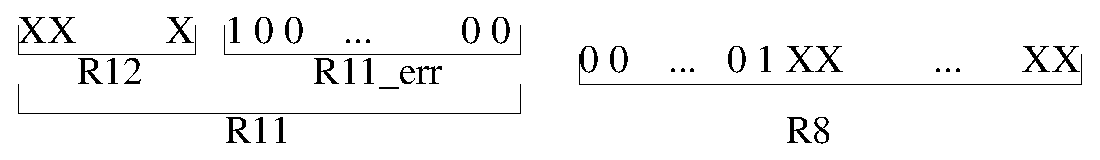
\includegraphics[width=0.5\textwidth]{rnd_to_nearest_pp.eps}
%   \end{center} 
%\end{figure}

%\begin{figure}[!htb]  
%  \begin{center}
%    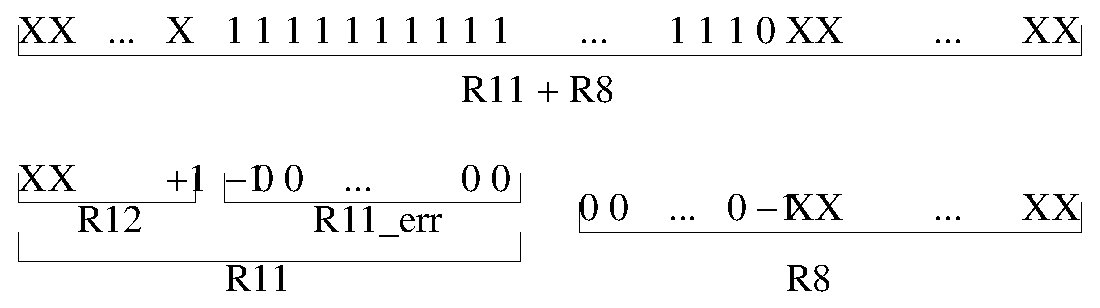
\includegraphics[width=0.5\textwidth]{rnd_to_nearest_mm.eps}
%  \end{center} 
%\end{figure}

\begin{figure}[ht] \begin{center}
\input{fig_exp/rnd_to_nearest.pstex_t}
\caption{Description of problem with rounding to nearest of a subnormal number.
  \label{chap4:fig:rnd_to_nearest}}
\end{center}\end{figure}


 
\subsection{Rounding toward $+ \infty$}
\begin{lstlisting}[caption={Test if rounding toward $+ \infty$ is possible}]
static const union{int i[2]; double d;}
#ifdef BIG_ENDIAN
 _two1000    = {0x7E700000, 0x00000000}, /*  1.07150860718626732095e301  */
 _twom1000   = {0x01700000, 0x00000000}, /*  9.33263618503218878990e-302 */
#else
 ...
#endif
#define two1000    _two1000.d
#define twom1000   _twom1000.d


int errd        = 71303168;                    /* 68 * 2^20 */  

int    exp_R11;
union {int i[2]; long long int l; double d;} R12;

/* Result = (R11 + R8) */

exp_R11 = (HI(R11) & 0x7ff00000) - errd;

if ((HI(R8) & 0x7ff00000) > exp_R11){      (*@ \label{exp:code:pinf:0} @*)
  /* We are able to round the result */
  if (k > -1020){                          
    if (k < 1020){                         
      HI(R11) += (k<<20);                  
    }else {
      /* We are close to + Inf */
      HI(R11) += ((k-1000)<<20);           
      R11 *= two1000;
    }
    if (HI(R8) > 0){                       (*@ \label{exp:code:pinf:1} @*)
      R12.d  = R11;
      R12.l += 1;
      R11    = R12.d;
    }
    return R11;
  }else {
    /* We are with subnormal number */
    HI(R11) += ((k+1000)<<20);          
    R12.d    = R11 * twom1000;              (*@ \label{exp:code:pinf:2} @*)

    HI(st2mem) = R12.i[HI] ;     
    LO(st2mem) = R12.i[LO]       

    R11 -= st2mem * two1000;                (*@ \label{exp:code:pinf:3} @*)
    if ((HI(R11) > 0)||((HI(R11) == 0)&&(HI(R8) > 0))) R12.l += 1;(*@ \label{exp:code:pinf:5} @*)

    return R12.d;
  }
}else {
  /* Difficult case */
  su_exp(x);
}
\end{lstlisting}


\begin{preuve}

The program used to check whether correct rounding toward $+ \infty$ is possible is similar to the one used with rounding to nearest.

\begin{longtable}[c]{@{line }p{0.08\textwidth}p{0.81\textwidth}}
% en cas de cesure c'est ce que l'on place 
% en debut de page
\endhead
% en fin de page
\endfoot 
% en fin de derniere page
\endlastfoot 
\ref{exp:code:pinf:0} & 
This test is valid even if the final result is a subnormal number.
\\

\ref{exp:code:pinf:1} &
We add $1 ulp$ to the result if $R8$ is positive. 
\\

\ref{exp:code:pinf:3} &
Like for rounding to nearest, the quantity $R11$ represent the rounding error that come from the operation $R11* twom1000$ in line \ref{exp:code:pinf:2}.
\\

\ref{exp:code:pinf:5} &
This test check whether the error from line \ref{exp:code:pinf:2} is strictly positive or if it is equal to zero and if $R8$ is strictly positive. If we are in one of these two cases, by definition of rounding toward $+ \infty$, we need to add $1 ulp$ to the result.
\end{longtable}
\end{preuve}


 
\subsection{Rounding toward $- \infty$}

\begin{lstlisting}[caption={Test if rounding toward $- \infty$ is possible},firstnumber = 144]
static const union{int i[2]; double d;}
#ifdef BIG_ENDIAN
 _two1000    = {0x7E700000, 0x00000000}, /*  1.07150860718626732095e301  */
 _twom1000   = {0x01700000, 0x00000000}, /*  9.33263618503218878990e-302 */
#else
 ...
#endif
#define two1000    _two1000.d
#define twom1000   _twom1000.d

int errd        = 71303168;                    /* 68 * 2^20 */  

int    exp_R11;
union {int i[2]; long long int l; double d} R12;
 
/* R�sult = (R11 + R8) */

exp_R11 = (HI(R11) & 0x7ff00000) - errd;

if ((HI(R8) & 0x7ff00000) > exp_R11){
  /* We are able to round the result */
  if (k > -1020){                          
    if (k < 1020){                         
      HI(R11) += (k<<20);                  
    }else {
      /* We are close to + Inf */
      HI(R11) += ((k-1000)<<20);           
      R11 *= two1000;
    }
    if (HI(R8) > 0){
      R12.d  = R11;
      R12.l += 1;
      R11    = R12.d;
    }
    return R11;
  }else {
    /* We are with subnormal number */
    HI(R11) += ((k+1000)<<20);             
    R12.d    = R11 * twom1000;             

    HI(st2mem) = R12.i[HI];                  
    LO(st2mem) = R12.i[LO];                  

    R11 -= st2mem * two1000;               
    if ((HI(R11) < 0)||((HI(R11) == 0)&&(HI(R8) < 0))) R12.l -= 1;

    return R12.d;
  }
}else {
  /* Difficult case */
  su_exp(x);
}
\end{lstlisting}



\begin{preuve}

The program used to check whether correct rounding toward $- \infty$ is possible is similar to the previous one and it work for similar reasons.
\end{preuve}


 
\subsection{Rounding toward $0$} 
The program used to check whether correct rounding toward $0$ is possible is identical to the one used for rounding to $- \infty$ because $\exp(x)$ is a positive function.

%%
%% 
%%
\section{Accurate phase}
\label{section:accurate_phase}
When the previous computation failed, it mean that the rounding of the result is difficult to get. We need to use more accurate methods :
\begin{itemize}
\item
 $sn\_exp$ with rounding to nearest,
\item
 $su\_exp$ with rounding toward $+\infty$,
\item
 $sd\_exp$ with rounding toward $-\infty$,
\end{itemize}

These methods are based on SCS library \cite{SCSweb}, with $30$ bits of precision per digits and $8$ digits per vector. The guarantee precision with this format is $211$ bits at least. Even if there is no proof for these operators yet, the proof for correct rounding of the exponential only request the following property  that are easy to check and/or satisfy :

\begin{propriete}(Addition)
Let $a \boxplus b$ represent the multiprecision operation performing an addition between $a$ and $b$ with at least $210$ bits of precision for the result. Like for double precision floating point number, the scs addition may leads to a cancellation. We have :
$$
a+ b = (a \boxplus b).(1+\epsilon_{-211})
$$
\end{propriete}

\begin{propriete}(Multiplication)
Let $a \boxtimes b$ represent the multiprecision operation performing a multiplication between $a$ and $b$ with at least $210$ bits of precision for the result. This operation do not produce a cancellation.
$$
a\times b = (a \boxtimes b).(1+\epsilon_{-211})
$$
\end{propriete}



\subsection{Overview of the algorithm}
Here is the algorithm used for the second part of the evaluation :
\begin{enumerate}
\item
{\bf No special case handeling} \\
For this part, we assume that test for special case handeling have been done.
\item
{\bf Range reduction} \\
We compute the reduced argument $r$ and the integer $k$ such that :
$$
r = \frac{x - k . \ln(2)}{512}
$$

with
$\frac{-\ln(2)}{1024} \leq r \leq \frac{-\ln(2)}{1024}$

such that
$$
\exp(x) = \exp(r)^{512} \times 2^{k}
$$


\item
{\bf Polynomial evaluation} \\
We compute the polynom $P(r)$ of degree 10 :
$$
\exp(r) = (1 + r + P(r)).(1+ \epsilon_{-164})
$$

\item
{\bf Powering the result} \\
$\exp(r)^{512} = \left(\left(\left(\left(\left(\left(\left(\left(\exp(r)^2\right)^2\right)^2\right)^2\right)^2\right)^2\right)^2\right)^2\right)^2$



\item
{\bf Reconstruction} \\
$$
\exp(x) = \exp(r)^{512}. 2^{k} . (1+\epsilon)
$$
avec $|\epsilon| \leq 2^{-163} $
\end{enumerate}

We have choosen this evaluation scheme, because the reconstruction step use the squaring multiprecision operator. This operator facilitate the error computation and is very economic : its cost is $0.7$ times the one of a true multiprecision multiplication.

We will notice that there exist an alternative to the squaring solution. We can tabulate values $2^{\frac{N}{512}}$ for $N=1,2,\ldots,511$ and use the formulae $\exp(x) = \exp(r) \times 2^{N} \times 2^{\frac{M}{512}}$ with $k=M+N/512$. However we prefer the squaring method that do not request the storage of SCS number and the associated quantity of memory.



\subsection{Function's call}
With Lef\`evre worst cases on table makers dilemma we get the following theorem :

\begin{theorem}(Correct rounding for the exponential)
Let $y$ be the exact value of the exponential of a floating-point number in double precision $x$. Let $y^*$ be an approximation of $y$ such that the distance between $y$ and $y^*$ be bounded by $\epsilon$. Then if $\epsilon \leq 2^{-157}$, for each of the four rounding mode, rounding $y^*$ is equivalent to rounding $y$;
\end{theorem}

To round the multiprecision result in SCS format depending on the rounding mode, we use the following procedure (\texttt{scs\_get\_d}, \texttt{scs\_get\_d\_pinf}, \texttt{scs\_get\_d\_minf}). 

\subsubsection{Rounding to nearest}

\begin{lstlisting}[caption={Compute the rounding to nearest of the exponential in multiprecision},firstnumber=1]
double sn_exp(double x){ 
  scs_t res_scs;
  scs_db_number res;

  exp_SC(res_scs, x);
  scs_get_d(&res.d, res_scs);  res.d = x;

  return res.d;
}
\end{lstlisting}



\subsubsection{Rounding toward $+ \infty$}

\begin{lstlisting}[caption={Compute the rounding toward $+ \infty$ of the exponential in multiprecision},firstnumber=1]
double su_exp(double x){ 
  scs_t res_scs;
  scs_db_number res;
  
  exp_SC(res_scs, x);
  scs_get_d_pinf(&res.d, res_scs);
  return res.d;
}
\end{lstlisting}



\subsubsection{Rounding toward $- \infty$}

\begin{lstlisting}[caption={Compute the rounding toward $- \infty$ of the exponential in multiprecision},firstnumber=1]
double sd_exp(double x){ 
  scs_t res_scs;
  scs_db_number res;
  
  exp_SC(res_scs, x);
  scs_get_d_minf(&res.d, res_scs);
  return res.d;
}
\end{lstlisting}



\subsection{Software}
The function $exp\_SC$ approximate the exponential of $x$ with $163$ bits of precision and put the result in $res\_scs$.

\begin{lstlisting}[caption={Compute the exponential in multiprecision},firstnumber=1]
void exp_SC(scs_ptr res_scs, double x){
  scs_t sc1, red;
  scs_db_number db;
  int i, k;


  /* db.d = x/512  (= 2^9)  */
  
  db.d = x;                                    (*@ \label{exp:mp:0} @*)
  db.i[HI] -= (9 << 20);                (*@ \label{exp:mp:1} @*) 
  scs_set_d(sc1, db.d);                        (*@ \label{exp:mp:2} @*)
  
  
  DOUBLE2INT(k, (db.d * iln2_o512.d));         (*@ \label{exp:mp:3} @*) 
 
  /* 1) Range reduction */
  
  scs_set(red,     sc_ln2_o512_ptr_1);;        (*@ \label{exp:mp:4} @*)             
  scs_set(red_low, sc_ln2_o512_ptr_2);         (*@ \label{exp:mp:4b} @*)      
  if (k>0){
    scs_mul_ui(red,      (unsigned int) k);
    scs_mul_ui(red_low,  (unsigned int) k);
  }else {
    scs_mul_ui(red,      (unsigned int)(-k));
    scs_mul_ui(red_low,  (unsigned int)(-k));
    red->sign *= -1;
    red_low->sign *=-1;
  }                                            (*@ \label{exp:mp:5} @*)

  scs_sub(red, sc1, red);                      (*@ \label{exp:mp:6} @*)
  scs_sub(red, red, red_low);                  (*@ \label{exp:mp:6b} @*)

  
  /* 2) Polynomial evaluation */               (*@ \label{exp:mp:7} @*)
   
  scs_mul(res_scs, constant_poly_ptr[0], red);
  for(i=1; i< 10; i++){                       
    scs_add(res_scs, constant_poly_ptr[i], res_scs);
    scs_mul(res_scs, red, res_scs);            
  }
  
  scs_add(res_scs, SCS_ONE, res_scs);          
  scs_mul(res_scs, red, res_scs);
  scs_add(res_scs, SCS_ONE, res_scs);          (*@ \label{exp:mp:8} @*)  

  /* 3) Powering the result exp(r)^512  */
  
  for(i=0; i<9; i++){                          (*@ \label{exp:mp:9} @*)
    scs_square(res_scs, res_scs);
  }

  /* 4) Multiplication by 2^k */
  
  res_scs->index += (int)(k/30);               (*@ \label{exp:mp:10} @*)
  if ((k%30) > 0) 
    scs_mul_ui(res_scs, (unsigned int) (1<<((k%30))));
  else if ((k%30) < 0){
    res_scs->index --;
    scs_mul_ui(res_scs, (unsigned int) (1<<((30+(k%30)))));
  }                                            (*@ \label{exp:mp:11} @*)

}

\end{lstlisting}



\begin{preuve}
\begin{longtable}[c]{@{line }p{0.08\textwidth}p{0.81\textwidth}}
% en cas de cesure c'est ce que l'on place 
% en debut de page
\endhead
% en fin de page
\endfoot 
% en fin de derniere page
\endlastfoot 
\ref{exp:mp:0}& $db.d = x$
\\
\ref{exp:mp:1}& 
This operation divide  $db.d$ by $512=2^9$ and is valid under the condition that $db.d$, and consequently $x$, do not represent a special values (subnormal, infinity, NaN). Condition that is satisfied because special case have been treated during the quick phase.

\\
\ref{exp:mp:2}& 
$sc1$ is a $211$ bits multiprecision number such that :
\begin{prop}
  \label{chap3:exp:mp:prop0}
 $sc1=db.d = \frac{x}{512}$ exactly
\end{prop}
\\
\ref{exp:mp:3}& $iln2\_o512.d$ is a double precision floating-point number such that :
$iln2\_o512.d = \frac{512}{\ln{2}}(1 + \epsilon_{-54})$. This line put in $k$ the closest integer of $db.d \otimes \frac{512}{\ln{2}}$. We use the property of $DOUBLE2INT$ which convert a floating-point number in an integer with rounding to nearest.

Moreover $k$ satisfy the following property :
\begin{prop}
  \label{chap3:exp:mp:prop1}
  $$
\lfloor \frac{x}{\ln 2} \rfloor  \leq k \leq   \lceil \frac{x}{\ln 2} \rceil
   ~~~ \mbox{et} ~~~   -1075 \leq |k| \leq 1025
$$
\end{prop}
And $k$ is a $11$ bits integer.
\\
\ref{exp:mp:4}, \ref{exp:mp:4b}&
By construction we have :
$$red + red\_low = \frac{\ln 2}{512}(1 + \epsilon_{-450})$$
and $red$ is construct in order to make the multiplication of $red$ by $k$ exact if $|k| \leq 2^{11}$.

\\
\ref{exp:mp:5}&
At the end of the test on $k$ we have : 
$red + red\_low = k \otimes \frac{\ln 2}{512}(1 + \epsilon_{-450})$

with $|k| < 2^{11}$, then :
\begin{prop}
  \label{chap3:exp:mp:prop2}
$$red  + red\_low = k \times \frac{\ln 2}{512}(1 + \epsilon_{-411})$$
\end{prop}
\\
\ref{exp:mp:6},\ref{exp:mp:6b}&
By the properties \pref{chap3:exp:mp:prop0} and \pref{chap3:exp:mp:prop2} we have :
\begin{prop}
  \label{chap3:exp:mp:prop3}
$red = \frac{x}{512} \ominus \left( k \times \frac{\ln 2}{512} \right) (1 + \epsilon_{-411})$
\end{prop}

In addition we have seen in the quick phase that at most $58$ bits could be cancelled, during this subtraction.
\begin{prop}
  \label{chap3:exp:mp:prop4}
$|red| \leq \frac{\ln 2}{1024} \leq 2^{-10}$,

$red = \frac{x}{512} - k \times \frac{\ln 2}{512}  + \epsilon_{-211} $
\end{prop}
\\
\ref{exp:mp:7}-\ref{exp:mp:8}&
We now perform the polynomial evaluation where the coefficient have the following properties.
\begin{prop}
  \label{chap3:exp:mp:prop5}
$|constant\_poly\_ptr[0]=c_0| \leq 2^{-25}$, $|constant\_poly\_ptr[1]=c_1| \leq 2^{-21}$,
$|constant\_poly\_ptr[2]=c_2| \leq 2^{-18}$, $|constant\_poly\_ptr[3]=c_3| \leq 2^{-15}$,
$|constant\_poly\_ptr[4]=c_4| \leq 2^{-12}$, $|constant\_poly\_ptr[5]=c_5| \leq 2^{-9}$,
$|constant\_poly\_ptr[6]=c_6| \leq 2^{-6}$,  $|constant\_poly\_ptr[7]=c_7| \leq 2^{-4}$,
$|constant\_poly\_ptr[8]=c_8| \leq 2^{-2}$,  $|constant\_poly\_ptr[9]=c_9| \leq 2^{-1}$
\end{prop}


We have :
\begin{itemize}
\item $P_0=c_1 \boxplus (red \boxtimes c_0)$   thus $|P_0| \leq 2^{-20}$ et $P_0 = c_1 + (red \times c_0 ) + \epsilon_{-231}$
\item $P_1=c_2 \boxplus (red \boxtimes P_0)$   thus $|P_1| \leq 2^{-17}$ et $P_1 = c_2 + (red \times P_0 ) + \epsilon_{-228}$
\item $P_2=c_3 \boxplus (red \boxtimes P_1)$   thus $|P_2| \leq 2^{-14}$ et $P_2 = c_3 + (red \times P_1 ) + \epsilon_{-225}$
\item $P_3=c_4 \boxplus (red \boxtimes P_2)$   thus $|P_3| \leq 2^{-11}$ et $P_3 = c_4 + (red \times P_2 ) + \epsilon_{-222}$
\item $P_4=c_5 \boxplus (red \boxtimes P_3)$   thus $|P_4| \leq 2^{-8}$ et $P_4 = c_5 + (red \times P_3 ) + \epsilon_{-219}$
\item $P_5=c_6 \boxplus (red \boxtimes P_4)$   thus $|P_5| \leq 2^{-5}$ et $P_5 = c_6 + (red \times P_4 ) + \epsilon_{-216}$
\item $P_6=c_7 \boxplus (red \boxtimes P_5)$   thus $|P_6| \leq 2^{-3}$ et $P_6 = c_7 + (red \times P_5 ) + \epsilon_{-214}$
\item $P_7=c_8 \boxplus (red \boxtimes P_6)$   thus $|P_7| \leq 2^{-1}$ et $P_7 = c_8 + (red \times P_6 ) + \epsilon_{-212}$
\item $P_8=c_9 \boxplus (red \boxtimes P_7)$   thus $|P_8| \leq 1 + 2^{-10} $ et $P_8 = c_9 + (red \times P_7 ) + \epsilon_{-211}$
\item $P_9=1   \boxplus (red \boxtimes P_8)$   thus $|P_9| \leq 1 + 2^{-9}$ et $P_9 = 1   + (red \times P_8 ) + \epsilon_{-210}$
\item $P_{10}=1   \boxplus (red \boxtimes P_9)$ thus $|P_{10}| \leq 1 + 2^{-8}$ et $P_{10} = 1   + (red \times P_9) + \epsilon_{-210}$
\end{itemize}

Therefore :
$$
res\_scs = P_{10} + \epsilon_{-208}
$$ 

We build the polynom such that  
$$\exp(r) = (1 + r + c_9. r^2 + \cdots + c_0 . r^{11}).(1 + \epsilon_{-164})$$
Therefore

$|res\_scs| \leq 1 + 2^{-8}$
with

$\exp(red) = (res\_scs  + \epsilon_{-208}).(1 + \epsilon_{-164})$
\\

\ref{exp:mp:9}&
We perform a squaring of the result $9$ times, that correspond to powering the result to the power $512$. 
At each iteration we perform a rounding error equal to $\epsilon_{-211}$.

Finally :

$|res\_scs| \leq  2^{3}$
and

$\exp(x) = 2^k. (res\_scs  + \epsilon_{-199}).(1 + \epsilon_{-164})$
\\
\ref{exp:mp:10}-\ref{exp:mp:11}&
With these lines we perform the multiplication of $res\_scs$ by $2^k$. This multiplication is done by a shift on the index of $k/30$, where $30$ correspond to the number of bits used within a multiprecision number. This shift is exact. Then a multiplication of $res\_scs$ by $2$ to the power the rest of the euclidian division of $k$ by $30$ is done. At the end of these instructions we have :
$$\exp(x) = (res\_scs).(1 + \epsilon_{-163})$$

\\

\end{longtable}
\end{preuve}




%%%%%%%%%%%%%%%%%%%%%%%%%%%%%%%%%%%%%%%%%%%%%%%%%%%%%%%%%%%%%
\section{Analysis of the exponential}
\label{section:exp_results}

\subsection{Test conditions}

Table \ref{tbl:systems} lists the combinations of processor, OS and
default \texttt{libm} used for our tests.
\begin{table}[!htb]
\begin{center}
\renewcommand{\arraystretch}{1.2}
\begin{tabular}{|c||c|c|c|}
\hline
Processor        & OS & compiler & default \texttt{libm} \\
\hline
\hline
Pentium III      & Debian GNU/Linux & gcc-2.95          & \texttt{glibc}, derived from \texttt{fdlibm} \\ 
\hline
UltraSPARC IIi   & SunOS 5.8        & gcc-2.95          & \texttt{fdlibm} \\
\hline
Xeon (Pentium 4) & Debian GNU/Linux & gcc-2.95          & \texttt{glibc}, derived from \texttt{fdlibm}\\
\hline
PowerPC G4       & MacOS 10.2       & gcc-2.95          & Apple specific \\
\hline
Itanium          & Debian GNU/Linux & gcc-2.95, gcc-3.2 & Intel optimized \\
\hline
\end{tabular}
\end{center}
\caption{The systems tested
  \label{tbl:systems}}
\end{table}

The following presents tests
performed under such conditions as to suppress most of the impact of
the memory hierarchy: A small loops performs 10 identical calls to
the function, and the minimum timing is reported, ensuring that both
code and data have been loaded in the cache, and that interruptions by
the operating system do not alter the timings.

These timings are taken on random values between $-745$ and $+744$,
which is the practical range for the exponential. We also report the
timing for the worse case for the correct rounding in rounding to
nearest mode of the exponential, which is
$x=7.5417527749959590085206221e-10$.

Our libray was tuned to take into account the adequation of the evaluation scheme to the memory hierarchies of current processors (our program for the exponential evaluation uses $2.8$Kbytes of table for the four rounding modes, whereas the one from \emph{fdlibm} use $13$Kbytes). However we do not have tested the impact over performance of this concern and is part of our futur works. 

\subsection{Results}

Tables \ref{tbl:exp_abstime} gives a summary of the timings of the
various libraries. The \accurate\ phase is called about 2 times out of 100000.


\begin{table}[!htb]
\begin{center}
\renewcommand{\arraystretch}{1.2}
\begin{tabular}{|l|r|r|r|}
\hline
 \multicolumn{4}{|c|}{Pentium 4 Xeon / Linux Debian sarge / gcc 3.3}   \\ 
 \hline
 \hline
 \texttt{libm}           & 236          & 5528          &        365 \\ 
 \hline
  \texttt{mpfr}          & 14636        & 204736        &      23299 \\ 
 \hline
  \texttt{libultim}      & 44           & 3105632       &        210 \\ 
 \hline
 \texttt{crlibm}         & 316          & 41484         &        432 \\ 
 \hline
 \hline
  \multicolumn{4}{|c|}{PowerPC G4 / MacOS X / gcc2.95}   \\
 \hline
                         & min time      & max time      & avg time \\
 \hline
 \texttt{libm}           & 7            & 14            &         12 \\
 \hline
  \texttt{mpfr}          & 972          & 2819          &       1367 \\
 \hline
  \texttt{libultim}      & 8            & 169390        &         12 \\
 \hline
 \texttt{crlibm}         & 4            & 916           &         15 \\
 \hline
\end{tabular}
\end{center}
\caption{Absolute timings for the exponential (arbitrary units)
  \label{tbl:exp_abstime}}
\end{table}





\subsection{Analysis}

\subsubsection*{Processor-specific libraries}
Documentation\cite{HarKubStoTan99} from Intel labs claim to provide an
exponential in only $48$ cycles. This performance is possible through
the wide use of non portable tricks such as inverse approximation,
fused multiply and add and double extended precision.  However, our
tests show that the environmental cost (mainly the cost of a function
call) is about $80$ clock cycles! Our tests have also shown that there
exists a slower path that takes up to $2767$ clock cycles, which is $14$ times slower. This path
seems to be taken very often since the average cost is $1.5$ times
more expensive than the smallest  execution time.

The same conclusion can be done for the mathematical library used on
Ultra-SPARC IIi system, where there exists a path $13$ times slower
than a normal execution.

These two observations show that our two-step procedure, with a much
slower second step, could be viable in the commercial world.

The mathematical library used on the PowerPC G4 with gcc is the one
from Apple. This library do not provide correct rounding and is $1.1$
slower than the version provided with \emph{crlibm}. It is, however,
the most accurate of the tested libraries.


\subsubsection*{The cost of correct rounding}

The \emph{libutlim} library provides correct rounding for an average
cost between $0.9$ (on a Pentium III) and $1.8$ (on an Itanium) times
the cost of the standard library. Our exponential give a result for an
average cost between $0.91$ (on Power-PC) and $2.66$ (on Ultra-SPARC
IIi) times the cost of the standard library, which is reasonable. On
the other hand, MPFR provide correct rounding for an average cost
between $13.5$ (on Power-PC) and $153$ (on Itanium) compared to the
\emph{libm}. 

The main advantage of \emph{crlibm} over \emph{libutlim} is the upper
bound on the execution time. On our tests, this bound for
\emph{crlibm} is $147$ times the average \emph{libm} cost, whereas for
\emph{libtultim} this bound goes up to $14499$ times the average
\emph{libm} cost. Our two steps strategy fully benefits from knowing
bounds on correct rounding worst cases.

We notice that our second step is in average $3$ times faster than the
multiprecision library MPFR. It shows that our multiprecision
operators from \emph{scslib}, hand tuned for $200$ bits of precision
perfectly fulfill the performance requirement of the second step.


\subsubsection*{Relations between the two steps of \emph{crlibm}}

Our second phase is $30$ times slower than the first step and is
called only once over $2^{13}$. The cost of the second step over the
average cost is :

$$
\frac{1 \times (2^{13}-1) + 30 \times 1}{2^{13}} = 1.003540039
$$
which corresponds to a $0.35\%$ overhead. This small overhead in
average  means that a possible performance improvement
is to reduce the precision of the first step, and by the same way the
number of instructions, to increase to number of time that the second
step is called. It will also make the proof simpler.


%%%%%%%%%%%%%%%%%%%%%%%%%%%%%%%%%%%%%%%%%%%%%%%%%%%%%%%%%%%%%
\section{Conclusion and perspectives}


 It is obvious from our performance measurements that our first step is
too accurate and too slow for a balanced average time. We will take
this experience into consideration when writing first steps for other
functions. The IBM library seems to get a better balance although its
second and later steps are much slower. Its code, unfortunately, is
little documented and difficult to prove.

Writing the proofs is a very time-consuming task, which could be
partially automated for one step which is common to most function: The
accumulation of error terms in order to compute the final error.



